%% abtex2-modelo-trabalho-academico.tex, v-1.9.6 laurocesar
%% Copyright 2012-2016 by abnTeX2 group at http://www.abntex.net.br/ 
%%
%% This work may be distributed and/or modified under the
%% conditions of the LaTeX Project Public License, either version 1.3
%% of this license or (at your option) any later version.
%% The latest version of this license is in
%%   http://www.latex-project.org/lppl.txt
%% and version 1.3 or later is part of all distributions of LaTeX
%% version 2005/12/01 or later.
%%
%% This work has the L PPL maintenance status `maintained'.
%% 
%% The Current Maintainer of this work is the abnTeX2 team, led
%% by Lauro César Araujo. Further information are available on 
%% http://www.abntex.net.br/
%%
%% This work consists of the files abntex2-modelo-trabalho-academico.tex,
%% abntex2-modelo-include-comandos and abntex2-modelo-references.bib
% ------------------------------------------------------------------------ 
% ------------------------------------------------------------------------
% abnTeX2: Modelo de Trabalho Academico (tese de doutorado, dissertacao de
% mestrado e trabalhos monograficos em geral) em conformidade com  
% ABNT NBR 14724:2011: Informacao e documentacao - Trabalhos academicos -
% Apresentacao
% ------------------------------------------------------------------------
% ------------------------------------------------------------------------
% Personalização para o modelo Udesc 2020 7. ed. revisada e modificada
% MANUAL_2020_09_07_1599489825065_12510.pdf
% Autor: Felipe Joel Zimann (felipezimann@hotmail.com)
% Data: 02/12/2020 v1.0
% Data: 13/02/2021 v1.0.1 alterado tamanho numeração da página para 10pt
% ------------------------------------------------------------------------
% ------------------------------------------------------------------------
  
\documentclass[
	12pt,					% tamanho da fonte
	openright,				% capítulos começam em pág ímpar (insere página vazia caso preciso)
	oneside,				% para impressão em recto e verso (twoside). Oposto a (oneside)
	a4paper,				% tamanho do papel. 
	chapter=TITLE,			% títulos de capítulos convertidos em letras maiúsculas
	section=TITLE,			% títulos de seções convertidos em letras maiúsculas
	sumario=abnt-6027-2012,
	english,				% idioma adicional para hifenização
	brazil,					% o último idioma é o principal do documento
	fleqn,					% equações alinhadas a esquerda (UDESC/CCT)+
	]{abntex2}

% ----------------------------------------------------------
% Pacotes básicos 
% ----------------------------------------------------------
\usepackage{amsmath}							% Pacote matemático
\usepackage{amssymb}							% Pacote matemático
\usepackage{amsfonts}							% Pacote matemático
%\usepackage{lmodern}							% Usa a fonte Latin Modern		
\usepackage{mathptmx} 							% Usa a fonte Times New Roman	 (UDESC/CCT)
\usepackage[T1]{fontenc}						% Selecao de codigos de fonte.
\usepackage[utf8]{inputenc}						% Codificacao do documento (conversão automática dos acentos)
\usepackage{lastpage}							% Usado pela Ficha catalográfica
\usepackage{indentfirst}						% Indenta o primeiro parágrafo de cada seção.
\usepackage[dvipsnames,table]{xcolor}			% Controle das cores
\usepackage{graphicx}							% Inclusão de gráficos
\usepackage{microtype} 							% para melhorias de justificação
\usepackage{lipsum}								% para geração de dummy text
\usepackage[brazilian,hyperpageref]{backref}	% Paginas com as citações na bibl
\usepackage[alf,abnt-emphasize=bf,abnt-full-initials=yes]{abntex2cite}					% Citações padrão ABNT
%\usepackage[num]{abntex2cite}					% Citações padrão ABNT numérica
\usepackage{adjustbox}							% Pacote de ajuste de boxes
\usepackage{subcaption}							% Inclusão de Subfiguras e sublegendas		
\usepackage{enumitem}							% Personalização de listas
\usepackage{siunitx}							% Grandezas e unidades
\usepackage[section]{placeins}					% Manter as figuras delimitadas na respectiva seção com a opção [section]
\usepackage{multirow}							% Multi colunas nas tabelas
\usepackage{array,tabularx} 					% Pacotes de tabelas
\usepackage{booktabs}							% Pacote de tabela profissonal
\usepackage{rotating}							% Rotacionar figuras e tabelas
\usepackage{xfrac}								% Fazer frações n/d em linha
\usepackage{bm}									% Negrito em modo matemático
\usepackage{xstring}							% Manipulação de strings
\usepackage{pgfplots}							% Pacote de Gráficos
\usepackage{tikz}								% Pacote de Figuras
\usepackage[american, cuteinductors,smartlabels, fulldiode, siunitx, americanvoltages, oldvoltagedirection, smartlabels]{circuitikz}						% Pacote de circuitos elétricos
\usepackage{chemformula}						% Pacote para fórmulas químicas
\usepackage{chngcntr}							% Pacte usado para deixar numeração de equações sequencial (UDESC/CCT)
\counterwithout{equation}{chapter}
% fonte: https://latex.org/forum/viewtopic.php?t=15392

% Comando para deixar numeração das equações contínua (1), (2), (3)... ao invés de organizar por capítulos (1.1)(1.2)... (2.1)(2.2)
%\renewcommand{\theequation}{\arabic{equation}}

%\numberwithin{equation}{section}


% Cabecalho cabeçalho somente com numeração de página 10pt
\makepagestyle{PagNumReduzida}
\makeevenhead{PagNumReduzida}{\ABNTEXfontereduzida\thepage}{}{}
\makeoddhead{PagNumReduzida}{}{}{\ABNTEXfontereduzida\thepage}
%fonte: https://github.com/abntex/abntex2/wiki/HowToCustomizarCabecalhoRodape
%fonte: Manual memoir seção 7.3 pg. 111 pdf http://linorg.usp.br/CTAN/macros/latex/contrib/memoir/memman.pdf 

% Personalização das opções das listas
\setlist[itemize]{leftmargin=\parindent}

% Citação online --- MODIFICAR ---
\newcommand{\citeshort}[1]{\citeauthoronline{#1}~(\citeyear{#1})}

\newcommand{\me}[1]{Elaborado pelo autor (#1).}

% Configuração do pgfplots
\pgfplotsset{compat=newest} %compat=1.14
\pgfplotsset{plot coordinates/math parser=false} 
\newlength\figureheight 
\newlength\figurewidth 

% Libraries do TiKz
\usetikzlibrary{quotes,angles,arrows}
\usetikzlibrary{through,calc,math}
\usetikzlibrary{graphs,backgrounds,fit}
\usetikzlibrary{shapes,positioning,patterns,shadows}
\usetikzlibrary{decorations.pathreplacing}
\usetikzlibrary{shapes.geometric}
\usetikzlibrary{arrows.meta}
\usetikzlibrary{external}

%\tikzexternalize[]
%\tikzexternalenable
%\tikzexternalize
%\tikzexternaldisable
%\tikzset{external/force remake}
%\tikzexternalize[shell escape=-enable-write18]

% Configurações do CircuiTiKz
\ctikzset{bipoles/thickness=1}
%\ctikzset{bipoles/length=1.2cm}
\ctikzset{monopoles/ground/width/.initial=.2}
\ctikzset{bipoles/resistor/height=0.25}
\ctikzset{bipoles/resistor/width=0.6}
\ctikzset{bipoles/capacitor/height=0.5}
\ctikzset{bipoles/capacitor/width=0.15}
\ctikzset{bipoles/generic/height=0.25}
\ctikzset{bipoles/generic/width=0.6}
%\ctikzset{bipoles/capacitor polar/length=0.5}
%\ctikzset{bipoles/diode/height=.375}
%\ctikzset{bipoles/diode/width=.3}
%\ctikzset{tripoles/thyristor/height=.8}
%\ctikzset{tripoles/thyristor/width=1}
\ctikzset{bipoles/vsourcesin/height=.5}
\ctikzset{bipoles/vsourcesin/width=.5}
\ctikzset{bipoles/cvsourceam/height=.6}
\ctikzset{bipoles/cvsourceam/width=.6}
%\ctikzset{tripoles/european controlled voltage source/width=.4}

\tikzstyle{every node}=[font=\footnotesize]
\tikzstyle{every path}=[line width=0.25pt,line cap=round,line join=round]
%\tikzstyle{every path}=[line cap=round,line join=round]


% Definição de cores MATLAB
\definecolor{matlab_blue}{rgb}	{         0,    0.4470,    0.7410}
\definecolor{matlab_orange}{rgb}{    0.8500,    0.3250,    0.0980}
\definecolor{matlab_yellow}{rgb}{    0.9290,    0.6940,    0.1250}
\definecolor{matlab_violet}{rgb}{    0.4940,    0.1840,    0.5560}
\definecolor{matlab_green}{rgb}	{	 0.4660,    0.6740,    0.1880}
\definecolor{matlab_lblue}{rgb}	{    0.3010,    0.7450,    0.9330}
\definecolor{matlab_red}{rgb}	{    0.6350,    0.0780,    0.1840}

% Personalização das legendas
\usepackage[format = plain, %hang
			justification = centering,
			labelsep = endash,
			singlelinecheck = false,
			skip = 6pt,
			listformat = simple]{caption}	

% Personalização das unidades
\sisetup{output-decimal-marker = {,}}
\sisetup{exponent-product = \cdot, output-product = \cdot}
\sisetup{tight-spacing=true}
\sisetup{group-digits = false}

% Personalizações de tipo de colunas de tabelas
\newcolumntype{L}[1]{>{\raggedright\let\newline\\\arraybackslash\hspace{0pt}}m{#1}}
\newcolumntype{C}[1]{>{\centering\let\newline\\\arraybackslash\hspace{0pt}}m{#1}}
\newcolumntype{R}[1]{>{\raggedleft\let\newline\\\arraybackslash\hspace{0pt}}m{#1}}

% Personalizações de cores da UDESC
\definecolor{CapaAmareloUDESC}{RGB}{243,186,83}		% Especializacao
\definecolor{CapaVerdeUDESC}{RGB}{0,112,52}			% Mestrado
\definecolor{CapaVermelhoUDESC}{RGB}{171,35,21}		% Doutorado
\definecolor{CapaAzulUDESC}{RGB}{38,54,118} 		% Pós-Doutorado

% CONFIGURAÇÕES DE PACOTES
% Configurações do pacote backref
% Usado sem a opção hyperpageref de backref
\renewcommand{\backrefpagesname}{Citado na(s) página(s):~}
% Texto padrão antes do número das páginas
\renewcommand{\backref}{}
% Define os textos da citação
\renewcommand*{\backrefalt}[4]{
	\ifcase #1 %
	Nenhuma citação no texto.%
	\or
	Citado na página #2.%
	\else
	Citado #1 vezes nas páginas #2.%
	\fi}%

% alterando o aspecto da cor azul
%\definecolor{blue}{RGB}{41,5,195}

% informações do PDF
\makeatletter
\hypersetup{
	%pagebackref=true,
	pdftitle={\@title}, 
	pdfauthor={\@author},
	pdfsubject={\imprimirpreambulo},
	pdfcreator={LaTeX with abnTeX2},
	pdfkeywords={abnt}{latex}{abntex}{abntex2}{trabalho academico}, 
	colorlinks=true,       		% false: boxed links; true: colored links
	linkcolor=black,          	% color of internal links
	citecolor=black,        	% color of links to bibliography
	filecolor=black,      		% color of file links
	urlcolor=black,
	bookmarksdepth=4
}
\makeatother


\makeatletter
\newcommand{\includetikz}[1]{%
	\tikzsetnextfilename{#1}%
	\input{#1.tex}%
}
\makeatother

% ---
% Possibilita criação de Quadros e Lista de quadros.
% Ver https://github.com/abntex/abntex2/issues/176
%
\newcommand{\quadroname}{Quadro}
\newcommand{\listofquadrosname}{Lista de quadros}

\newfloat[chapter]{quadro}{loq}{\quadroname}
\newlistof{listofquadros}{loq}{\listofquadrosname}
\newlistentry{quadro}{loq}{0}

% configurações para atender às regras da ABNT
\setfloatadjustment{quadro}{\centering}
\counterwithout{quadro}{chapter}
\renewcommand{\cftquadroname}{\quadroname\space} 
\renewcommand*{\cftquadroaftersnum}{\hfill--\hfill}

\setfloatlocations{quadro}{hbtp} % Ver https://github.com/abntex/abntex2/issues/176
% ---


% Espaçamento depois do título
\setlength{\afterchapskip}{0.7\baselineskip}
% O tamanho do parágrafo é dado por:
\setlength{\parindent}{1.25cm}
% Controle do espaçamento entre um parágrafo e outro:
\setlength{\parskip}{0.0cm}  % tente também \onelineskip
%\SingleSpacing % Espaçamento simples 
\OnehalfSpacing % Espaçamento 1,5 (UDESC/CCT)
%\DoubleSpacing	% Espaçamento duplo

% ---
% Margens - NBR 14724/2011 - 5.1 Formato
% ---
\setlrmarginsandblock{3cm}{2cm}{*}
\setulmarginsandblock{3cm}{2cm}{*}
\checkandfixthelayout[fixed]
% ---


% To use externalize consider
%https://tex.stackexchange.com/questions/182783/tikzexternalize-not-compatible-with-miktex-2-9-abntex2-package
%Lauro Cesar digged into the problem until he came with a solution for me to test. And it Works!
%
%According to this link:
%
%The package calc changed the commands \setcounter and friends to be fragile. So you have to make them robust. The example below uses etoolbox with \robustify:
%
\usepackage{etoolbox}
\robustify\setcounter
\robustify\addtocounter
\robustify\setlength
\robustify\addtolength


%% How to silence memoir class warning against the use of caption package?
%% https://tex.stackexchange.com/questions/391993/how-to-silence-memoir-class-warning-against-the-use-of-caption-package
%\usepackage{silence}
%\WarningFilter*{memoir}{You are using the caption package with the memoir class}
%\WarningFilter*{Class memoir Warning}{You are using the caption package with the memoir class}

% --------------------------------------------------------
% INICIO DAS CUSTOMIZACOES PARA A UDESC
% --------------------------------------------------------

% --------------------------------------------------------
% Fontes padroes de part, chapter, section, subsection e subsubsection
% --------------------------------------------------------
% --- Chapter ---
\renewcommand{\ABNTEXchapterfont}{\fontseries{b}} %\bfseries
\renewcommand{\ABNTEXchapterfontsize}{\normalsize}
% --- Part ---
\renewcommand{\ABNTEXpartfont}{\ABNTEXchapterfont}
\renewcommand{\ABNTEXpartfontsize}{\LARGE}
% --- Section ---
\renewcommand{\ABNTEXsectionfont}{\normalfont}
\renewcommand{\ABNTEXsectionfontsize}{\normalsize}
% --- SubSection ---
\renewcommand{\ABNTEXsubsectionfont}{\fontseries{b}} %\bfseries
\renewcommand{\ABNTEXsubsectionfontsize}{\normalsize}
% --- SubSubSection ---
\renewcommand{\ABNTEXsubsubsectionfont}{\itshape}
\renewcommand{\ABNTEXsubsubsectionfontsize}{\normalsize}

\renewcommand{\ABNTEXsubsubsubsectionfont}{\normalfont}
\renewcommand{\ABNTEXsubsubsubsectionfontsize}{\normalsize}
% ---

% --------------------------------------------------------
% Fontes das entradas do sumario
% --------------------------------------------------------

\renewcommand{\cftpartfont}{\ABNTEXpartfont\selectfont}
\renewcommand{\cftpartpagefont}{\normalsize\selectfont}

\renewcommand{\cftchapterfont}{\ABNTEXchapterfont\selectfont}
\renewcommand{\cftchapterpagefont}{\normalsize\selectfont}

\renewcommand{\cftsectionfont}{\ABNTEXsectionfont\selectfont}
\renewcommand{\cftsectionpagefont}{\normalsize\selectfont}

\renewcommand{\cftsubsectionfont}{\ABNTEXsubsectionfont\selectfont}
\renewcommand{\cftsubsectionpagefont}{\normalsize\selectfont}

\renewcommand{\cftsubsubsectionfont}{\normalfont\itshape\selectfont}
\renewcommand{\cftsubsubsectionpagefont}{\normalsize\selectfont}

\renewcommand{\cftparagraphfont}{\normalfont\selectfont}
\renewcommand{\cftparagraphpagefont}{\normalsize\selectfont}

% --------------------------------------------------------
% Usando os pacotes hyperref, uppercase... 
% Para deixar a section do toc uppercase precisa de:
% --------------------------------------------------------
\usepackage{textcase}

\makeatletter

\let\oldcontentsline\contentsline
\def\contentsline#1#2{%
	\expandafter\ifx\csname l@#1\endcsname\l@section
	\expandafter\@firstoftwo
	\else
	\expandafter\@secondoftwo
	\fi
	{%
		\oldcontentsline{#1}{\MakeTextUppercase{#2}}%
	}{%
		\oldcontentsline{#1}{#2}%
	}%
}
\makeatother

% --------------------------------------------------------
% Renomenando as entradas de APÊNDICES E ANEXOS
% --------------------------------------------------------

\renewcommand{\apendicesname}{AP\^ENDICES}
\renewcommand{\anexosname}{ANEXOS}


% Manipulação de Strings
%\RequirePackage{xstring}

% Comando para inverter sobrenome e nome
\newcommand{\invertname}[1]{%
	\StrBehind{#1}{{}}, \StrBefore{#1}{{}}%
}%


% --------------------------------------------------------
% Alterando os estilos de Caption e Fonte
% --------------------------------------------------------
\makeatletter
% Define o comando \fonte que respeita as configurações de caption do memoir ou do caption
\renewcommand{\fonte}[2][\fontename]{%
	\M@gettitle{#2}%
	\memlegendinfo{#2}%
	\par
	\begingroup
	\@parboxrestore
	\if@minipage
	\@setminipage
	\fi
	\ABNTEXfontereduzida
	\configureseparator
	\captiondelim{\ABNTEXcaptionfontedelim}
	\@makecaption{#1}{\ignorespaces #2}\par
	\endgroup}


\captionstyle[\raggedright]{\raggedright}

\makeatother

\setlength{\cftbeforechapterskip}{0pt plus 0pt}
\renewcommand*{\insertchapterspace}{}

\newlength{\mylen}	% New length to use with spacing
\setlength{\mylen}{1pt}

\setlength{\cftbeforechapterskip}{\mylen}
\setlength{\cftbeforesectionskip}{\mylen}
\setlength{\cftbeforesubsectionskip}{\mylen}
\setlength{\cftbeforesubsubsectionskip}{\mylen}
\setlength{\cftbeforesubsubsubsectionskip}{\mylen}


% ---
% Ajuste das listas de abreviaturas e siglas ; e símbolos [Personalizada para UDESC com espaçamento 1,5]
% ---

% ---
% Redefinição da Lista de abreviaturas e siglas [Personalizada para UDESC com espaçamento 1,5]
\renewenvironment{siglas}{%
	\pretextualchapter{\listadesiglasname}
	\begin{symbols} 
		\setlength{\itemsep}{0pt}	% Ajuste para Espaçamento 1,5 (UDESC/CCT)
	}{% 
	\end{symbols}
	\cleardoublepage
}
% ---

% ---
% Redefinição da Lista de símbolos [Personalizada para UDESC com espaçamento 1,5]
\renewenvironment{simbolos}{%
	\pretextualchapter{\listadesimbolosname}
	\begin{symbols}
		\setlength{\itemsep}{0pt}	% Ajuste para Espaçamento 1,5 (UDESC/CCT)
	}{%
	\end{symbols}
	\cleardoublepage
}
% ---





% ---
% FIM DAS CUSTOMIZACOES PARA A  Universidade do Estado de Santa Catarina - UDESC/CCT
% ---





	% Incliu pacotes básicos 

% -----------------------------------------------------------------
% Você pode adicionar seus pacotes a partir desta linha;
% -----------------------------------------------------------------
\usepackage{float}
\usepackage{cancel}
\usepackage{longtable}
\usepackage{tabulary}
\usepackage[table,xcdraw]{xcolor}
% If you use beamer only pass "xcolor=table" option, i.e. \documentclass[xcolor=table]{beamer}
\usepackage[normalem]{ulem}
\useunder{\uline}{\ul}{}

%\usepackage[showframe,pass]{geometry}
%\usepackage[11,12]{pagesel}

% -----------------------------------------------------------------
% Informações de dados para CAPA e FOLHA DE ROSTO
% -----------------------------------------------------------------
\titulo{Análise da presença de mulheres nos cursos de computação e tecnologias da informação e comunicação}

%Análise da presença de mulheres nos cursos de computação e tecnologias da informação

%Influência de projetos de incentivo na permanência e presença feminina dos cursos de Computação e Tecnologias da Informação e Comunicação
\autor{Maria Teresa{} Silva Santos}%
\orientador{Dra. Isabela{} Gasparini}%
\coorientador{Dra. Luciana{} Bolan Frigo}%

% ATENÇÃO: O símbolo {} indica o sobrenome para a ficha catalográfica.
% Exemplo: Sherlock Holmes {}da Silva para sobrenomes compostos;
% Exemplo: Arnold Alois {}Schwarzenegger para sobrenome simples.

\instituicao{Universidade do Estado de Santa Catarina, Centro de Ciências Tecnológicas, Programa de Pós--Graduação em Computação Aplicada }%

%\tipotrabalho{Tese (Doutorado)}
\tipotrabalho{Dissertação (Mestrado)}

%\preambulo{Tese apresentada ao Programa de Pós--Graduação em Engenharia Elétrica do Centro de Ciências Tecnológicas da Universidade do Estado de Santa Catarina, como requisito parcial para a obtenção do grau de Doutor em Engenharia Elétrica.}

\preambulo{Defesa apresentada ao Programa de Pós--Graduação em Computação Aplicada do Centro de Ciências Tecnológicas da Universidade do Estado de Santa Catarina, como requisito parcial para a obtenção do grau de Mestre em Computação Aplicada.}

\local{Joinville}%

\data{2022}%
% ---

% compila o indice
\makeindex

% -----------------------------------------------------------------
% Início do documento
% -----------------------------------------------------------------
\begin{document}

\selectlanguage{brazil}
\frenchspacing  % Retira espaço extra obsoleto entre as frases.

% -----------------------------------------------------------------
% ELEMENTOS PRÉ-TEXTUAIS
% -----------------------------------------------------------------
\pretextual

% Você pode comentar os elementos que não deseja em seu trabalho;

% A capa pode ser escolhida dentro do arquivo Capa.tex (TCC, Master, Doc, ...)
% ---
% Capa
% ---


% --------------------------------------------------------
% Capa Padrão
% --------------------------------------------------------
\renewcommand{\imprimircapa}{%
	\begin{capa}%
		\center

		{\fontseries{b}\selectfont\MakeTextUppercase{UNIVERSIDADE DO ESTADO DE SANTA CATARINA -- UDESC}}
		
		{\fontseries{b}\selectfont\MakeTextUppercase{CENTRO DE CIÊNCIAS TECNOLÓGICAS -- CCT  }}
		
		{\fontseries{b}\selectfont\MakeTextUppercase{PROGRAMA DE PÓS-GRADUAÇÃO EM COMPUTAÇÃO APLICADA -- PPGCAP  }}
		
		\vfill
		
		{\fontseries{b}\selectfont\MakeTextUppercase{\normalsize\imprimirautor}}
		
		\vfill
		\begin{center}
			{\fontseries{b}\selectfont\MakeTextUppercase{\imprimirtitulo}}
		\end{center}
		\vfill
		
		\vfill
		
		{\fontseries{b}\selectfont\MakeTextUppercase{\imprimirlocal}}
		\par
		{\fontseries{b}\selectfont \imprimirdata}
		\vspace*{1cm}
	\end{capa}
}



\imprimircapa				% Capa padrão

					% Elemento Obrigatório
% ---
% Folha de rosto
% ---








% --------------------------------------------------------
% folha de rosto 
% --------------------------------------------------------

\makeatletter

\renewcommand{\folhaderostocontent}{
	\begin{center}
		
		{\fontseries{b}\selectfont\MakeTextUppercase{\imprimirautor}}
		
		\vfill
		
		\begin{center}
			{\fontseries{b}\selectfont\MakeTextUppercase{\imprimirtitulo}}
		\end{center}
	
		\vspace*{1.5cm}

		\abntex@ifnotempty{\imprimirpreambulo}{%
			\hspace{.45\textwidth}
			{\begin{minipage}{.5\textwidth}
					\SingleSpacing
					\imprimirpreambulo\par
					\vspace*{4pt}
					{Orientadora~\imprimirorientador\par}
					\abntex@ifnotempty{\imprimircoorientador}{%
						{Coorientadora~\imprimircoorientador}%
					}%
			\end{minipage}}%
		}%
	
		
		\vfill
		
	{\fontseries{b}\selectfont\MakeTextUppercase{\imprimirlocal}}
	\par
	{\fontseries{b}\selectfont \imprimirdata}
	\vspace*{1cm}
	\end{center}
}


% (o * indica que haverá a ficha bibliográfica)
% ---
\imprimirfolhaderosto*
% ---


			% Elemento Obrigatório
% Caso não utilize a Ficha Catalográfica entre na folha de rosto e retire o * de dentro do arquivo FolhadeRosto

% ---
% Inserir a ficha bibliografica
% ---

% Isto é um exemplo de Ficha Catalográfica, ou ``Dados internacionais de
% catalogação-na-publicação''. Você pode utilizar este modelo como referência. 
% Porém, provavelmente a biblioteca da sua universidade lhe fornecerá um PDF
% com a ficha catalográfica definitiva após a defesa do trabalho. Quando estiver
% com o documento, salve-o como PDF no diretório do seu projeto e substitua todo
% o conteúdo de implementação deste arquivo pelo comando abaixo:



% \begin{fichacatalografica}
%     \includepdf{fig_ficha_catalografica.pdf}
% \end{fichacatalografica}


%	\setlength{\parindent}{0cm}
%	\setlength{\parskip}{0pt}
\begin{fichacatalografica}
	%\sffamily
	%\rmfamily
	\ttfamily \hbadness=10000
	\vspace*{\fill}					% Posição vertical
	\begin{center}					% Minipage Centralizado
	Para gerar a ficha catalográfica de teses e \\ 
	dissertações acessar o link:  \\
	https://www.udesc.br/bu/manuais/ficha
	
	\vspace*{8pt}
	
%	\begin{minipage}[c]{8cm}
%	\centering \sffamily
%	 Ficha catalográfica elaborada pelo(a) autor(a), com auxílio do programa de geração automática da Biblioteca Setorial do CCT/UDESC
%	\end{minipage}
	\fbox{\begin{minipage}[c]{12.5cm}		% Largura
	\flushright
	{\begin{minipage}[c]{10.5cm}		% Largura
	\vspace{1.25cm}
	%\footnotesize
	\setlength{\parindent}{1.5em}
	\noindent \invertname{\imprimirautor} \par
	\imprimirtitulo{ }/{ }\imprimirautor. -- \imprimirlocal, \imprimirdata .\par
	\pageref{LastPage} p. : il. ; 30 cm.\par
	\vspace{1.5em}
	\imprimirorientadorRotulo~\imprimirorientador.\par
	\imprimircoorientadorRotulo~\imprimircoorientador.\par
	\imprimirtipotrabalho~--~\imprimirinstituicao, \imprimirlocal, \imprimirdata.\par
	\vspace{1.5em}
		1. Computação.
		2. Evasão Escolar.
		3. Meninas Digitais.
 		4. Mulheres.
		5. INEP.
		I. \invertname{\imprimirorientador}.
		II. \invertname{\imprimircoorientador}.
		III. \imprimirinstituicao.
		IV. Análise da Presença de Mulheres nos Cursos de Computação e Tecnologia da Informação. %
	\vspace{1.25cm}	%		
	\end{minipage}%
	}% 
	\end{minipage}}%
	
	\vspace*{0.5cm}
	
	\end{center}
\end{fichacatalografica}


%\begin{fichacatalografica}
%	\sffamily
%	\vspace*{\fill}					% Posição vertical
%	\begin{center}					% Minipage Centralizado
%	\fbox{\begin{minipage}[c][8cm]{13.5cm}		% Largura
%	\small
%	\imprimirautor
%	%Sobrenome, Nome do autor
%	
%	\hspace{0.5cm} \imprimirtitulo  / \imprimirautor. --
%	\imprimirlocal, \imprimirdata-
%	
%	\hspace{0.5cm} \pageref{LastPage} p. : il. (algumas color.) ; 30 cm.\\
%	
%	\hspace{0.5cm} \imprimirorientadorRotulo~\imprimirorientador\\
%	
%	\hspace{0.5cm}
%	\parbox[t]{\textwidth}{\imprimirtipotrabalho~--~\imprimirinstituicao,
%	\imprimirdata.}\\
%	
%	\hspace{0.5cm}
%		1. Palavra-chave1.
%		2. Palavra-chave2.
%		3. Palavra-chave3.
% 		4. Palavra-chave4.
%		5. Palavra-chave5.
%		I. Orientador.
%		II. Universidade xxx.
%		III. Faculdade de xxx.
%		IV. Título 			
%	\end{minipage}}
%	\end{center}
%\end{fichacatalografica}
% ---

	% Elemento Obrigatório (Verso da Folha)
%
% ---
% Inserir errata
% ---
\begin{errata}
Elemento opcional. 

Exemplo:

\vspace{\onelineskip}

SOBRENOME, Prenome do Autor. Título de obra: subtítulo (se houver). Ano de depósito. Tipo do trabalho (grau e curso) - Vinculação acadêmica, local de apresentação/defesa, data.

\begin{table}[htb]
\center
\begin{tabular}{|p{2.4cm}|p{2cm}|p{3cm}|p{3cm}|}
  \hline
   \textbf{Folha} & \textbf{Linha}  & \textbf{Onde se lê}  & \textbf{Leia-se}  \\
    \hline
    1 & 10 & auto-conclavo & autoconclavo\\
   \hline
\end{tabular}
\end{table}

\end{errata}
% ---				% Elemento Opcional

% ---
% Inserir folha de aprovação
% ---

% Isto é um exemplo de Folha de aprovação, elemento obrigatório da NBR
% 14724/2011 (seção 4.2.1.3). Você pode utilizar este modelo até a aprovação
% do trabalho. Após isso, substitua todo o conteúdo deste arquivo por uma
% imagem da página assinada pela banca com o comando abaixo:
%
% \includepdf{folhadeaprovacao_final.pdf}
%
\begin{folhadeaprovacao}



	\begin{center}
		{\fontseries{b}\selectfont\MakeTextUppercase{\normalsize\imprimirautor}}
	\end{center}
    \vfill
    
	\vfill
	\begin{center}
		{\fontseries{b}\selectfont\MakeTextUppercase{\imprimirtitulo}}
	\end{center}
	\vfill

    
\abntex@ifnotempty{\imprimirpreambulo}{%
	\hspace{.45\textwidth}
	{\begin{minipage}{.5\textwidth}
			\SingleSpacing
			\imprimirpreambulo\par
			\vspace*{4pt}
			{Orientadora~\imprimirorientador\par}
			\abntex@ifnotempty{\imprimircoorientador}{%
				{Coorientadora~\imprimircoorientador}%
			}%
	\end{minipage}}%
}%


\vfill
        
	 \begin{center}
	 	
    	{\fontseries{b}\selectfont BANCA EXAMINADORA: }
    	\vspace*{1.75cm}
    
		Profª. Drª. Isabela Gasparini \par
		CCT/UDESC (Orientadora/Presidente)
	 \end{center}
	
    {Membros:} 
    
	\begin{center}
		\vspace*{1.25cm}
		Profª. Drª. Luciana Bolan Frigo \par
		CCT/UFSC (Coorientadora)
		
		\vspace*{1.25cm}
		Profª. Drª. Luciana Cardoso de Castro Salgado \par
		DCC/UFF
		
		\vspace*{1.25cm}
		Profª. Drª. Mirella Moura Moro \par
		DCC/UFMG

	
	\end{center}
    
    \vspace*{\fill}  
    \begin{center}
    {\imprimirlocal, 14 de julho de \imprimirdata}
	\end{center}
    \vspace*{0.25cm}  
\end{folhadeaprovacao}
% ---




%\textbf{	{Orientador: \vspace{-16pt} }
%	\assinatura{\textbf{Prof. \imprimirorientador , Dr.} \\ Univ. XXX} 
%	{Coorientador: \vspace{-16pt}}   
%	\assinatura{\textbf{Prof. \imprimircoorientador , Dr.} \\ Univ. XXX}
%	
%	{Membros: \vspace{-16pt} } 
%	
%	% --- Exemplo de assinaturas em sequência ---       
%	\setlength{\ABNTEXsignwidth}{8.5cm}
%	
%	\assinatura{\textbf{Prof. Professor, Dr.} \\ Univ. XXX}
%	\assinatura{\textbf{Prof. Professor, Dr.} \\ Univ. XXX}
%	\assinatura{\textbf{Prof. Professor, Dr.} \\ Univ. XXX}
%	
%	% --- Exemplo de assinaturas lado a lado ---
%	\setlength{\ABNTEXsignwidth}{7.5cm}
	%
	%    \noindent\hfill\assinatura*{\textbf{Prof. Professor, Dr.} \\ Univ. XXX}%
	%    \hfill%
	%    \assinatura*{\textbf{Prof. Professor, Dr.} \\ Univ. XXX}%
	%    \hfill
	%    
	%    \noindent\hfill\assinatura*{\textbf{Prof. Professor, Dr.} \\ Univ. XXX}%
	%    \hfill%
	%    \assinatura*{\textbf{Prof. Professor, Dr.} \\ Univ. XXX}%
	%    \hfill}		% Elemento Obrigatório
% ---
% Dedicatória
% ---
\begin{dedicatoria}
   \vspace*{\fill}
%   \begin{flushright}
%   \noindent
%	Este trabalho é dedicado às crianças adultas que,\\
%	quando pequenas, sonharam em se tornar cientistas. 
%   \end{flushright}

{%
	\noindent\hspace{.5\textwidth}
	{\begin{minipage}{.5\textwidth}
			\begin{flushleft}
				Este trabalho é dedicado aos que acreditam na educação como prática da liberdade.
				%Aos que acreditam na ciência e a todos que participaram da luta pela vida e contra o coronavírus.
			\end{flushleft}
	\end{minipage}}%
\vspace*{3cm}
}%

\end{dedicatoria}
% ---
			% Elemento Opcional
% ---
% Agradecimentos
% ---
\begin{agradecimentos}

Agradeço a minha orientadora Isabela Gasparini e coorientadora Luciana Bolan Frigo por aceitarem conduzir e colaborarem com nosso trabalho de pesquisa. Todos os meus professores da Universidade do Estado de Santa Catarina (UDESC) e  da Universidade Federal de Santa Catarina (UFSC) pela excelência e qualidade de ensino.

A minha mãe Marily Dilamar da Silva que eu amo mais que o infinito, me apoia em todos os momentos e mais do que nunca acredita que a educação é sempre o melhor caminho. Aos meus avós Bernardo Benomino da Silva e Soeli Cruz da Silva por me acolherem com seus cuidados. A Laís de Oliveira Dalle Mulle que é com quem divido a vida e me incentiva a ser melhor a cada dia. Aos meus colegas de pesquisa do grupo Artigos e Amigos, em especial Guilherme Tomaselli Borchardt, Laís Pisetta Van Vossen e Daniella Vasconcellos pelo constante auxílio e trabalho duro em toda nossa trajetória. Ao meu amigo e companheiro Gustavo Madeira Santana que me inspira e se faz presente em todos os momentos.

A Deus, por me dar saúde e
perseverança para seguir meu norte.
\end{agradecimentos}
% ---		% Elemento Opcional
% ---
% Epígrafe
% ---
\begin{epigrafe}
    \vspace*{\fill}
%	\begin{flushright}
%		\textit{``Eu não falhei, encontrei 10 mil soluções que não davam certo.'' (EDISON, [19--])}
%	\end{flushright}
{%
	\noindent\hspace{.5\textwidth}
	{\begin{minipage}{.5\textwidth}
		\begin{flushright}
			``Se nem for terra\\ se trans for mar.''\\ (Paulo Leminski)
		\end{flushright}
	\end{minipage}}%
	\vspace*{3cm}
}%
\end{epigrafe}
% ---				% Elemento Opcional
% ---
% RESUMOS
% ---

% resumo em português
\setlength{\absparsep}{18pt} % ajusta o espaçamento dos parágrafos do resumo
\begin{resumo}
%Elemento obrigatório que contém a apresentação concisa dos pontos relevantes do trabalho, fornecendo uma visão rápida e clara do conteúdo e das conclusões do mesmo. A apresentação e a redação do resumo devem seguir os requisitos estipulados pela NBR 6028 (ABNT, 2003). Deve descrever de forma clara e sintética a natureza do trabalho, o objetivo, o método, os resultados e as conclusões, visando fornecer elementos para o leitor decidir sobre a consulta do trabalho no todo.

%A participação feminina e evasão nos cursos de graduação em ciência, tecnologia, engenharia e matemática continuam sendo um problema mundial e historicamente conhecido. No Brasil o combate a esta desigualdade não parte da legislação, porém muitos projetos e programas são iniciados na academia, como é o exemplo do programa Meninas Digitais. A democratização da educação e a inclusão das mulheres nestas áreas é sinônimo de desenvolvimento e entende-se que o combate a desigualdade feminina inicia-se com sua presença nas universidades. Com isso, tem-se como  objetivo analisar a presença das mulheres nos cursos de TIC em universidades brasileiras e sua possível relação com as ações dos projetos parceiros do programa Meninas Digitais. Visando atingir este objetivo, inicia-se uma investigação sobre o tema evasão e suas relações com gênero, uma exploração das ações realizadas para diminuir a evasão das mulheres na área, realiza-se um mapeamento sistemático da literatura sobre evasão escolar, a coleta e processamento da base de dados relacionada a evasão e gênero e análises gráficas destas relações, além disso, traz-se a proposta de uma entrevista com os projetos parceiros do programa Meninas Digitais.


A baixa representatividade feminina e a questão da evasão nos cursos de graduação em ciência, tecnologia, engenharia e matemática continuam sendo um problema mundial e historicamente conhecidos. Com o intuito de minimizar estes problemas muitos projetos e programas são realizados, como o Programa Meninas Digitais. A democratização da educação e a inclusão das mulheres nestas áreas são fundamentais para o desenvolvimento de uma sociedade e entende-se que o combate a desigualdade feminina inicia-se com sua presença nas universidades. Desta forma, este trabalho tem como objetivo analisar a presença das mulheres nos cursos de TIC em universidades brasileiras e também identificar uma possível influência com as ações dos projetos parceiros do programa Meninas Digitais. Foi realizado um mapeamento sistemático da literatura sobre evasão escolar, a coleta e processamento da base de dados relacionada a evasão e gênero e análises gráficas destas relações. 

 \textbf{Palavras-chave}: 1. Computação. 2. Evasão Escolar. 3. Meninas Digitais. 4. Mulheres. 5. INEP.
\end{resumo}
				% Elemento Obrigatório
% ---
% Abstract
% ---

% resumo em inglês
\begin{resumo}[Abstract]
 \begin{otherlanguage*}{english}
  % Elemento obrigatório para todos os trabalhos de conclusão de curso. Opcional para os demais trabalhos acadêmicos, inclusive para artigo científico. Constitui a versão do resumo em português para um idioma de divulgação internacional. Deve aparecer em página distinta e seguindo a mesma formatação do resumo em português.

The low representation of women and the issue of dropout in undergraduate courses in science, technology, engineering and mathematics continue to be a worldwide and historically known problem. In order to minimize these problems, many projects and programs are carried out, such as the Meninas Digitais Program. The democratization of education and the inclusion of women in these areas are fundamental for the development of a society and it is understood that the fight against female inequality begins with their presence in universities. This work aims to analyze the presence of women in ICT courses in brazilian universities and also to identify a possible influence with the actions of partner projects of the Meninas Digitais Program. A systematic mapping on dropout was carried out, the collection and processing of the database related to dropout and gender and graphic analyzes of these relationships were carried out.

   \textbf{Keywords}: 1. Computing. 2. Dropout. 3. Meninas Digitais. 4. Women. 5. INEP.
 \end{otherlanguage*}
\end{resumo}
				% Elemento Obrigatório

% ---
% inserir lista de ilustrações
% ---
\pdfbookmark[0]{\listfigurename}{lof}
\listoffigures*
\cleardoublepage
% ---

% ---
% inserir lista de quadros
% ---
%\pdfbookmark[0]{\listofquadrosname}{loq}
%\listofquadros*
%\cleardoublepage
% ---


% ---
% inserir lista de tabelas
% ---
\pdfbookmark[0]{\listtablename}{lot}
\listoftables*
\cleardoublepage
% ---

% ---
% inserir lista de abreviaturas e siglas
% ---
\begin{siglas}
% 	\item[ABNT] Associação Brasileira de Normas Técnicas
    % \item[BU] Biblioteca Universitária
    % \item[IN] Instrução Normativa
        
    \item [AE] Ações Educacionais
    \item [CAPA] Culturas, Alteridades e Participações
    \item [CBIE] Congresso Brasileiro de Informática na Educação
    \item [CC] Ciência da Computação
    \item [CINE] Classificação Internacional Normalizada da Educação
    \item [CNPq] Conselho Nacional de Desenvolvimento Científico e Tecnológico
    \item [CP] Comitês de Programa
    \item [CSBC] Congresso da Sociedade Brasileira de Computação
    \item [DEED] Diretoria de Estatísticas Educacionais
    \item [DOU] Diário Oficial da União
    \item [IES] Instituições de Educação Superior
    \item [IHC] Interação Humano Computador
    \item [INEP] Instituto Nacional de Estudos e Pesquisas Educacionais Anísio Teixeira
    \item [ISCED] International Standard Classification of Education
    \item [LAWCC] Congresso da Mulher Latino-americana em Computação
    \item [MBAs] Mecanismos de Buscas Acadêmicas
    \item [MEC] Ministério da Educação
    \item [MSL] Mapeamento Sistemático da Literatura
    \item [ONU] Organização das Nações Unidas 
    \item [PNAD] Pesquisa Nacional por Amostra de Domicilio
    \item [QP] Questões de Pesquisas
    \item [REDOR] Rede Feminina Norte e Nordeste de Estudos e Pesquisas sobre Mulheres e relações de Gênero
    \item [SAILORS] Stanford Artificial Intelligence Laboratory’s Outreach Summer
    \item [SBC] Sociedade Brasileira de Computação
    \item [SECOMPLE] Sequenciais de Complementação de Estudos a Distância
    \item [STEM] Science, Technology, Engineering and Mathematics
    \item [Tada] Taxa de Desistência Anual
    \item [TIC] Computação e Tecnologias da Informação e Comunicação
    \item [UDESC] Universidade do Estado de Santa Catarina
    \item [UFF] Universidade Federal Fluminense
    \item [UFMG] Universidade Federal de Minas Gerais
    \item [UFSC] Universidade Federal de Santa Catarina
    \item [UnB] Universidade de Brasília
    \item [WEI] Workshop sobre Educação em Computação
    \item [WIT] Women in Information Technology
  
    % \item[NBR] Normas Técnicas Brasileiras
    % \item[TCC] Trabalho de Conclusão de Curso

\end{siglas}
% ---

% ---
% inserir lista de símbolos
% ---

%apaguei
%\begin{simbolos}
%  \item[@] Arroba
%  \item[\%] Porcento
%  \item[$^\circ$C] Graus Celsius
%  \item[Ca] Cálcio
%\end{simbolos}

% ---
				% Elemento Opcional
% ---
% inserir o sumario
% ---
\pdfbookmark[0]{\contentsname}{toc}
\tableofcontents*
\cleardoublepage
% ---
				% Elemento Obrigatório

% -----------------------------------------------------------------
% ELEMENTOS TEXTUAIS
% -----------------------------------------------------------------
\textual

\pagestyle{PagNumReduzida}						% Comando para cabeçalho somente com numeração de página 10pt
\aliaspagestyle{chapter}{PagNumReduzida}		% Deixar numeração da primeira página com tamanho igual ao resto da numeração
% ref.: https://groups.google.com/g/abntex2/c/CP7g8ZMgi-c/m/KjfEnn5b9a4J


% ---- Mantenha está estrutura, assim você deixa o trabalho mais organizado -------

%
%\chapter{Introdução}


\chapter{Seção Primária}

A introdução apresenta os objetivos do trabalho, bem como as razões de sua elaboração. Tem caráter didático de apresentação.

Deve abordar:
\begin{enumerate}[noitemsep,nosep,labelindent=\parindent,leftmargin=*,label={\alph*}) ] 
	\item o problema de pesquisa, proposto de forma clara e objetiva;
	\item os objetivos, delimitando o que se pretende fazer;
	\item a justificativa, destacando a importância do estudo;
	\item apresentar as definições e conceitos necessários para a compreensão do estudo;
	\item apresentar a forma como está estruturado o trabalho e o que contém cada uma de suas partes.
\end{enumerate}

O desenvolvimento é a demonstração lógica de todo o trabalho, detalha a pesquisa ou o estudo realizado. Explica, discute e demonstra a pertinência das teorias utilizadas na exposição e resolução do problema. 

O desenvolvimento pode ser subdivido em seções e subseções com nomenclaturas definidas pelo autor conforme conteúdo apresentado. 

Regras de apresentação da Capa




\begin{table}[!htbp]
	\centering
%	\small
	\renewcommand{\arraystretch}{1.3}
	\caption{Formatação do papel e fonte.}%
	\label{tab:quadro_exemplo}
	\begin{tabular}{| L{3cm} | L{11cm} | }
		\hline
		\textbf{Elementos}		& \textbf{Apresentação gráfica}	 		\\ 
		\hline
		\hline
%		& \multicolumn{2}{c}{\textbf{Dispositivos}} \\
%		\cmidrule(lr{0.5ex}){2-3}
		\multirow{2}{*}[-12pt]{\textbf{Papel}}	& Branco, em formato A4 (21 cm x 29,7 cm)
													Os textos devem ser digitados na cor preta, podendo-se utilizar outras cores somente para as ilustrações (não são considerados o título, a fonte e legenda da ilustração, que devem ser na cor preta)
													Os textos devem ser digitados no anverso da folha (frente), pois os trabalhos estarão disponíveis somente em formato digital 
													 \\ 
													 \cline{2-2}
												& 	 Os elementos pré-textuais (folha de rosto, agradecimentos, resumo etc.), textuais (seções primárias) e pós-textuais (referências, apêndice etc.) devem iniciar sempre em nova página 
												\\
		\hline
		\hline
		\textbf{Margens} 			& Esquerda e superior: 3,0 cm \newline
									Direita e inferior: 2,0 cm	\\
		\hline
		\hline
		 				& Arial ou Times New Roman (padronizar uma fonte para todo o trabalho).  \\ \cline{2-2}
		\textbf{Fonte}	& Tamanho 12 para todo o trabalho 	\\ \cline{2-2}
						& Tamanho 10: citações com mais de três linhas, paginação, notas de rodapé, dados internacionais de catalogação na publicação, legendas e fontes das ilustrações e tabelas \\ 
		\hline
	\end{tabular}
	\vspace{2mm}
	\fonte{Elaborado pelos autores (2020), com base na NBR 14724 (2011).}
\end{table}


\section{SEÇÃO SECUNDÁRIA}

A ABNT indica a elaboração de uma lista de ilustrações com todos os itens arrolados e designados por seu nome específico, conforme a ordem que aparecem no texto (Figura 1, Fotografia 1, Gráfico 1, Quadro 1, entre outros). Também recomenda, quando necessário, a elaboração de lista própria para cada tipo de ilustração. No entanto, não determina um número mínimo de ilustrações para tal lista específica.

Nesse caso, a BU Udesc estabelece a elaboração de listas específicas para cada tipo de ilustração somente quando existirem muitos itens de cada tipo: cinco (5) ou mais (mais do que cinco desenhos, gráficos etc.). Caso contrário, elabora-se uma única lista, denominada “Lista de ilustrações” com os elementos ordenados conforme aparecem no texto, nominando-os “Figura” e, portanto, não diferenciando fotografia, gráfico, quadro e outros.


\subsection{Seção terciária}

O vídeo fornece uma maneira poderosa de ajudá-lo a provar seu argumento. Ao clicar em Vídeo Online, você pode colar o código de inserção do vídeo que deseja adicionar.

\subsubsection{Seção quaternária}

O vídeo fornece uma maneira poderosa de ajudá-lo a provar seu argumento. Ao clicar em Vídeo Online, você pode colar o código de inserção do vídeo que deseja adicionar. Você também pode digitar uma palavra-chave para pesquisar online o vídeo mais adequado ao seu documento. 


\begin{figure}
	\centering
	\caption{Exemplo de paginação.}
	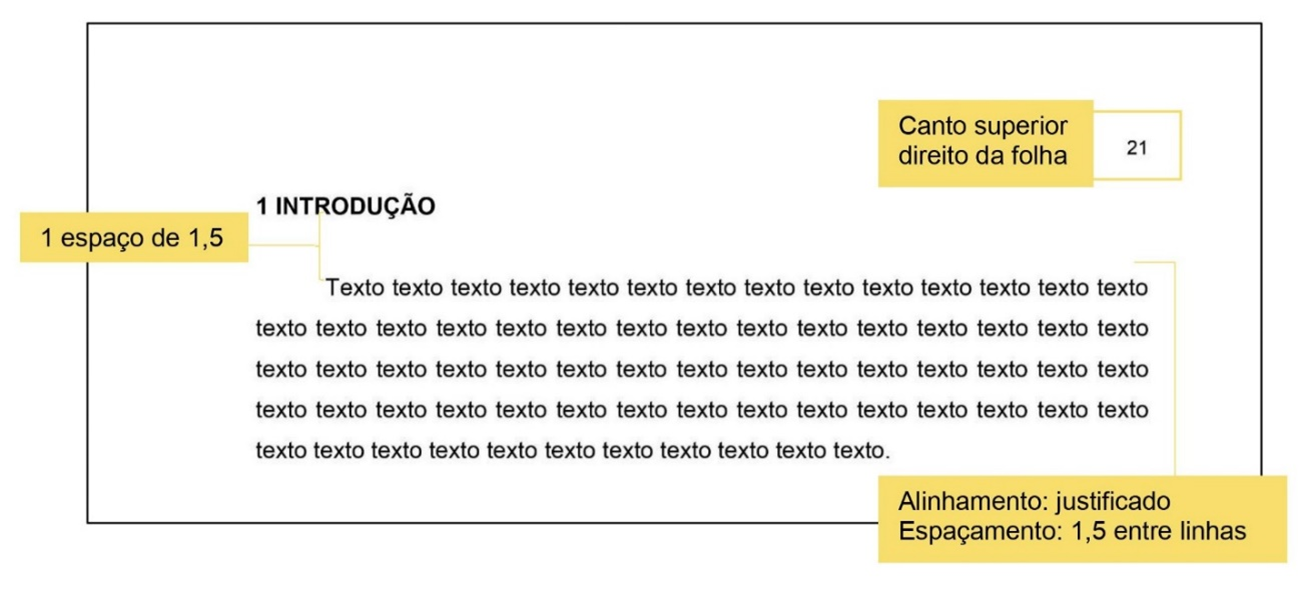
\includegraphics[scale=1]{Textuais/Picture1.png}
	\fonte{Elaborada pelos autores (2020), com base na NBR 14724 (2011).}
\end{figure}


\subsubsubsection{Seção quinaria}



O vídeo fornece uma maneira poderosa de ajudá-lo a provar seu argumento. Ao clicar em Vídeo Online, você pode colar o código de inserção do vídeo que deseja adicionar. Você também pode digitar uma palavra-chave para pesquisar online o vídeo mais adequado ao seu documento. Para dar ao documento uma aparência profissional, o Word\footnote{O Microsoft Word é um processador de texto produzido pela Microsoft Office foi criado por Richard Brodie para computadores IBM PC com o sistema operacional DOS em 1983.} fornece designs de cabeçalho, rodapé, folha de rosto e caixa de texto que se complementam entre si. Por exemplo, você pode adicionar uma folha de rosto, um cabeçalho e uma barra lateral correspondentes.

\begin{table}[!htbp]
	\centering
	%	\small
	\renewcommand{\arraystretch}{1.1}
	\caption{Modelo de tabela.}%
	\label{tab:tabela_exemplo}
	\begin{tabular}{ L{4cm}  R{3cm} || L{4cm}  R{3cm}  }
		\hline
		Município		& População Estimada & Município		& População Estimada 		\\ 
		\hline
		Abdon Batista		& 2630	& Bom Jesus				& 2821 \\ 
		Abelardo Luz		& 17717	& Bom Jesus do Oeste	& 2156 \\ 
		Agrolândia			& 10272	& Bom Retiro			& 9598 \\ 
		Agronômica			& 5306	& Bombinhas				& 17477 \\ 
		Água Doce			& 7132	& Botuverá				& 4943 \\ 
		Águas de Chapecó	& 6379	& Braço do Norte		& 31765 \\ 
		\hline
	\end{tabular}
	\vspace{2mm}
	\fonte{Adaptado de IBGE (2015).}
\end{table}

Clique em Inserir e escolha os elementos desejados nas diferentes galerias.

\begin{figure}
	\centering
	\caption{População.}
	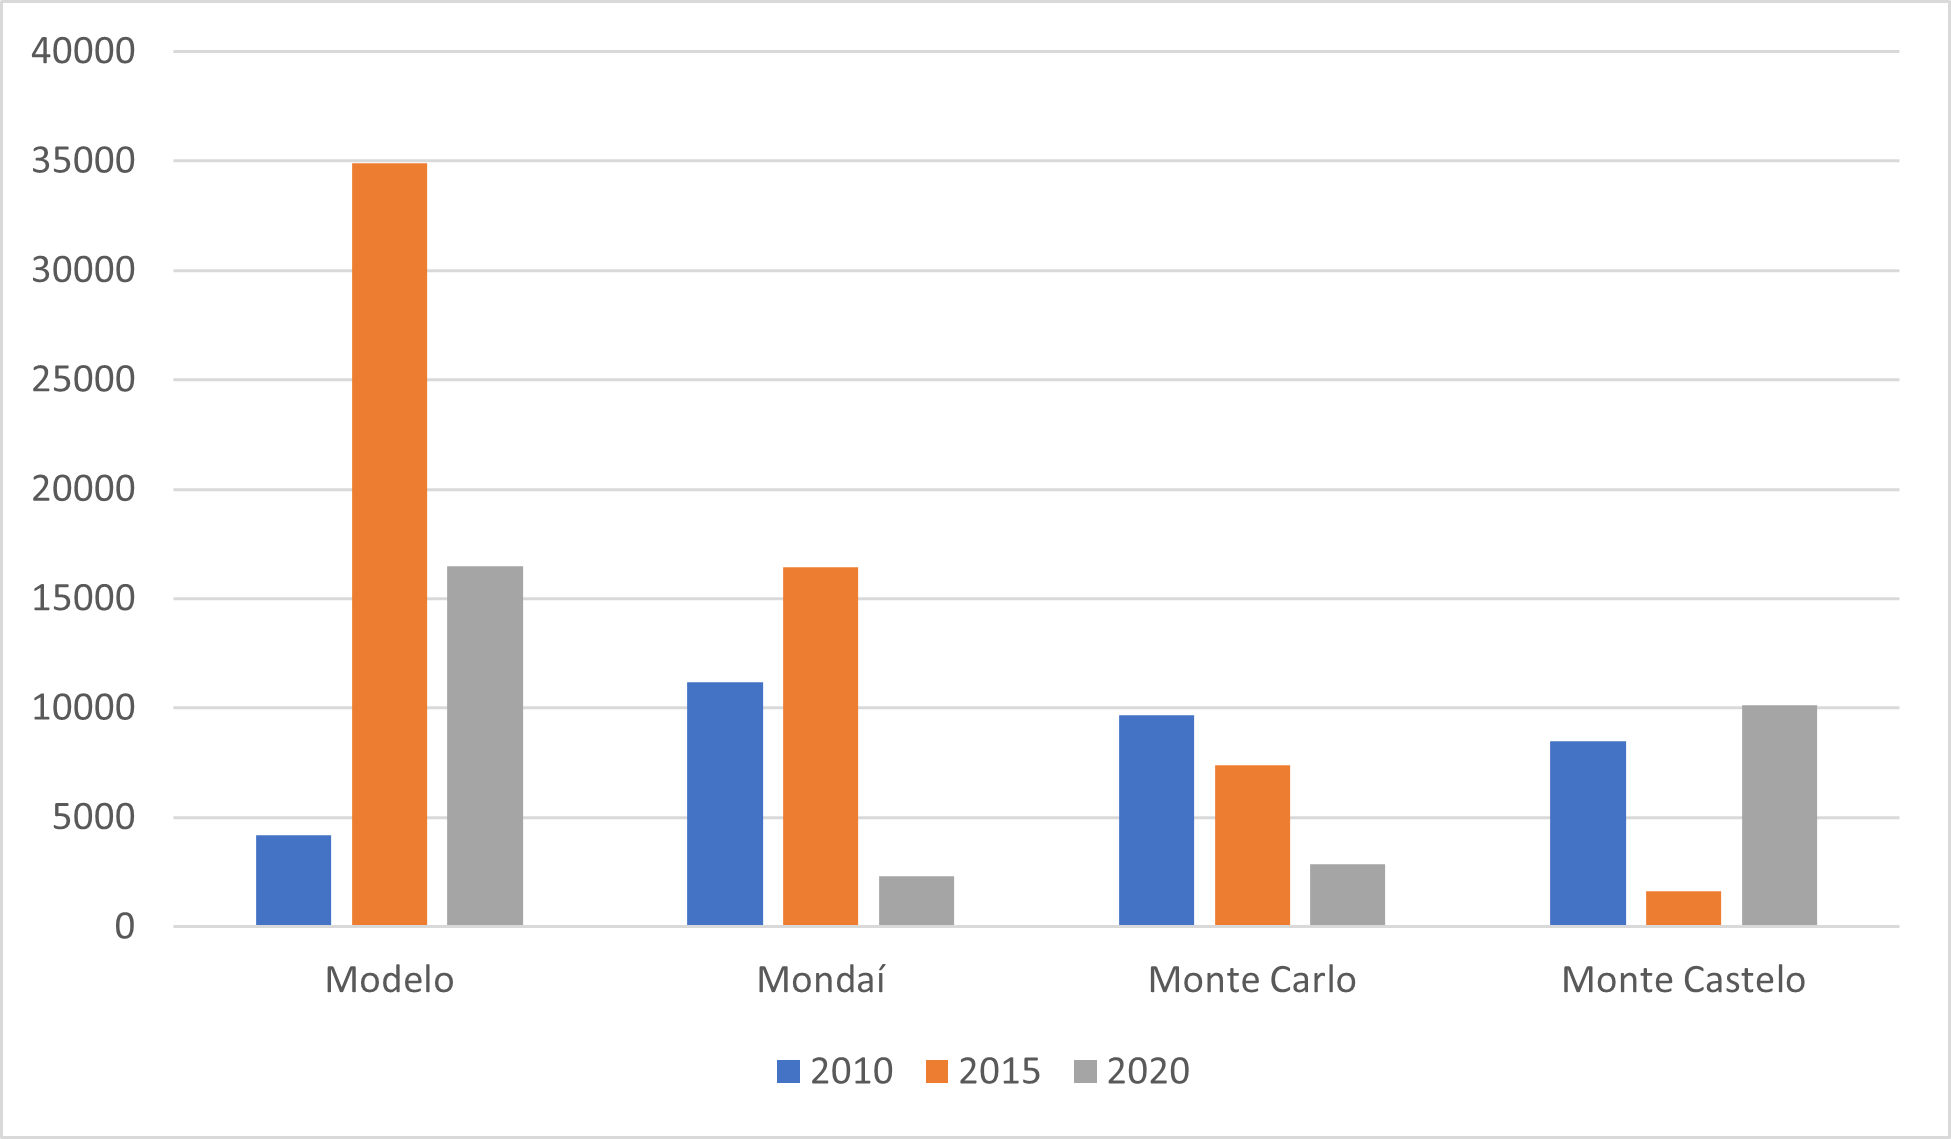
\includegraphics[scale=1]{Textuais/Picture2.png}
	\fonte{\me{2020}}
\end{figure}

As chamadas às equações e fórmulas, no texto, devem ser feitas da seguinte forma: equação (1), fórmula (2).

\textbf{Exemplo 1:}
O Teorema de Pitágoras, é uma equação \eqref{eq:eq1} que pode ser aplicada em qualquer triângulo retângulo (triângulo que tem um ângulo de 90°).
\begin{equation} \label{eq:eq1}
a^2 + b^2 = c^2 
\end{equation}

\textbf{Exemplo 2:}
A dopamina é um composto orgânico de função mista álcool, fenol e amina que apresenta fórmula \eqref{eq:form1} molecular:
\begin{equation} \label{eq:form1}
\ch{C8 + H11NO2} 
\end{equation}

\textbf{Exemplo 3:}
O modelo matemático de Huang (HUG), dado pelas equações \eqref{eq:eq3} e \eqref{eq:eq4}, foi elaborado com o intuito de fornecer uma descrição mais simples do crescimento bacteriano.
\begin{gather} 
	y(t) = y_0 + y_{max} -\ln{[e^{y_0}  + (e^{y_{max}} -e^{y_0} )  e^{-u_{max}\beta(t)} ]}   \label{eq:eq3}  \\
	\beta(t) = t + \frac{1}{4}\ln\left( \frac{1+ e^{-4(t-\lambda)} }{1+ e^{4(\lambda)} }\right) \label{eq:eq4}
\end{gather}
\noindent onde $y(t)$ corresponde ao logaritmo natural da concentração celular (log UFC/g) no instante $t$ (dias), $y_{max}$ é o logaritmo natural da população bacteriana (log UFC/g) final, $y_0$ corresponde ao logaritmo natural da população bacteriana inicial (log UFC/g) e $\beta(t)$ é a função de transição.

\textbf{Exemplo 4:}
Para o cálculo da intensidade fórmula \eqref{eq:eq5} de Intensidade-Duração-Frequência apresentada, os valores encontrados seguindo os parâmetros apresentados e como o resultado é dado em mm/h haverá também a sua conversão para m/s.
\begin{gather} 
	i = \frac{K T^m}{(t+b)^n}   \label{eq:eq5}  \\[2ex]
		i = \frac{\num{625.58} \cdot 5^{\num{0.171}}  }{(60+\num{8.89})^{\num{0.961}}} \\[2ex]
		i = \num{44.222} \cdot \frac{\si{mm}}{\si{h}} \cdot \frac{1\mathrm{m}}{\SI{1000}{mm}} \cdot \frac{\SI{1}{h}}{\SI{3600}{s}} 	
\end{gather}
\noindent onde, $i$ é a intensidade média máxima de precipitação, em mm/h; $T$ é o Período de retorno, em anos; $t$ é a duração da chuva, em minutos; $k,m,b,n$ são os parâmetros da equação determinados para cada local.


As citações diretas com até três linhas ``[...] devem estar contidas entre aspas duplas. As aspas simples são utilizadas para indicar citação no interior da citação.'' (ABNT, 2002, p. 2). Devem apresentar autor, ano e página. Quando a indicação de autor estiver dentro de parênteses, o sobrenome deve ser em letra maiúscula. 


As citações diretas com mais três linhas ``[...] devem ser destacadas com recuo de 4 cm da margem esquerda, com letra menor que a do texto utilizado e sem as aspas.'' (ABNT, 2002, p. 2). Ou seja, utilizar fonte tamanho 10 para as citações diretas longas, com espaçamentos simples entre linhas. As citações devem ser precedidas e antecedidas por um (1) espaço de 1,5 entrelinhas. 

\begin{citacao}
Texto texto texto texto texto texto texto texto texto texto texto texto texto texto texto texto texto texto texto texto texto texto texto texto texto texto texto texto texto texto texto texto texto texto texto texto texto texto texto texto texto texto texto texto texto texto. (SILVA, 2020, p. 21).
\end{citacao}


Nas citações indiretas não há necessidade de usar aspas e indicar a página, considerando que é uma paráfrase. Faz-se necessário apresentar o autor e ano.






\noindent Exemplo referência de livro: \cite{exemplo_livro}

\noindent Exemplo referência de livro em meio eletrônico: \cite{exemplo_livroe}

\noindent Exemplo referência de trabalho acadêmico (Dissertação de Mestrado): \cite{exemplo_dissertacao}

\noindent Exemplo referência de trabalho acadêmico (Tese de Doutorado): \cite{exemplo_tese}

\noindent Exemplo referência de artigo: \cite{exemplo_artigo}


\textbf{Para outras referências ver Manual Udesc}: \url{https://www.udesc.br/bu/manuais}









%


\chapter{Desenvolvimento}







%

\chapter{Conclusão}




\chapter{Introdução}\label{cap:Introducao}
% No presente capítulo apresenta-se a definição do problema, a justificativa para o estudo, os objetivos gerais e específicos, a metodologia utilizada e a estruturação.

% \section{Definição do Problema}\label{sec:DefinicaoProblema}


%A mudança das tecnologias traz uma grande demanda de profissionais das Áreas de ciência, tecnologia, engenharia e matemática, do inglês \textit{science, technology, engineering and mathematics} (STEM).

%Como área de tecnologia, entende-se ciência, tecnologia, engenharia e matemática, do inglês \textit{science, technology, engineering and mathematics} (STEM) e 
%ta quasw

A participação feminina e a evasão escolar nos cursos de graduação em  ciência, tecnologia, engenharia e matemática, do inglês \textit{Science, Technology, Engineering and Mathematics} (STEM) são um problema mundial e historicamente conhecidos. 

% Até início do século XX a presença feminina era considerada indesejada nas universidades \cite{barros:2020}.

A partir disso, a Organização das Nações Unidas (ONU) definiu dentro de seus pilares o quinto Objetivo de Desenvolvimento Sustentável, a inclusão de mulheres nas áreas de STEM a partir da igualdade de gênero.
Apesar das mulheres terem alcançado maior escolaridade que os homens a nível mundial e também dos esforços significativos com as iniciativas públicas, privadas e da sociedade civil para a equidade de gênero, a ONU relata que a maior parte das mulheres está fora da carreira das STEM e com  remunerações inferiores. Em números, a América Latina está melhor representada, 45,1\% de trabalhadores nas STEM são mulheres \cite{unesco:2019}, porém o mesmo não ocorre no Brasil, onde apenas 24\% dos trabalhadores são mulheres desta área \cite{fernandes:2021}. 

Como combate as desigualdades, a inclusão de mulheres nas STEM constitui um dos pilares da ONU para o objetivo número 5 da igualdade de gênero, pois apesar da maior escolaridade comparada a dos homens, elas ainda recebem menores salários no mercado de trabalho. E mesmo quando as mulheres escolhem a carreira das STEM continuam com menores remunerações para os mesmos cargos.

As motivações para essa desigualdade são muitas vezes culturais, como relata \citeonline{alfred:2019} que expõem o senso comum de que mulheres não tem aptidão para as ciências duras, principalmente ciência da computação e as engenharias. Na mesma pesquisa, relata-se que no caso de alunas negras a discriminação institucional acontece ao longo de toda a vida, com punições disciplinares, notas menores e maiores evasões acadêmicas.

\citeonline{natansohn:2021} apresentam que a diversidade no meio das STEM é papel importante, e sua falta, não apenas de gênero, mas também em um contexto das diversidades sociais tornam o ambiente desfavorável a serem ocupados por grupos subalternizados, como mulheres negras, indígenas e a comunidade LGBTQIA+.


No Brasil, o combate a esta desigualdade não parte da legislação, como aponta \citeonline{iwamoto:2022}, que mostra que estes incentivos da inclusão de cidadãos nas STEM é escasso e no caso da inclusão de mulheres é raríssimo. Ao mesmo tempo, a mesma autora aponta diversos projetos internacionais e nacionais, geralmente provindos pela academia para este incentivo.

O desenvolvimento do país está diretamente ligado a esta diversidade que se dá inicialmente com a presença feminina nas universidades e nos cursos das STEM, como aponta \citeonline{lee:2010}, que afirma que a democratização da educação e a inclusão das mulheres na STEM foi a principal fonte para o desenvolvimento da Coreia do Sul a partir da década de 1960.

Com o exposto, entende-se que o combate a desigualdade feminina nas STEM, de maneira geral, inicia-se com sua presença nas universidades e estudar, expor e analisar os fatores que acercam é uma necessidade.

Dada a relevância da análise da presença de mulheres nos cursos das STEM, o presente trabalho busca compreender e analisar a presença de mulheres nos cursos de computação e tecnologia de informação relacionando com os programas de incentivo a sua permanência ou ingresso nas universidades, neste caso o programa Meninas Digitais que será melhor apresentado na Seção \ref{sec:ProjetosLevantados}.

É importante ressaltar que a análise de gênero presente nessa dissertação é relacionada apenas com a classificação dos dados do Instituto Nacional de Estudos e Pesquisas Educacionais Anísio Teixeira (INEP), que não levam em conta a diversidade e pluralidade dos gêneros e optam por classificações binárias.



%o autor tal argumenta...

%Dada a relevância da análise da presença de mulheres nos cursos de Computação e Tecnologias da Informação e Comunicação%...

%\section{Questões de pesquisa}

\section{Justificativa}\label{sec:Justificativa}

A presença de mulheres e a diversidade de gênero nos cursos de Computação e Tecnologia da Informação e Comunicação segundo \citeonline{sbc:2021} são a tradução do que é o desenvolvimento sustentável, criativo e eficiente.
\citeonline{sbc:2021} também apontam sete
motivos (chamados de 7P’s) para promoção da presença diversa no meio da Computação e Tecnologias da Informação e Comunicação (TIC). Produtividade, Pioneirismo, Pertencimento, Parceria, Praticidade, Pluralidade e Persistência. No entanto apenas a equidade de gênero não é suficiente para trazer inovações e descobertas científicas coletivas, é necessário também implantar políticas efetivas e cuidadosamente pensadas.%MAIS DETALHES ** 

Com isso, a contribuição científica que se busca com esta pesquisa está na compreensão do cenário da presença das mulheres nos cursos de TIC e suas relações com os projetos de incentivo a permanência, trazendo um levantamento de iniciativas dos projetos do programa Meninas Digitais da Sociedade Brasileira de Computação.


%====LU NAO GOSTOU===
%Conforme exposto no Capítulo \ref{cap:Introducao}, nota-se que a evasão é diretamente ligada com a permanência nas universidades e quando analisa-se algum desses fatores é imprescindível observar o outro.  %confuso

%A realidade da evasão escolar no Brasil é abordada por diversos autores, bem como a participação das mulheres nos cursos das STEM, como descrito no Capítulo \ref{cap:FundamentacaoTeorica}. Também sabe-se que os incentivos a sua permanência ou ingresso nos cursos desta área não partem da legislação do país e geralmente contam com iniciativas provindas das próprias universidades. 

%Com isso, busca-se aqui compreender e analisar algumas destas iniciativas, trazendo assim sua devida importância, para que sirva de incentivo ou aprendizado para outros projetos e programas como o Meninas Digitais.
%====LU NAO GOSTOU FIM===


%Por isso esse trabalho 

%\section{Hipóteses}
%apenas para não esquecer...
%Será que pode ter um reflexo nas taxas de evasão pelo fato de ter um projeto?

\section{Objetivos}\label{sec:Objetivos}

Para organização do trabalho foram levantados objetivos gerais e específicos e estão apresentados nesta seção.

\subsection{Objetivo Geral}\label{sec:ObjGeral}
Analisar a presença das mulheres nos cursos de Computação e Tecnologias da Informação e Comunicação em universidades brasileiras e sua possível relação com as ações dos projetos parceiros do programa Meninas Digitais.

\subsection{Objetivos Específicos}\label{sec:ObjEspecifico}
Para alcançar o objetivo geral, tem-se como objetivos específicos:
\begin{itemize}

\item Investigar a questão da evasão e sua relação com gênero;

%\item Investigar a participação de mulheres na área das STEM para obter um panorama geral do tema;

\item Explorar as ações realizadas para diminuir a evasão das mulheres na área das STEM;

%\item Investigar os projetos brasileiros de incentivo a participação e presença de mulheres na área das STEM a fim de encontrar um programa estável;

\item Realizar um Mapeamento Sistemático da Literatura sobre evasão escolar;

\item Coletar e processar bases de dados relacionadas a evasão e gênero;

\item Entrevistar pessoas dos projetos parceiros do programa Meninas Digitais para coleta de dados.


%\item Coleta de dados por meio de entrevistas com pessoas dos projetos parceiros do programa Meninas Digitais;

%\item Analisar por frentes distintas a presença e evasão das mulheres nos cursos de TIC que possam ser afetadas por algum dos projetos de incentivo elencados;

%\item Investigar dentro dos projetos de incentivo elencados quais são suas principais iniciativas e frentes de trabalho;

%\item Aplicar e avaliar questionário com os projetos de incentivo elencados;

%\item Levantar todos os cursos de Computação e Tecnologias da Informação e Comunicação nas universidades públicas brasileiras;

%\item Analisar quais destes cursos brasileiros estão cadastrados no programa Meninas Digitais da Sociedade Brasileira de Computação;

%Identificar dez dos projetos cadastrados no programa Meninas Digitais que possuem as menores taxas de evasão escolar e maior presença feminina de acordo com os dados do INEP.

%\item Identificar dez cursos cadastrados no programa Meninas Digitais que possuem as menores taxas de evasão escolar e maior presença feminina de acordo com os dados do INEP.

%\item Análises gráficas sobre o corpo discente e docente, utilizando os dados do INEP dos dez cursos escolhidos;

%Dos dez cursos escolhidos, identificar a representatividade feminina do corpo docente;
%Analisar a partir de gráficos comparativos os  projetos selecionados de acordo com o primeiro objetivo;

%\item Aplicar questionário com mulheres participantes dos dez cursos escolhidos;

%\item Identificar ações de melhoria e padrões de atividades abordadas em cada projeto;
\end{itemize}

\section{Metodologia}\label{sec:Metodologia}
A presente pesquisa é classificada como quali-quantitativa, método misto que segundo \citeonline{creswell:2016} é definido como um
procedimento de coleta, análise e combinação de técnicas quantitativas e qualitativas em um mesmo desenho de pesquisa. A escolha deste método se dá pois a interação do qualitativo e do quantitativo traz mais possibilidades analíticas. O presente trabalho adota a definição de métodos mistos proposta por \citeonline{johnson:2004} que diz que tais métodos são “a classe de pesquisa em que o pesquisador mistura ou combina técnicas de pesquisa quantitativa e qualitativa, métodos, abordagens, conceitos ou linguagem em um único estudo” (JOHNSON; ONWUEGBUZIE, 2004: 17, tradução nossa).

Para a etapa de identificação e exploração do problema foi utilizado o procedimento metodológico de pesquisa bibliográfica para a estruturação dos conceitos e para obter uma visão geral da área.

Em seguida, para entendimento do cenário e estado da arte da predição da evasão escolar foi realizado um Mapeamento Sistemático da Literatura (MSL) que utilizou as diretrizes de \citeonline{petersen:2015}. 

Com o mapeamento ainda em andamento observou-se que havia a necessidade de um passo atrás. Observar não mais a predição da evasão escolar, mas sim as relações da evasão escolar com o engajamento e participação dos estudantes em projetos extracurriculares ou programas de incentivo a permanência. Momento em que a relação de evasão, gênero e programas de incentivo se relacionam e trazem a pesquisa este novo olhar, buscando por meio de análises quantitativas entendimento dos dados do INEP sobre essas perspectivas. 

Após as análises, por meio de entrevistas com os projetos selecionados busca-se encontrar as iniciativas realizadas, casos de sucesso e processos de abordagem para incentivo a permanência de mulheres na área da Computação e Tecnologias da Informação e Comunicação.

E por fim, analisar as possíveis relações entre a evasão ou permanência de mulheres nos cursos de TIC com o Programa Meninas Digitais. 

%XX, pois sua principal característica XXX.
%A primeira etapa consistiu em....
%Em seguida realizou-se um Mapeamento Sistemático da literatura, a fim de identificar melhor o campo de trabalho sobre a evasão, observando como é classificada e em quais contextos educacionais é mais observada.



\section{Organização do Texto}\label{sec:Estrutura}
A organização da pesquisa se dá em forma de capítulos e inicia com a fundamentação teórica, que visa descrever os principais tópicos do Capítulo \ref{cap:FundamentacaoTeorica} que são evasão escolar, dados do INEP e suas classificações, a participação de mulheres nas STEM e o cálculo da evasão escolar.

No Capítulo \ref{cap:trabRelacionados} apresentam-se os trabalhos relacionados a esta dissertação. Os trabalhos apresentados relacionaram intervenções ou projetos, como o Meninas Digitais a dados educacionais, como a nota dos estudantes, perfil e participação e apresentam propostas para amenizar a evasão ou aumentar a permanência de estudantes da área das STEM, em específico mulheres.

No Capítulo \ref{cap:Desenvolvimento} é apresentado o processo de pesquisa, onde inicialmente foi desenvolvido um Mapeamento Sistemático da Literatura para compreensão da evasão e dos algoritmos para sua predição e em seguida foi dado um passo atrás e se inicia o entendimento dos dados escolares do INEP relacionando-os com o Programa Meninas Digitais. Nesta etapa os dados são explorados e analisados a partir de gráficos e tabelas. Propõe-se também realização de entrevistas com as pessoas de projetos parceiros do Programa Meninas Digitais escolhidos para melhor entendimento das propostas, colaborações e incentivos a permanência de mulheres nos cursos de Computação e Tecnologias da Informação e Comunicação.

O Capítulo \ref{cap:Consideracoes} apresenta um cronograma de atividades e os resultados parciais deste trabalho.



\chapter{Fundamentação Teórica}\label{cap:FundamentacaoTeorica}

A fundamentação teórica visa abordar os principais assuntos relacionados a proposta de pesquisa. Na primeira Seção \ref{sec:ConceitosEvasao} é introduzido cronologicamente os conceitos de evasão escolar. Com os conceitos apresentados, é definido qual conceito é utilizado neste trabalho para que na seção \ref{sec:ClassificacaoDados} sejam apresentados os dados educacionais da base do INEP  e suas classificações. 

Na Seção \ref{sec:MeninasDigitais} apresenta-se o cenário da participação das mulheres na área das STEM. A seção \ref{sec:CalculoEvasao} une os conceitos anteriores ao cálculo da Evasão, relacionando com as variáveis da base de dados. E por fim, a Seção \ref{sec:discussaoCapitulo} encerra o capítulo com uma discussão e geral sobre as seções anteriores.


\section{Evasão Escolar}\label{sec:ConceitosEvasao}
A permanência no ensino superior está diretamente ligada a evasão escolar, para isso, faz-se necessário trazer análises relacionadas a evasão das mulheres, especificamente nos cursos de Computação e Tecnologia da Informação, mas antes disso é importante conceituar a evasão.

Apesar do conceito de evasão parecer autoexplicativo e entendido como a saída do estudante do curso antes da obtenção do diploma, não há um consenso no termo evasão. %As próximas subseções apresentam esses conceitos e também as formas de se calcular a evasão.

%Sabe-se que a evasão é um tema complexo e nessa subseção aborda-se os diferentes conceitos, além de apresentar o conceito utilizado nesse trabalho.

O INEP conceitua evasão e diferencia do termo abandono, "O conceito técnico de abandono é diferente de evasão. Abandono quer dizer que o aluno deixa a escola num ano mas retorna no ano seguinte. Evasão significa que o aluno sai da escola e não volta mais para o sistema" \cite{estatistica:2014}.

\citeonline{utiyama:2003} abordam a evasão diretamente como a saída definitiva do aluno de seu curso de origem, sem concluí-lo. Não estabelece critérios de tempo de curso, momento da saída e nenhuma outra variável relacionada. Já \citeonline{fernandes:2005} define evasão como os alunos que não completaram cursos ou programas de estudo e diferente dos outros conceitos, especifica que deve-se considerar nos cálculos os alunos que nunca iniciaram o curso, mas se matricularam. 

\citeonline{gaioso:2005} apresenta como definição de evasão “interrupção no ciclo de estudo” e segundo a autora isso ocorre quando o aluno deixa o curso por qualquer motivo diferente da conclusão e obtenção da titulação. O trabalho de \citeonline{gaioso:2005} também apresenta os motivos pelos quais o aluno é classificado como evadido, sendo eles não efetuar a matrícula no prazo estabelecido, transferência interna ou mudança de curso, transferência externa, matrícula em curso de outra instituição via aprovação em processo seletivo, desistência, re-opção ou jubilamento.

\citeonline{abbad:2006} referem-se a evasão como a desistência definitiva do aluno em qualquer etapa do curso, porém não deixam claro se aplica-se também aos alunos que apenas se matricularam e nunca iniciaram o curso de fato.


Com apresentado, existe uma série de definições para o termo evasão, no presente estudo, consideram-se evadidos todos os alunos desistentes com algum vínculo de matrícula, mesmo nunca tendo assistido a uma aula. Tal abordagem é utilizada por tratarmos aqui com dados provindos do INEP, onde essa distinção não é apresentada. Conhecer bem o fenômeno de evasão tem papel fundamental para a promoção de ações adequadas.

Nesta dissertação, o conceito utilizado é a evasão de curso, pois pretende-se entender a evasão feminina dos cursos de Computação e Tecnologias da Informação e Comunicação, mesmo que a aluna tenha permanecido na mesma instituição de ensino superior fazendo outro curso ou se foi transferida para o mesmo curso em outra instituição.



\section{Dados do INEP e suas classificações} \label{sec:ClassificacaoDados}%suas classificações são as classificações de cada coluna utilizada, como por ex o número 06 do CINE (Classificação Internacional Normalizada da Educação)

A grande maioria dos estudos e dados estatísticos relacionados aos níveis da educação brasileira são fornecidos pelo Instituto Nacional de Estudos e Pesquisas Educacionais Anísio Teixeira (INEP), que é classificado como uma autarquia federal e está vinculado ao Ministério da Educação (MEC). Tais estudos e dados são realizados e fornecidos com o principal objetivo de auxiliar o desenvolvimento educacional, econômico e social do país, realizando o desenvolvimento de iniciativas e políticas educacionais para contribuir com todas essas áreas da sociedade.

Uma das principais ações que o INEP realiza, é a divulgação e disponibilização anual dos microdados do Censos da educação básica até a educação superior, assim oferecendo diversos dados estatísticos que possibilitam a realização de estudos, desenvolvimento de ferramentas e técnicas para contribuição com as gestões públicas educacionais. Segundo \citeonline{ferreira:2021}, é importante a atualização e disponibilização anual dessas bases de dados, pois suas informações podem ajudar a melhorar e também resolver os problemas presentes em nosso sistema de educação.


Observando a organização de dados apresentadas na base, para que as publicações dos dados estatísticos educacionais seguissem os parâmetros utilizados internacionalmente em pesquisas relacionadas à educação, o INEP passou a adotar o chamado \textit{International Standard Classification of Education} (ISCED), que traduzido para o português significa Classificação Internacional Normalizada da Educação (CINE). A ISCED é a referência proposta pela Unesco para classificar cursos e certificações seguindo um padrão que permite reunir, compilar e analisar estatísticas educacionais comparáveis tanto ao âmbito nacional como internacional (Unesco, 2015).

Essa mudança adotada pelo INEP, resultou na CINE Brasil, que corresponde a Classificação Internacional Normalizada da Educação adaptada para os cursos de graduação presentes no Brasil. A CINE Brasil consiste em 11 áreas de formação, as quais são classificadas como segue: 00 Programas Básicos; 01 Educação; 02 Artes e Humanidades; 03 Ciências Sociais, Comunicação e Informação; 04 Negócios, Administração e Direito; 05 Ciências Naturais, Matemática e Estatística; 06 Computação e Tecnologias da Informação e Comunicação (TIC); 07 Engenharia, Produção e Construção; 08 Agricultura, Silvicultura, Pesca e Veterinária; 09 Saúde e Bem-Estar e 10 Serviços. 

Esta classificação de cursos 06 Computação e Tecnologias da Informação e Comunicação (TIC) abrangem as formações relacionadas a gestão de TIC, produção de software, ciência da computação, sistemas de informação, engenharia de computação, soluções computacionais para domínios específicos, bem como formações interdisciplinares que apresentem como principal conteúdo Computação e Tecnologias da Informação e Comunicação (TIC). Quanto a engenharia de computação, ela pode ser classificada como 06 ou como 07, que é específico para as engenharias, isso depende de qual resolução do Ministério da Educação (MEC) que o curso segue.

Ao relacionar a classificação CINE com o banco de dados do INEP dos anos de 2009 até 2019 obtém-se um total de 465 nomes de cursos em todo o Brasil. No mesmo contexto brasileiro, existem 24.858 cursos classificados como 06. A Tabela \ref{tab:QtdCursos} apresenta o agrupamento dos 20 nomes de cursos mais usados (93,6\%). É possível observar pela Tabela \ref{tab:QtdCursos}, que o nome Ciência da Computação aparece com acento na terceira linha (n=3491), sem acento na décima terceira linha (n=281) e no plural na décima sétima linha (n=126). Desta forma percebe-se a não padronização dos dados.


\begin{table}[H]
\centering
\caption{Quantidade por Nome de Curso de 2009 a 2019}
\label{tab:QtdCursos}
\resizebox{\textwidth}{!}{%
\begin{tabular}{|l|r|}
\hline
\rowcolor[HTML]{C0C0C0} 
{\color[HTML]{000000} NOME CURSO}                                                                                                      & \multicolumn{1}{l|}{\cellcolor[HTML]{C0C0C0}{\color[HTML]{000000} QUANTIDADE DE CURSOS}} \\ \hline
{\color[HTML]{000000} ANÁLISE E DESENVOLVIMENTO DE SISTEMAS}                                                                           & {\color[HTML]{000000} 4823}                                                              \\ \hline
{\color[HTML]{000000} SISTEMAS DE INFORMAÇÃO}                                                                                          & {\color[HTML]{000000} 4320}                                                              \\ \hline
{\color[HTML]{000000} CIÊNCIA DA COMPUTAÇÃO}                                                                                           & {\color[HTML]{000000} 3491}                                                              \\ \hline
{\color[HTML]{000000} REDES DE COMPUTADORES}                                                                                           & {\color[HTML]{000000} 2585}                                                              \\ \hline
{\color[HTML]{000000} SISTEMA DE INFORMAÇÃO}                                                                                           & {\color[HTML]{000000} 1678}                                                              \\ \hline
{\color[HTML]{000000} GESTÃO DA TECNOLOGIA DA INFORMAÇÃO}                                                                              & {\color[HTML]{000000} 1658}                                                              \\ \hline
{\color[HTML]{000000} SISTEMAS PARA INTERNET}                                                                                          & {\color[HTML]{000000} 1311}                                                              \\ \hline
{\color[HTML]{000000} JOGOS DIGITAIS}                                                                                                  & {\color[HTML]{000000} 580}                                                               \\ \hline
{\color[HTML]{000000} ENGENHARIA DE COMPUTAÇÃO}                                                                                        & {\color[HTML]{000000} 512}                                                               \\ \hline
{\color[HTML]{000000} SISTEMAS DE INFORMACAO}                                                                                          & {\color[HTML]{000000} 496}                                                               \\ \hline
{\color[HTML]{000000} CIENCIA DA COMPUTACAO}                                                                                           & {\color[HTML]{000000} 281}                                                               \\ \hline
{\color[HTML]{000000} BANCO DE DADOS}                                                                                                  & {\color[HTML]{000000} 274}                                                               \\ \hline
{\color[HTML]{000000} ENGENHARIA DE SOFTWARE}                                                                                          & {\color[HTML]{000000} 258}                                                               \\ \hline
{\color[HTML]{000000} SEGURANÇA DA INFORMAÇÃO}                                                                                         & {\color[HTML]{000000} 247}                                                               \\ \hline
{\color[HTML]{000000} INFORMÁTICA}                                                                                                     & {\color[HTML]{000000} 186}                                                               \\ \hline
{\color[HTML]{000000} \begin{tabular}[c]{@{}l@{}}CURSO SUPERIOR DE TECNOLOGIA EM\\ ANALISE E DESENVOLVIMENTO DE SISTEMAS\end{tabular}} & {\color[HTML]{000000} 151}                                                               \\ \hline
{\color[HTML]{000000} CIÊNCIAS DA COMPUTAÇÃO}                                                                                          & {\color[HTML]{000000} 126}                                                               \\ \hline
{\color[HTML]{000000} ENGENHARIA DA COMPUTAÇÃO}                                                                                        & {\color[HTML]{000000} 108}                                                               \\ \hline
{\color[HTML]{000000} PROCESSAMENTO DE DADOS}                                                                                          & {\color[HTML]{000000} 105}                                                               \\ \hline
{\color[HTML]{000000} \begin{tabular}[c]{@{}l@{}}CURSO SUPERIOR DE TECNOLOGIA EM \\ REDES DE COMPUTADORES\end{tabular}}                & {\color[HTML]{000000} 81}                                                                \\ \hline
\end{tabular}%
}
\end{table}

%Com essa classificação entende-se melhor a pluralidade dos cursos. Uma base de dados muito rica é apresentada no censo escolar dos anos de 2009 a 2019. 

Além das classificações CINE, os dados do INEP funcionam principalmente a partir de códigos e para melhor entendimento de sua base deixam disponível um dicionário de variáveis. O dicionário apresenta 105 variáveis distintas, que estão divididas em categorias, sendo elas dados da Instituição de Ensino Superior (IES), dados do curso, dados do aluno e variáveis derivadas.

É importante ressaltar que para a busca de curso e IES específicas a base do INEP utiliza-se dos códigos gerados pelo e-MEC\footnote{http://emec.mec.gov.br/}, que é o sistema eletrônico de acompanhamento dos processos que regulam a educação superior no Brasil. 

\section{Participação de Mulheres nas STEM}\label{sec:MeninasDigitais}
%meninas digitais
%https://www.sbc.org.br/images/flippingbook/computacaobrasil/computa_44/pdf/CompBrasil_44.pdf

A participação das mulheres em diversos setores foi fator de incomodo para a sociedade, votar, trabalhar e estudar eram tarefas exclusivamente masculinas, isso não foi diferente no setor educacional, segundo \citeonline{barros:2020} até início do século XX a presença feminina  nas universidades era considerada indesejada.

Esta exclusão histórica reflete na baixa participação de mulheres em diversos setores e tal exclusão pode ser dividida em dois tipos a horizontal, que é a falta de  mulheres em áreas específicas
do conhecimento, e a vertical, que é a sub-representação de mulheres em postos de prestígio e poder, mesmo em carreiras consideradas femininas \cite{araujoM:2020}. 

A presença feminina na educação superior brasileira embora seja expressiva de uma maneira geral, como \citeonline{suzane:2018} apresentam em sua pesquisa, em que as mulheres possuem 53,8\% das matrículas nas universidades públicas e 58,6\% nas particulares. Apesar disso, esse cenário não é igualitário em todas as áreas da ciência. A mulher tem uma representatividade minoritária nos cursos da área da computação, \citeonline{marcel:2016} mostra que entre 2000 e 2013, apenas 17\% dos concluintes eram do gênero feminino.

Esse fenômeno se replica também em universidades de outros países, como os Estados Unidos \cite{lunn:2021}. Nos anos 80, 40\% dos diplomas em Ciência da Computação nos Estados Unidos eram de mulheres, ao passo que em 2013, elas representaram somente 18\% dos estudantes graduados, e ainda o curso de Ciência da Computação mostra-se o único curso em que a disparidade de gênero está aumentando nas últimas décadas \cite{NCWIT:2020}.

Incentivar a diversidade de gênero em todas as áreas e em específico na área das STEM, dentro e fora da universidade, segundo \citeonline{sbc:2021} traz benefícios financeiros, criativos, de cooperação e sensação de pertencimento da equipe como um todo. \citeonline{sbc:2021} complementam que ainda temos muito a evoluir em relação à diversidade de gênero e que é esse o momento de buscar incentivos.

\citeonline{oliveira:2019} afirmam que nos últimos anos o Brasil contou com iniciativas que incentivam o ingresso e a permanência de mulheres nas áreas STEM e cita como exemplo as iniciativas do Conselho Nacional
de Desenvolvimento Científico e Tecnológico (CNPq), executadas no âmbito do Programa
Mulher e Ciência\footnote{https://www.gov.br/cnpq/pt-br/acesso-a-informacao/acoes-e-programas/programas/mulher-e-ciencia/mulher-e-ciencia}.

As iniciativas levantadas por \citeonline{oliveira:2019} do programa Mulher e Ciência do CNPQ  tem como objetivo fomentar a pesquisa na temática relações de gênero, mulheres e feminismo, impulsionar a discussão de gênero em todos os níveis educacionais e fomentar a formação de recursos humanos nesta temática, estimular a formação de mulheres para as carreiras de
ciências exatas, engenharias e computação no Brasil e tudo isso por meio de chamadas de apoio a projetos, encontros e prêmios.

No mesmo âmbito de incentivo a participação, permanência e presença de mulheres nas STEM, \citeonline{iwamoto:2022} apresenta em seu trabalho um levantamento de publicações no Diário Oficial da União (DOU) brasileiro envolvendo mulheres nas STEM com o intuito de verificar se as diretrizes nacionais e internacionais estão sendo levadas em conta na instituição de políticas públicas.

\citeonline{iwamoto:2022} fez sua busca em dezembro de 2021 no domínio “in.gov.br” utilizando o portal de busca do \textit{Google}. As palavras-chave utilizadas foram “mulheres STEM” e “mulheres tecnologias” e como retorno obteve 5 resultados para a primeira palavra-chave e 94.500 resultados para a segunda. Fez uma limpeza excluindo artigos que não falavam sobre mulheres nas STEM e também excluiu as portarias relativas a nomeação, remoção e afins. Concluiu que há raras políticas públicas de inclusão de mulheres nas STEM em âmbito federal no Brasil e afirma que este quadro prevê um baixo desenvolvimento no país nos próximos anos.

%Com esse cenário de baixo incentivo a permanência e participação das mulheres, observa-se a evasão escolar ...

%---Finalizar a seção para fazer sentido com a próxima---








 








%Reforçando que o contexto cultural das mulheres não terem aptidão para a área das STEM é equivocado, ....

%USAR ESSE PRA INICIAR AQUI: "Apesar desse efeito visível e concreto no cotidiano das instituições educativas em geral, umestudo da Organização para a Cooperação e Desenvolvimento Econômico (OECD, 2019) sobre oteste Pisa (Programme for International Student Assessment [Programa Internacional de Avaliaçãode Estudantes])" DO ARTIGO MULHERES NAS STEM: UM ESTUDO BRASILEIRO NO DIÁRIO OFICIAL DA UNIÃO. FALA QUE AS MENINAS TIRAM NOTAS BOAS EM CIENCIAS.



\section{Cálculo da Evasão}\label{sec:CalculoEvasao}
%QUAL A DIFERENÇA DELES?
%%%Equação MEC - Pg 22 do pdf http://www.dominiopublico.gov.br/download/texto/me002240.pdf
%Para a construção da equação utilizada nesse trabalho, faz-se importante a contextualização histórica dos cálculos de evasão.
Encontra-se na literatura diversas abordagens para o cálculo da evasão. \citeonline{diplomaccao:1996} trouxe um dos primeiros métodos para chegar a porcentagem de evasão dos cursos superiores, como demonstrado na Equação 1.

\renewcommand{\theequation}{Eq. \arabic{equation}} 
\begin{equation}\label{eq:mec}
E = \frac{Ni - Nd - Nr}{Ni}\times{100}
\end{equation}

Interpretando a Equação 1 tem-se que \textit{Ni} é o número de ingressantes no ano-base e calcula-se a partir da soma do número de diplomados, o número de evadidos e o número de retidos. Essa equação considera a série histórica de dados sobre uma turma de alunos ingressantes e o tempo máximo de integralização curricular, para por fim, serem identificados como evadidos do curso os alunos que não se
diplomaram neste período e que não estão mais vinculados ao curso em questão. 

Diferente das equações seguintes, a Equação 1 é utilizada para acompanhar uma ou mais turmas de determinado curso, calcula-se a evasão levando em conta o ano de ingresso e o tempo máximo para conclusão do curso.
%%%%----FIM MEC


%%%%------silva 2007
Já \citeonline{silva:2007} apresenta o calculo da evasão da seguinte maneira: 

\begin{equation}\label{eq:evasaovelha}
E(n) = 1 - \frac{M(n) - I(n)}{M(n - 1) - C(n - 1)}
\end{equation}


Sendo que \textit{E} é a evasão a ser calculada, \textit{M} é a quantidade de matriculados, \textit{I} é a quantidade de ingressantes, \textit{C} é a quantidade de concluintes, \textit{n} é o ano de referência e \textit{n - 1} é o ano anterior. A proposta de \citeonline{silva:2007} utilizou a base do INEP para realizar seu trabalho. Deve-se ressaltar que \citeonline{silva:2007} analisam os dados dos anos anteriores a 2009, ano em que ocorreu uma mudança na organização dos dados do INEP, logo a Equação 2 não pode ser utilizada em anos posteriores a 2009 com as mesmas variáveis.
%%%%%%%

A mudança na base de dados do INEP que impossibilita o uso das mesmas equações pode ser observada a partir do manual do usuário disponibilizado em cada base, que mostra diferentes variáveis presentes nos anos anteriores a 2009. As diferenças já iniciam na nomenclatura e disposição dos diretórios, onde um padrão é seguido nos anos anteriores a 2008 e outro de 2009 até 2019.

Os dados de 2008 são divididos em:
\begin{itemize}
    \item Graduação Presencial – Contém informações sobre arquivos associados à área de curso de Graduação Presencial, tais como: vagas, ingressantes, inscritos, concluintes e etc;
    \item Graduação à Distância – Contém informações sobre arquivos associados a área de curso de Graduação à Distância;
    \item Forme-Presencial – Contém informações sobre arquivos associados à área de curso de Formação Específica Presencial tais como: vagas, ingressantes, inscritos, concluintes e etc;
    \item Forme-Distância – Contém informações sobre arquivos associados à área de curso de Formação Específica a Distância;
    \item Secomple-Presencial – Contém informações sobre arquivos associados à área de curso de Sequenciais de Complementação de Estudos Presencial tais como: vagas, ingressantes, inscritos, concluintes e etc;
    \item Secomple-Distância – Contém informações sobre arquivos associados à área de curso de Sequenciais de Complementação de Estudos á Distância;
    \item Instituições – Contém informações sobre arquivos associados as IES, tais como: pessoal docente, pessoal técnico administrativo, dados financeiros, infraestrutura e etc.
\end{itemize}
  
Já as bases a partir de 2009 são organizadas em:
\begin{itemize}
    \item SUP\_IES\_2009 - Contém informações sobre as Instituições de Ensino Superior;
    \item SUP\_CURSO\_2009 - Contém informações sobre os cursos oferecidos;
    \item SUP\_DOCENTE\_2009 - Contém informações sobre os docentes;
    \item SUP\_ALUNO\_2009 - Contém informações sobre os alunos;
    \item SUP\_LOCAL\_OFERTA\_2009 - Contém informações sobre o local que a IES se encontra;
    \item TB\_AUX\_CINE\_BRASIL\_2009 - tabela auxiliar dos códigos CINE.
\end{itemize}

Desta forma, percebe-se a grande diferença na organização dos dados a partir de 2009. Observando mais a fundo a discriminação das tabelas dos anos de 2008 e 2009, os dados presentes na base 'Graduação Presencial' de 2008 possui 1.314 colunas, já os itens da base 'SUP\_ALUNO\_2009' de 2009 possui 105 colunas.



%Nesses dois anos em específico, observa-se que em 2008 ainda não utilizava a classificação CINE para os cursos e sim códigos disponibilizados no manual do usuário.

%%%% equação utilizada no trabalho:
Em 2017, a Diretoria de Estatísticas Educacionais publicou a Metodologia de Cálculo dos Indicadores de Fluxo da Educação Superior \citeonline{dados:2017}, onde apresentou uma nova forma de calcular a Taxa de Desistência Anual (Tada), apresentada na Equação 3, e que leva em consideração a organização dos dados do INEP a partir de 2009. É importante salientar que a definição adotada de desistência é a mesma da evasão, sendo utilizados como sinônimos ao longo do documento \citeonline{dados:2017}.

\begin{equation}\label{eq:evasaonova}
{Tada_{j,T,t}} = \frac{\sum_{i=1}^{n_{j,t}} Des_{i,j,t} + \sum_{i=1}^{n_{j,t}} Transf_{i,j,t}} {\sum_{i=1}^{n} IG^T_{i,j} - \sum_{w=T}^{t} \sum_{i=1}^{n_{j,w}} Fal_{i,j,t}} \times{100}
\end{equation}

De acordo com \citeonline{dados:2017}, para encontrar a porcentagem de evasão em determinado período de tempo, assume-se a Equação 3 onde a variável \textit{j} representa a Instituição de Ensino Superior, \textit{t} é o ano de referência, \textit{T} é o ano de ingresso, nota-se que \textit{t} $\geq$ \textit{T}, \textit{Des} representa o estudante com situação de vínculo igual a “Desvinculado do Curso” no curso \textit{j} no ano \textit{t}, \textit{Transf} os estudante com situação de vínculo igual a “Transferido para outro curso da mesma IES” no curso \textit{j} no ano \textit{t}, \textit{IG} o número total de ingressantes no curso \textit{j} no ano \textit{T} e \textit{Fal} estudante com situação de vínculo igual a “Falecido” no curso \textit{j} no ano \textit{t} e no ano \textit{T}. 

Nesse contexto é importante ressaltar que o número total de ingressantes (\textit{IG}) não é representado no banco de dados por uma única variável, e sim pela somatória de diversas variáveis, sendo elas o somatório de: Estudantes com situação de vínculo igual a ``Cursando'', ``Matrícula trancada'', ``Desvinculado do curso'', ``Transferido para outro curso da mesma IES'', ``Formado” e  ``Falecido'' no curso \textit{j} no ano \textit{t} mais os Estudantes com situação de vínculo igual a ``Desvinculado do curso'', ``Transferido para outro curso da mesma IES'', ``Formado'' e  ``Falecido'' no curso \textit{j} no ano \textit{T}.
%%%%%%%---------fim

A Equação 2 se difere da Equação 3 basicamente apenas por suas variáveis, que a partir de 2009 foram modificadas na base do INEP, mas seu objetivo final é o cálculo da evasão anual, observando se o aluno progride de um ano para o posterior, por exemplo, para observar a evasão de determinado curso no ano presente, é necessário observar o ano presente e o ano anterior.

Com o exposto, entende-se que as bases são completamente distintas, observando ainda mais profundamente, os dados de 2008 não contabilizam por exemplo o número de alunos falecidos, o que já inviabiliza a utilização da Equação 3 para os anos anteriores a 2019.

Além das Equações citadas, exitem outras formas de calcular a evasão escolar no ensino superior. \citeonline{antonio:2014} mostra duas equações semelhantes as apresentadas e as compara com a Equação 2 utilizada por \citeonline{silva:2007}. \citeonline{antonio:2014} utiliza de dados simulados e encontra divergência em todos os cálculos, mostrando então a fragilidade e dificuldade de um padrão para o entendimento da evasão. Desta forma, faz-se necessário em todas as publicações explicitar qual modelo foi utilizado. %mais detalhes **


\section{Discussão do Capítulo}\label{sec:discussaoCapitulo}

O presente capitulo abordou na Seção \ref{sec:ConceitosEvasao} os conceitos de evasão no decorrer dos anos e finaliza trazendo o conceito utilizado nesta dissertação que considera os estudantes evadidos como todos os  desistentes com algum vínculo de matrícula, mesmo
nunca tendo assistido a uma aula.Após isso, apresentou a fundamentação dos dados do INEP e suas classificações, onde esclarece quais foram as bases utilizadas e mostra algumas inconsistências nos dados, como a repetição de nome de curso que é encontrada na base do INEP.

É abordado também sobre a participação da mulher na área das STEM, apresentando diversos pontos de vista, brasileiros e internacionais, sobre a presença e evasão das mulheres na área. Para então introduzir sobre como o cálculo da evasão é feito, onde faz-se um levantamento de equações presentes na literatura para por fim escolher a equação que melhor se adéqua aos dados do INEP dos anos anteriores a 2019. 

Com toda fundamentação exposta, uma busca de trabalhos é apresentada no Capítulo \ref{cap:trabRelacionados}
%colocar os principais pontos e fazer ligacoes com o proximo capitulo que sao os trabalhos relacionados **




\chapter{Trabalhos Relacionados}
%%amadurecer e ver o que esses trabalhos se relacionam com o meu trabalho.
\label{cap:trabRelacionados}
Por meio de um levantamento bibliográfico da literatura buscou-se identificar trabalhos relacionados que abordem as áreas  deste trabalho: evasão, programas de incentivo a permanência e aumento da presença feminina nos cursos de Computação e Tecnologias da Informação e Comunicação. 

São descritas ações diversas, a Seção \ref{sec:impulsoparamulheres} apresenta o programa de impulso para mulheres na área da Ciência da Computação, mostrando iniciativas como cursos, grupos de suporte e entre outros que por fim traz números positivos na permanência de mulheres na área. 

A Seção \ref{sec:intervencaoinclusaoretencao} apresenta uma intervenção a fim de amenizar a diferença de gênero no curso de Ciência da Computação. Propõe modificar a forma com que os estudantes recebem suas notas e após essa intervenção apresenta suas descobertas positivas. 

A Seção \ref{sec:meninasuff} apresenta uma iniciativa brasileira de um projeto parceiro do programa Meninas Digitais que propõe uma dinâmica com 37 estudantes e por fim propõe um debate sobre o motivo do baixo número de mulheres na área das TICs.

Na Seção \ref{sec:subareas}, as autoras mostram a relação de gênero e a presença de mulheres dentro das sub-áreas da computação, trazendo assim outra perspectiva da relação de gênero, mesmo assim contribuem para a construção deste trabalho.

O trabalho apresentado na Seção \ref{sec:IniciativasPermanencia} mostra uma revisão sistemática da literatura, que seleciona 73 artigos para encontrar o que a literatura apresenta a respeito de iniciativas educacionais para motivar a permanência das mulheres nas universidades brasileiras nos cursos relacionados à Computação na última década (2010-2019) e como conclusão elenca uma série de iniciativas encontradas.%TERMINAR COM OS OUTROS **

%De acordo com o Censo da Educação Superior de 2015, as mulheres foram a maioria entre as matriculas ativas em cursos da educação superior no Brasil, representando cerca de 55,6\% de todos os estudantes naquele ano. Além disso, também foram a maioria entre os ingressantes (53,9\%) e os concluintes (59,9\%). Porém, ao analisar os cursos escolhidos por homens e mulheres, é notável a diferença entre as áreas escolhidas, pois em sua grande maioria, as mulheres acabam optando por cursos relacionadas ao cuidado, como Pedagogia, Enfermagem e Psicologia, já os homens acabam escolhendo cursos mais relacionados com as áreas tecnológicas, como as Engenharias e os cursos de Computação \cite{moreira:2018}.

\section{Um Impulso para Mulheres na Ciência da Computação}\label{sec:impulsoparamulheres}
Nesta Seção o autor \citeonline{beck:2007} apresenta uma iniciativa que aconteceu em sua Universidade \textit{Truman State}. Tal projeto teve como inspiração outra iniciativa que obteve sucesso na retenção de mulheres na computação: um grupo de suporte para mulheres da Universidade de \textit{Carnegie Mellon}, \textit{o Carnegie Mellon Women’s Association}.

O autor \citeonline{beck:2007} apresenta um projeto iniciado no ano de 2002 de sua universidade que contou com um incentivo financeiro inicial de 40.000 dólares e foi intitulado “\textit{A Jumpstart for Women in CS}” (Um Impulso para Mulheres na Ciência da Computação). 

Este projeto buscou diversas iniciativas para a inclusão das mulheres e maior familiaridade com o curso e ter contato e inspirações de outras mulheres. Suas principais iniciativas propostas foram um acampamento de duração de duas semanas, antes do início do curso, para impulsionar as calouras; um programa de mentoria realizada por mulheres veteranas no curso para auxiliarem as calouras durante o ano inicial, o qual é o mais complicado em função da adaptação necessária; um projeto para convidar mulheres bem sucedidas na área para palestrarem sobre suas experiências e apresentarem as oportunidades disponíveis para as mulheres na área; além de um grupo de suportes fornecendo um local para a realização de encontros para todas as estudantes de ciência da computação, um ambiente para mulheres debaterem e realizarem perguntas sobre assuntos, as quais normalmente gerariam desconforto se feitas em público e além de um ambiente para encorajar mulheres a realizarem pesquisas sobre tópicos relevantes para elas.

Todas estas iniciativas surgiram a partir das problemáticas de gênero nos cursos de tecnologia, \citeonline{beck:2007} em seu estudo, comenta sobre os paradigmas sociais presentes nas salas de aula dos cursos de Ciência da Computação, onde é possível observar que em sua grande maioria, que os estudantes homens costumam desde o início, mexer, montar e desmontar computadores com mais frequência, além de muito se auto titularem como “\textit{hackers}”, “\textit{computer nerds}” ou “\textit{geeks}”. Já as mulheres, por sua vez, não costumam se titular de tal forma, pois geralmente se preocupam mais com as aplicações sociais e de resolução de problemas da computação. Segundo o autor, essa situação tende a gerar consequências, fazendo com que as estudantes se sintam deslocadas desde o início do curso, gerando incertezas e sentimentos como não saberem tanto quanto deveriam. Com isso, muitas mulheres acabam se desencorajando ao receberem as primeiras notas baixas, o que é normal entre quaisquer estudantes no início da computação, assim tomando isso como prova de seus medos.

Como resultados \citeonline{beck:2007} mostra que o projeto foi um sucesso para as mulheres envolvidas, 3 das 5 calouras que compuseram o grupo que participou do primeiro acampamento completaram o curso de bacharelado em Ciência da Computação. Considerando as mentoras envolvidas no projeto, chega-se a um total de 8 mulheres de 7 que acabaram conseguindo se formar no curso. 

Além das primeiras 8 participantes mencionadas, nos 5 anos desde o início do projeto, 91\% das mulheres graduandas de Ciência da Computação concluíram seus estudos na área o que em comparação com as mulheres que não participaram do projeto, aproximadamente 75\% finalizaram o curso de Ciência da Computação. \citeonline{beck:2007} alega nesta forte conclusão que nenhuma relação de causa e efeito está sendo feita, mas diz que a correlação é forte e certamente a participação no projeto tem um impacto significativo para as mulheres que obtém seus diplomas em Ciência da Computação.



\section{Intervenção para maior Inclusão e Retenção de Mulheres na Ciência da Computação}\label{sec:intervencaoinclusaoretencao}
\citeonline{fisk:2021} inicialmente apresentam um panorama das mulheres nos cursos de Ciência da Computação das universidades de seu país, Estados Unidos. Em seu trabalho considera 
os esforços para a inclusão e retenção e apresenta números do ano de 2016 dos dados fornecidos pela \textit{National Science Foundation} onde apenas 19\% dos diplomas são de mulheres. Ainda defendem que tal situação possivelmente acontece em função dos esteriótipos sociais presentes na área, que fazem as mulheres não se sentirem capazes o suficiente para desempenhar suas habilidades em um contexto predominantemente dominado pelos homens, o que faz desencorajá-las em relação a continuidade de carreira na área.

\citeonline{fisk:2021} relatam que nas fases iniciais dos cursos de Ciência da Computação, normalmente os estudantes apresentam baixos desempenhos nas disciplinas, assim não alcançando as notas desejadas pelos mesmos, o que acaba afetando a persistência dos estudantes no curso, ainda mais em mulheres que já duvidam de suas capacidades em função dos esteriótipos presentes nas salas de aula. Ainda segundo os autores, um \textit{feedback} mais detalhado sobre as avaliações realizadas pelos estudantes pode auxiliar a diminuir a diferença entre homens e mulheres no curso.

Após o relato feito pelos autores como uma tentativa de amenizar essas diferenças, realizou-se uma leve intervenção que aconteceu durante dois semestres em uma disciplina do curso de Ciência da Computação da Universidade de Carolina do Norte nos EUA. Tal intervenção contou com a participação de 193 estudantes, os quais foram divididos em dois grupos, sendo que os estudantes que compunham o grupo de controle, apenas receberam suas notas por e-mail, como já acontecia normalmente, enquanto os estudantes que estavam no grupo de intervenção, além de receberem suas respectivas notas por e-mail, também receberam informações contextuais extras, como por exemplo, falas dos professores sobre seus desempenhos e que os estudantes eram capazes de persistirem no curso.

Para a avaliação dos resultados sobre a intervenção realizada, \citeonline{fisk:2021} entrevistaram os estudantes participantes antes e depois de todo o processo, principalmente em relação ao sentimento de persistirem no curso, fazendo com que a pesquisa traga e aplique a teoria sociológica (sobre processos sociopsicológicos de gênero em torno de autoavaliações de habilidade e escolha de carreira) à pesquisa em educação em computação, além disso o projeto examinou como as autoavaliações da habilidade de estudantes de Ciência da Computação contribuem para intenções de persistência no curso e também avaliou a intervenção leve projetada para aumentar as intenções de persistência das mulheres na área.


Como descobertas, \citeonline{fisk:2021} apresenta que a intervenção leve proposta pelo projeto aumentou a capacidade de autoavaliação dos estudantes de Ciência da Computação para os homens e as mulheres e aumentou as intenções de persistência no curso das estudantes mulheres. Além disso encontrou que a melhora na capacidade autoavaliada das mulheres do curso de Ciência da Computação pode aumentar suas intenções de persistência no curso.

Para chegar nessas descobertas mencionadas realizou entrevistas com os estudantes antes e depois da intervenção, porém as perguntas desse processo não foram mencionadas ao decorrer do artigo. 


\section{\#Include <meninas.uff>}\label{sec:meninasuff}
Em um contexto brasileiro, o trabalho realizado por \citeonline{mochetti2016ciencia}, pesquisadoras da Universidade Federal Fluminense (UFF), ressaltam a importância de haver igualdade em todas as áreas do conhecimento, pois assim todos os indivíduos acabam sendo representados, possibilitando o desenvolvimento de soluções de forma adequada para os inúmeros problemas presentes em nossa sociedade. Porém, ao analisarem os dados fornecidos pela Pesquisa Nacional por Amostra de Domicilio (PNAD), no ano de 2009 as mulheres consistiam apenas 18,84\% entre todos os profissionais de TI no Brasil. 

As autoras abordam que as dificuldades encontradas na inclusão de mulheres em ambientes predominantemente dominados por homens é um problema antigo, demonstrando como a presença da mulher na sociedade é regida por regras masculinas. Como forma de estudar e tentar diminuir este problema, existem diversos congressos na área de TIC, como os citados pelas autoras: \textit{Grace Hopper Celebration of Women in Computing do Instituto Anita Borg} e a \textit{Association for Women in Mathematics}. Outra forma de incentivo de mulheres nas áreas de TIC que as autoras mencionam, é sobre a criação de diversos programas nacionais, e citam também o Programa Meninas Digitais da SBC.

Priorizando uma pesquisa e o acompanhamento dos resultados de um programa pertencente ao Instituto de Computação da UFF, chamado de \#include <meninas.uff>, as autoras relatam que entre os 70 inscritos em 2016 no curso de Ciência da Computação, somente 8 eram mulheres. Com isso, descrevem uma atividade com o principal objetivo de analisar o comportamento entre estudantes e homens e mulheres do curso, além da realização de debates relacionados a isso.

%talvez colocar sobre os dados históricos aqui

A atividade proposta foi dividida em três partes principais, e contou com a participação de duas professoras e três estudantes da graduação como observadoras. A primeira etapa foi para realizar o recrutamento dos participantes, sendo que não foi informado aos estudantes que a atividade seria sobre a falta das mulheres na área de TI. Com a primeira etapa concluída, os 37 estudantes recrutados, sendo apenas 5 mulheres, foram dispostos em um círculo para que todos se apresentassem para os demais. 

Já a segunda etapa consistiu em uma dinâmica em grupo, na qual os estudantes foram divididos em 5 grupos, sendo que cada um continha uma mulher. Após a divisão, foi distribuído um número para cada menina e em seguida um número para cada menino, e então os meninos deveriam encontrar as meninas que possuíssem o mesmo número, tal ação foi feita pelas pesquisadoras com a intenção de indiretamente dar as mulheres um papel de liderança. Após a formação dos grupos concluída, todos tiveram que desvendar dicas de uma caça ao tesouro feita com base na Cifra de Cesar (Um tipo de cifra de substituição na qual cada letra do texto é substituída por outra), a intenção dessa atividade era analisar o comportamento entre os integrantes de cada grupo, além de observar se as meninas continuariam exercendo seus papéis de liderança.

Por fim a terceira e última etapa da atividade, serviu para todos os estudantes realizassem um debate aberto sobre os motivos do número de mulheres na área de TI estar diminuindo cada vez mais, e o porque desse número ser tão baixo, além de fornecer as meninas participantes a oportunidade para que todas compartilhassem suas próprias histórias pessoais e seus motivos de ingressarem em um curso dominado por homens. 

Como resultado da atividade, mostrou como é importante o trabalho não apenas com mulheres, mas também com os homens. Mostram também que criar um debate com a participação masculina pode ajudar na conscientização do papel pressor que exercem como maioria e isso por si só pode diminuir a hostilidade do meio e atrair mais meninas e reduzir a desistência por parte das estudantes. 


\section{Mulheres na Computação: Análises por Sub-Áreas }\label{sec:subareas}

As análises da presença de mulheres nas áreas de STEM podem tomar outros rumos, esta questão também é observada de outras perspectivas que não sejam durante a graduação. No trabalho de \citeonline{duarte:2019} as autoras observam a presença feminina em Comitês de Programa (CP) de simpósios da Sociedade Brasileira de Computação (SBC). \citeonline{duarte:2019} da Universidade Federal de Minas Gerais (UFMG), propõe uma metodologia diferenciada para caracterizar a diversidade de gêneros em sub-áreas da Computação neste contexto. Segundo as autoras, a principal motivação para proporem tal metodologia, é pelo fato de que os CPs são a melhor amostra possível da parte mais ativa da comunidade de uma determinada sub-área, além de que os membros presentes têm o poder de decisão sobre quais artigos serão aceitos e publicados, assim exercendo uma função mais decisória na comunidade.

O estudo relatado no trabalho, baseia-se em dados providos de 17 eventos nacionais, e conduz as seguintes questões: como é a presença feminina por evento e como a mesma evolui no tempo; e como as mulheres participam de comitês de eventos diferentes. Ainda é mencionado que as iniciativas brasileiras voltadas para o incentivo das mulheres nas áreas de computação, podem usufruir dos resultados obtidos no presente estudo, possibilitando a análise de quais são as áreas profissionais em que as mulheres estão mais presentes.

Nos trabalhos relacionados, as autoras comentam que há muitas iniciativas que visam atrair as mulheres para a Computação, sendo que muitas dessas iniciativas são apresentadas durante o evento do WIT que ocorre anualmente, além de eventos internacionais, como por exemplo, o \textit{Stanford Artificial Intelligence Laboratory’s Outreach Summer} (SAILORS), que tem como foco uma sub-área específica da Computação, a Inteligência Artificial. Com isso, levantam a seguinte questão: quais seriam as outras sub-áreas da Computação mais convidativas para atrair meninas?

A resposta para a questão levantada, é encontrada a partir da caracterização das diversas áreas presentes no contexto nacional, assim sendo possível a identificação de aspectos que podem contribuir para atratividade que as áreas proporcionam às mulheres. 

Os resultados obtidos a partir das análises realizadas sobre a presença das mulheres em comitês dos simpósios providos pela SBC, indicam que o público feminino está mais presente em eventos de áreas multi-disciplinares, os quais são relacionados sobre assuntos como a aplicação da computação ou com aspectos sociais. Por fim, as autoras ainda comentam sobre as futuras atividades a serem realizadas, voltadas para um melhor entendimento e exploração sobre as características das áreas femininas. 


\section{Iniciativas Educacionais para Permanência das Mulheres em Cursos de Graduação em Computação no Brasil}\label{sec:IniciativasPermanencia}

O artigo escrito pelas pesquisadoras \citeonline{holanda:2020} da Universidade de Brasília (UnB) é introduzido com a constatação da baixa representatividade das mulheres em cursos de Computação.

%Ainda mencionam que entre os anos de 2000 e 2013, o número de homens que concluíram o curso de Ciência da Computação aumentou 98\%, enquanto que o de mulheres decresceu em 8\%. Já na UnB durante o ano de 2019, entre todos os ingressantes em cursos do Departamento de Computação, a presença feminina foi inferior a 20\%.

Além disso, o artigo apresenta diversas iniciativas edicionais presentes no Brasil, as quais que têm como propósito de lidar com a relação entre as mulheres e os cursos de computação, baseando se em um protocolo de revisão sistemática, e com a seguinte questão de pesquisa: “O que a literatura apresenta a respeito de iniciativas educacionais para motivar a permanência das mulheres nas universidades brasileiras nos cursos relacionados à Computação na última década (2010-2019)?”. Enfatizando assim as análises dos programas que visam incentivar a permanência das mulheres nos cursos de Computação.

Considerando todas as baixas taxas da presença feminina entre os cursos relacionados as áreas de TI, as pesquisadoras mencionam inicialmente o programa Meninas Digitais da SBC, o qual foi criado com principal intuito de incentivar e encorajar as mulheres a seguirem as carreiras em computação. Afirmam que o programa já contava em 2020 com 110 projetos espalhados por todo o país.

Para responder esta pergunta foi utilizada a metodologia baseada no processo de revisão
sistemático da literatura baseado no protocolo definido por \citeonline{kitchenham:2009}. Após aplicarem todo o processo de inclusão e exclusão, foram utilizados 73 artigos para responder as questões de pesquisa (QP) 1,2,3 e 4 e 28 artigos para responder a QP 5, com ações educacionais em universidades brasileiras. Desta forma, foram derivadas cinco QP:

%A metodologia constitui-se com o mapeamento dos documentos acadêmicos existentes para obter a resposta da questão principal de pesquisa. Para facilitar a resposta da questão principal, outras cinco perguntas apoiaram a pesquisa e são descritas a baixo:

\begin{itemize}
    \item QP1: Como encontram-se distribuídos por ano os documentos acadêmicos?
    \item QP2: Em quais outras conferências, além do WIT-SBC e LAWCC-CLEI, os pesquisadores brasileiros publicam seus artigos neste tema?
    \item QP3: Quais revistas os pesquisadores brasileiros escolhem para publicar sobre esse tema?
    \item QP4: Em quais estados brasileiros residem os pesquisadores que mais publicam?
    \item QP5: Quais são as atividades educacionais para as mulheres em cursos de graduação em Computação?
\end{itemize}

Como resposta da QP1 observaram que o número de artigos relacionados as alunas da graduação de Ciência da Computação do Brasil cresceu de forma significativa a partir do ano de 2016, sendo que foi no ano de 2017 que mais houveram publicações relacionadas ao tema, com 18 documentos, isto deve se muito pelo fato que este foi o primeiro ano que o Womens in Technology (WIT) realizou chamadas e publicações de artigos. Porém muitos desses artigos apenas abordam os problemas envolvendo a falta de mulheres nos cursos de computação, não apresentando possíveis ações ou intervenções para melhorar tal cenário de desigualdade.

Para responder a QP2, observaram que os eventos com mais artigos publicados sobre o tema são o WIT-SBC e o LAWCC-CLEI, com 39 e 15 artigos, respectivamente. Porém também foram encontradas publicações em Rede Feminina Norte e Nordeste de Estudos e Pesquisas sobre Mulheres e relações de Gênero (REDOR), Congresso Brasileiro de Informática na Educação (CBIE), Culturas, Alteridades e Participações em IHC (CAPA IHC) e Workshop sobre Educação em Computação (WEI-SBC) com respectivamente 2, 3, 1 e 2 artigos. Já em relação a Ações Educacionais (AE) na graduação para mulheres, foram encontrados somente artigos no WIT e no Congresso da Mulher Latino-americana em Computação (LAWCC), como 21 e 5 artigos respectivamente. 

Já a QP3 apontam que entre todos os 73 artigos com o tema de mulheres em cursos de graduação em Ciência da Computação encontrados, 11 artigos foram publicados em 9 revistas acadêmicas, sendo estas: DADOS-Revista de Ciências Naturais, Revista de Estudos Feministas, Cadernos Pagu, Vivências: Revista Eletrônica de Extensão da URI e Revista Diversidade e Educação. Porém, com atividades educacionais, apenas dois artigos foram encontrados, nas revistas Revista da Escola Regional de Informática e Vivências: Revista Eletrônica de Extensão da URI. 

Como resultado da QP4, mostram que os quatro estados que mais publicaram artigos sobre o tema de mulheres em cursos de graduação em Ciência da Computação, foram respectivamente: Amazonas com 10 artigos, os quais foram produzidos por autoras da Universidade Federal do Amazonas e da Universidade do Estado do Amazonas. Em seguida ficou São Paulo com 7 artigos, produzidos por autores das seguintes instituições: Universidade de São Paulo, Universidade Estadual de Campinas, Instituto Federal de Educação, Ciência e Tecnologia São Paulo e Universidade Federal de São Paulo. Por fim, Paraíba com 7 artigos, os quais foram produzidos por autores da a Universidade Federal da Paraíba e o estado do Rio Grande do Sul com também 7 artigos, que foram produzidos por autores das seguintes instituições: s Universidade Federal do Rio Grande do Sul, Universidade de Passo Fundo, Universidade Federal do Pampa, Universidade Regional Integrada do Alto Uruguai e das Missões e Universidade Federal do Rio Grande. Contudo, sobre os artigos com atividades educacionais, os estados que mais publicaram foram Amazonas e Paraíba com 9 e 3 documentos respectivamente.

Para responder a QP5, \citeonline{holanda:2020} utiliza-se dos 28 artigos que de fato focam em ações realizadas para motivar alunas a persistirem nos cursos. Os artigos levantados citam atividades como: palestras com profissionais da área de computação, minicurso de programação web e oficina de programação em Python — IFSP, projeto IF(meninas){nas exatas}; oficinas que trabalham conceitos de robótica e Arduíno, palestras com foco no aumento feminino na ciência e também tratando-se da presença histórica de mulheres na tecnologia — Instituto Federal Goiano; atividades de competição como programação competitiva; hackathons. Algumas das atividades citadas, como hackathons, foram realizadas pelo projeto SciTechGirls, e outras, como programação competitiva, pelo projeto Cunhatã Digital. Entre todas as atividades educacionais, a maioria provém da Universidade Federal do Amazonas e a Universidade do Estado de Amazonas, além também da Universidade Federal da Paraíba.

A partir do que foi abordado ao longo do artigo, é possível observar que o Brasil tem trabalhado bastante em prol da inclusão das mulheres na Computação em quaisquer dos níveis educacionais. Considerando somente o contexto da educação superior, maior parte dos artigos demonstra a baixa quantidade de mulheres presentes em cursos relacionadas a Computação. Ainda é abordado que o caminho é longo para mitigar este problema, mas ressaltam que o Brasil tem trabalhado para mudar esse cenário de desigualdade, agindo desde o ensino fundamental até o nível superior.



\section{Discussão do Capítulo}\label{sec:DiscussaoTrabRel}

%falar ponto principal e ligar com o próximo capitulo **
O capítulo \ref{cap:trabRelacionados} apresenta 5 trabalhos que relacionam-se com a presente dissertação. Todos os artigos abordados nas seções, com exceção da Seção \ref{sec:subareas} e \ref{sec:IniciativasPermanencia} apresentam análises sobre dados educacionais como evasão, presença de mulheres, notas e participação e relacionam com iniciativas para a permanência de mulheres em cursos de TIC. 

O trabalho presente na Seção \ref{sec:subareas}, diferente dos outros apresentados, também traz um estudo sobre a presença das mulheres na área das STEM e iniciativas na participação, porém ao invés de um contexto de estudantes da graduação, apresentam a relação de gênero nas sub-áreas da computação.

Já o trabalho apresentado Seção \ref{sec:IniciativasPermanencia}, faz uma revisão sistemática da literatura com o intuito de mapear quais são esses programas de incentivo ou permanência de mulheres na área das TICs, mostrando que o Brasil mostra-se ativo comparado com outros países.

Desta forma a proposta de pesquisa apresentada no próximo capítulo envolve análises de dados da educação superior brasileira e o cruzamento de informações dos projetos do Programa Meninas Digitais, em busca de possíveis relações com as ações dos projetos
parceiros do programa Meninas Digitais e a evasão.
\chapter{Proposta}\label{cap:Desenvolvimento}

Para melhor entendimento do processo de pesquisa, organizou-se o fluxograma presente na Figura \ref{fig:fluxogramaPesquisa}.
  
\begin{figure}[H]
\centering
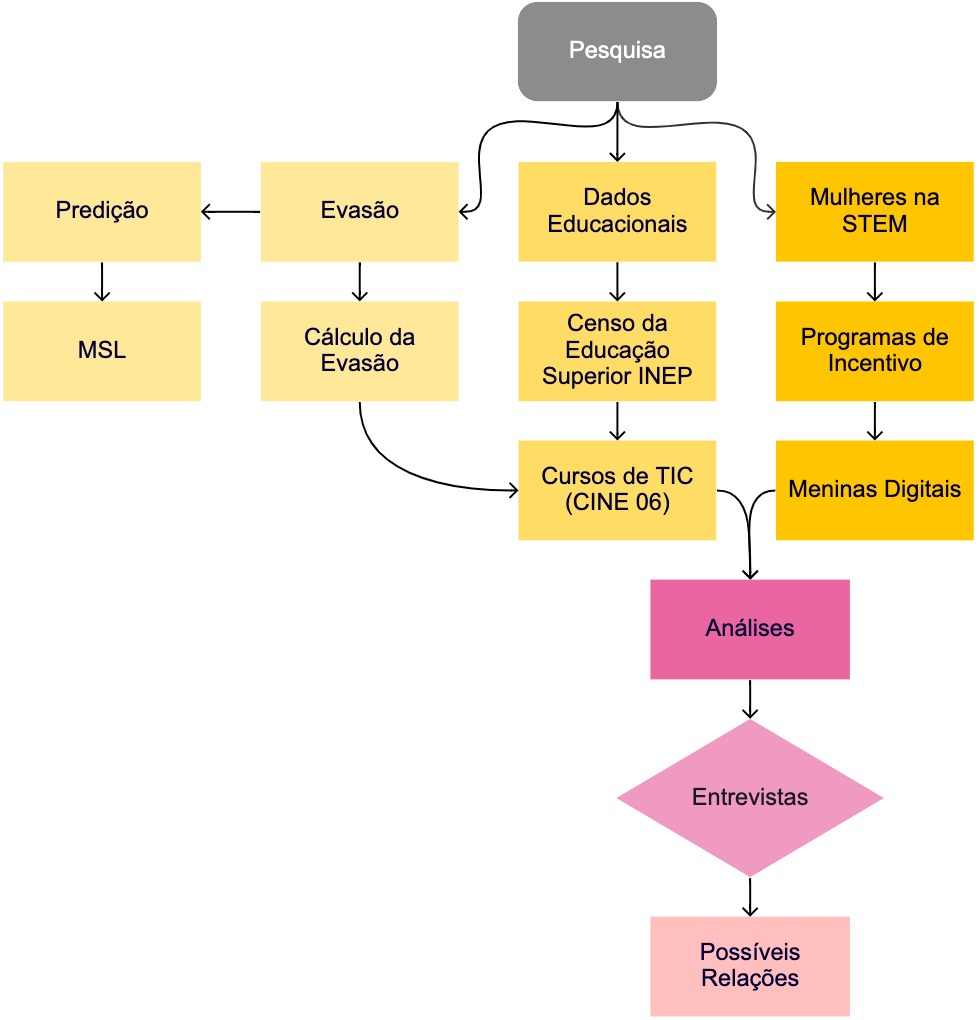
\includegraphics[width=1\textwidth]{Figuras/fluxograma.png}
\caption{Fluxograma do processo de pesquisa}
\label{fig:fluxogramaPesquisa}
\end{figure}

A Figura \ref{fig:fluxogramaPesquisa} apresenta três principais vertentes, a evasão, os dados educacionais e as mulheres na STEM. Inicialmente, a pesquisa foi em busca do estado da arte da predição da evasão, o que resultou no Mapeamento Sistemático da Literatura. 

%%%passar a limpo essa história do mapeamento e quem sabe excluir ele daqui para a defesa final, pois deixa o leitor perdido. Não sei.

Em paralelo, o estudo e exploração dos dados educacionais e do tema mulheres na STEM em busca de um objetivo e fontes de referência. Com isso, tem-se o aprofundamento em cada tema, chegando nos dados do censo da educação superior do INEP, programas de incentivo a presença e permanência de mulheres na área de STEM. Por fim, a partir de análises e entrevistas com os projetos do Programa Meninas Digitais, encontrar uma possível relação entre a presença das mulheres nos cursos de Computação e Tecnologias da Informação e Comunicação e as ações dos projetos parceiros do Programa Meninas Digitais.


\section{Mapeamento Sistemático da Literatura}\label{sec:Mapeamento}


Antes da escolha do tema da presente dissertação o ambiente da evasão foi explorado e além dos trabalhos relacionados encontrados na literatura, um Mapeamento Sistemático da Literatura (MSL) foi produzido em conjunto com o grupo de iniciação científica e está em processo de finalização para submissão. Apresenta-se aqui um panorama geral sobre o MSL.

\subsection{Processo do Mapeamento}\label{sec:procMapeamento}
O MSL realizado segue a diretriz proposta por \citeonline{petersen:2015} que apresenta as seguintes etapas: definição das questões de pesquisa, processo de busca (formulação de string de busca e realização da busca em bases acadêmicas), seleção dos estudos com base em critérios de inclusão e exclusão, análise dos estudos (extração e categorização dos dados) visando responder às questões de pesquisa.

\subsection{Objetivos e Questões de Pesquisa}\label{sec:objQuestoes}
O MSL tem o objetivo de identificar o estado da literatura sobre o estudo da predição de estudantes que possam evadir e a classificação da evasão em diferentes contextos educacionais, este trabalho definiu cinco questões de pesquisa:

\begin{itemize}
\item \textbf{Q1}: Como é definido o conceito de evasão em diferentes contextos educacionais?
\item \textbf{Q2}: Quais são as técnicas e algoritmos utilizados nos estudos sobre a predição da evasão em diferentes contextos educacionais?
\item \textbf{Q3}: Quais são os contextos educacionais em que esses estudos são realizados?
\item \textbf{Q4}: Quais elementos e características são usados como recursos nos modelos de predição?
\item \textbf{Q5}: Quais são os critérios usados para avaliar os modelos e algoritmos de predição?
\end{itemize}

\subsection{Processo de Pesquisa}
As seções a seguir detalham mais sobre como o MSL foi realizado e como os artigos foram selecionados.

\subsubsection{Formulação de string}
O primeiro passo no processo de busca é a formulação da \textit{string} de busca. Três conjuntos de palavras-chave foram escolhidos com base na área de pesquisa:

\begin{itemize}
\item \textbf{Evasão}: palavras relacionadas a evasão.
\item \textbf{Educação}: palavras que fazem referência ao contexto educacional;
\item \textbf{Predição}: palavras-chave relacionadas a predição;
\end{itemize}


Após diferentes testes de palavras chaves, sinônimos e palavras relacionadas, a \textit{string} de pesquisa foi definida como:

\begin{center}
\textit{\textit{(predict*) AND (education* OR academic OR college OR student) AND (dropout OR "drop-out" OR "drop out" OR evasion OR "at-risk" OR "at risk" OR retention OR attrition)}}
\end{center}

Ressalta-se que * é um caractere curinga usado para representar um ou mais caracteres para amplificar os resultados de pesquisa.

A \textit{string} de busca foi aplicada nas bases de dados acadêmicas, também conhecidas como Mecanismos de Buscas Acadêmicas (MBAs), em 22 de novembro de 2021, e a busca foi limitada aos termos presentes nos títulos, resumos ou palavras-chave dos artigos. Os MBAs utilizados foram ACM, El Compendex, IEEE Xplore e Scopus. Essas bases foram escolhidas por serem bases referência na área da computação.

Como resultado, 85 estudos foram obtidos na ACM, 88 estudos no IEEE e 175 estudos no Scopus, totalizando 360 estudos para a fase de seleção.

\subsubsection{Critérios de inclusão e exclusão}

O objetivo deste mapeamento sistemático foi identificar e classificar artigos que pesquisam estudantes de qualquer ambiente de educacional (formal/não formal, virtual/presencial etc) que possam ter perfil de evasão. Os critérios de inclusão foram, portanto:

\begin{itemize}
\item \textbf{CI1}: artigos disponíveis para download;
\item \textbf{CI2}: artigos em inglês ou português, sendo o português a língua nativa dos autores;
\item \textbf{CI3}: artigos primários;
\item \textbf{CI4}: artigos não duplicados;
\item \textbf{CI5}: artigos completos (apresentam metodologia e discutem seus resultados).
%\item \textbf{CI5}: artigos com experimentos ou simulações relacionados à evasão em diferentes contextos educacionais, apresentam metodologia e discutem seus resultados;
\end{itemize}

Os critérios de exclusão foram:
\begin{itemize}
\item \textbf{CE1}: artigos sem experimentação ou simulação, pois são artigos que se interessam principalmente em descrever um determinado algoritmo ou método, que não tem relação com este estudo;
\item \textbf{CE2}: artigo sem explicação dos resultados, considerando que sem os resultados da pesquisa não seria possível entender o grau de eficiência dos algoritmos utilizados.
\end{itemize}

% \subsection{Análises}

% \subsection{Resultados}




\subsection{Seleção dos Artigos}\label{sec:processoPesquisa}
%Nesta seção Todo o processo de pesquisa pode ser observado no Apêndice \ref{ap:ArtigoPredicao}, mas a seguir busca-se responder superficialmente todas as questões de pesquisa que foram analisadas sobre os 143 artigos encontrados nos Mecanismos de Buscas Acadêmicas (MBA) ACM, El Compendex, IEEE Xplore e Scopus.

%Nesta Seção busca-se responder superficialmente todas as questões de pesquisa que foram analisadas sobre os 142 artigos encontrados nos Mecanismos de Buscas Acadêmicas (MBA) ACM, IEEE Xplore e Scopus. A Tabela \ref{tab:mapeamento} mostra o número de artigos selecionados de acordo com os critérios de inclusão e exclusão.
Após aplicar os critérios de inclusão e exclusão foram analisadas sobre os 142 artigos encontrados nos Mecanismos de Buscas Acadêmicas (MBA) ACM, IEEE Xplore e Scopus. A Tabela \ref{tab:mapeamento} mostra o número de artigos selecionados de acordo com cada um desses critérios.
 
\begin{table}[H]
\centering
\caption{Total de artigos por critério de inclusão e exclusão}
\label{tab:mapeamento}
\resizebox{\columnwidth}{!}{%
\begin{tabular}{llllll}
                                                                                              & \textbf{MBA}                                 & \textbf{Scopus}          & \textbf{ACM}             & \textbf{IEEE}            & \textbf{Total}           \\ \hline
\multicolumn{1}{|l|}{}                                                                        & \multicolumn{1}{l|}{Retorno Inicial}                         & \multicolumn{1}{l|}{289} & \multicolumn{1}{l|}{118} & \multicolumn{1}{l|}{102} & \multicolumn{1}{l|}{509} \\ \hline
\multicolumn{1}{|l|}{\cellcolor[HTML]{C0C0C0}}                                                & \multicolumn{1}{l|}{Artigos disponíveis para download}       & \multicolumn{1}{l|}{277} & \multicolumn{1}{l|}{118} & \multicolumn{1}{l|}{99}  & \multicolumn{1}{l|}{494} \\ \cline{2-6} 
\multicolumn{1}{|l|}{\cellcolor[HTML]{C0C0C0}}                                                & \multicolumn{1}{l|}{Artigos em inglês ou português}          & \multicolumn{1}{l|}{269} & \multicolumn{1}{l|}{111} & \multicolumn{1}{l|}{99}  & \multicolumn{1}{l|}{479} \\ \cline{2-6} 
\multicolumn{1}{|l|}{\cellcolor[HTML]{C0C0C0}}                                                & \multicolumn{1}{l|}{Artigos primários}                       & \multicolumn{1}{l|}{265} & \multicolumn{1}{l|}{107} & \multicolumn{1}{l|}{98}  & \multicolumn{1}{l|}{470} \\ \cline{2-6} 
\multicolumn{1}{|l|}{\cellcolor[HTML]{C0C0C0}}                                                & \multicolumn{1}{l|}{Artigos não duplicados}                  & \multicolumn{1}{l|}{263} & \multicolumn{1}{l|}{100} & \multicolumn{1}{l|}{95}  & \multicolumn{1}{l|}{458} \\ \cline{2-6} 
\multicolumn{1}{|l|}{\multirow{-5}{*}{\cellcolor[HTML]{C0C0C0}\textbf{Critério de Inclusão}}} & \multicolumn{1}{l|}{Artigos completos}                       & \multicolumn{1}{l|}{263} & \multicolumn{1}{l|}{99}  & \multicolumn{1}{l|}{94}  & \multicolumn{1}{l|}{456} \\ \hline
\multicolumn{1}{|l|}{\cellcolor[HTML]{C0C0C0}}                                                & \multicolumn{1}{l|}{Artigos sem experimentação ou simulação} & \multicolumn{1}{l|}{70}  & \multicolumn{1}{l|}{62}  & \multicolumn{1}{l|}{57}  & \multicolumn{1}{l|}{160} \\ \cline{2-6} 
\multicolumn{1}{|l|}{\multirow{-2}{*}{\cellcolor[HTML]{C0C0C0}\textbf{Critério de Exclusão}}} & \multicolumn{1}{l|}{Artigos sem explicação dos resultados}   & \multicolumn{1}{l|}{62}  & \multicolumn{1}{l|}{55}  & \multicolumn{1}{l|}{54}  & \multicolumn{1}{l|}{142} \\ \hline
                                                                                              &                                                              &                          &                          & Total                    & 142                     
\end{tabular}%
}
\end{table}

Os 142 artigos selecionados são descritos na Tabela \ref{tab:mapeamentoArtigos} disposta no Apêndice \ref{ap:tabelaApendiceMSL}, onde a primeira coluna indica o número de identificação e a segunda coluna a referência completa e estão ordenados alfabeticamente pelo título do artigo.


Com os 142 artigos definidos e expostos, a subseção \ref{sub:Resultados} apresenta de forma resumida a resposta das questões de pesquisa. O processo de seleção foi realizado por um grupo de pesquisadores que contou com a mestranda deste trabalho e 4 estudantes da iniciação científica, todos apoiados por uma pesquisadora sênior. Cada artigo foi avaliado por 2 pesquisadores, os quais observaram separadamente 26 características dos artigos selecionados para depois compararem os resultados encontrados e fazerem uma discussão caso encontrassem disparidades. 

As características observadas foram: Título do artigo, autores, qual local foi publicado, ano de publicação, em qual MBA foi encontrado, qual critério de inclusão se encaixa, qual critério de exclusão, língua, país da universidade dos autores, objetivo do artigo (dividido em 8 categorias gerais), qual conceito de evasão utiliza como base, as técnicas e algoritmos utilizadas para a predição, as dimensões da base de dados, os fatores ou características observados, ensino formal ou informal, ambiente educacional, dados reais ou simulados, duração do estudo, momento da predição, o que avaliou, quais critérios utilizou, os resultados e um item para as observações.


\subsection{Resultados e Discussões}\label{sub:Resultados}

\subsubsection{Q1 - Como é definido o conceito de evasão em diferentes contextos educacionais?}\label{sub:q1}

Para buscar uma definição de evasão nos artigos analisados, fez-se uma nuvem de palavras sobre todos os conceitos adotados, resultando na Figura \ref{fig:nuvemDePalavras}

\begin{figure}[H]
\centering
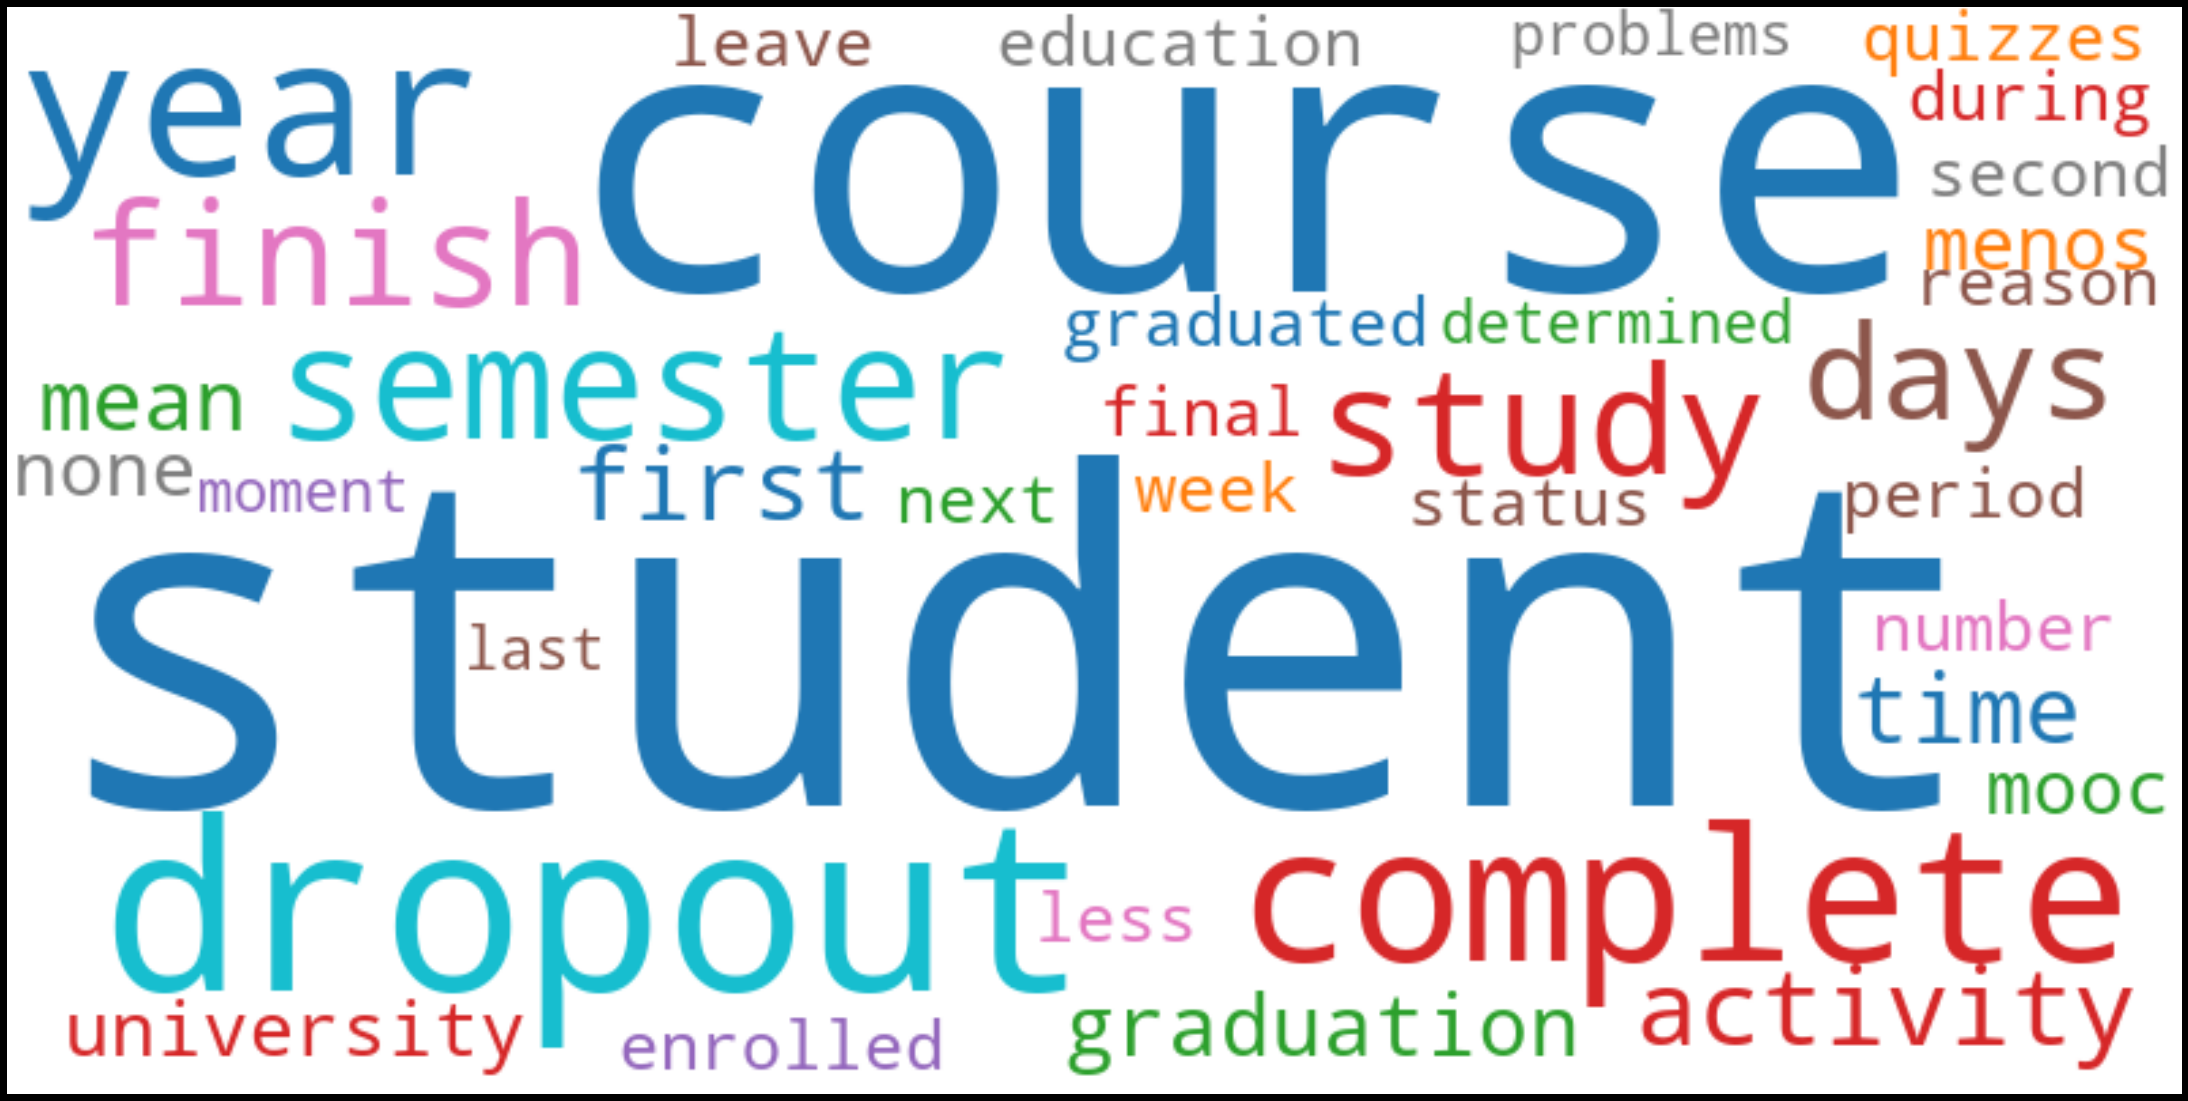
\includegraphics[width=1\textwidth]{Figuras/100_palavras_dropout.png}
\caption{Nuvem de palavras da classificação de evasão}
\label{fig:nuvemDePalavras}
\end{figure}

Observa-se na Figura \ref{fig:nuvemDePalavras} que as palavras mais frequentes nas classificações de evasão são estudante, curso, evasão, semestre, ano, completo, graduado, atividade. Entende-se com isso que no momento de classificar a evasão considera-se ano, semestre, curso com maior frequência que média, problema e quiz, desta forma quando os autores observam a evasão foi mais comum o período/tempo do que rendimento do estudante.

As abordagens mais presentes para a classificação de evasão foram a de abandono do estudo independente do motivo (artigos com ID 22, 23, 48, 70 e 84) e a de estudantes que não completaram o curso em um determinado período de tempo (artigos com ID 1, 6, 25, 37, 49, 57, 78, 83, 85, 88, 100, 115 e 116). No caso de cursos online, estudantes que não interagem com a plataforma por um determinado período de tempo (artigos com ID 4, 19, 26, 31, 42, 75 e 78) também são considerados evadidos.

\subsubsection{Q2 - Quais são as técnicas e algoritmos utilizados nos estudos sobre a predição da evasão em diferentes contextos educacionais?}\label{sub:q2}

Das técnicas, \textit{machine learning} foi de longe a mais utilizada, assumindo 51,4\% sobre todas as outras técnicas citadas. Logo em seguida, as técnicas mistas assumem 21,1\% e técnicas de estatística 10,5\%. As técnicas mistas apresentadas são a utilização de duas ou mais técnicas na mesma abordagem. Quanto aos algoritmos, apresenta-se na Figura \ref{fig:algoritmos} gráfico de barras com os algoritmos mais citados, com destaque para \textit{suport vector machine, decision tree} e \textit{random forest}.


\begin{figure}[H]
\centering
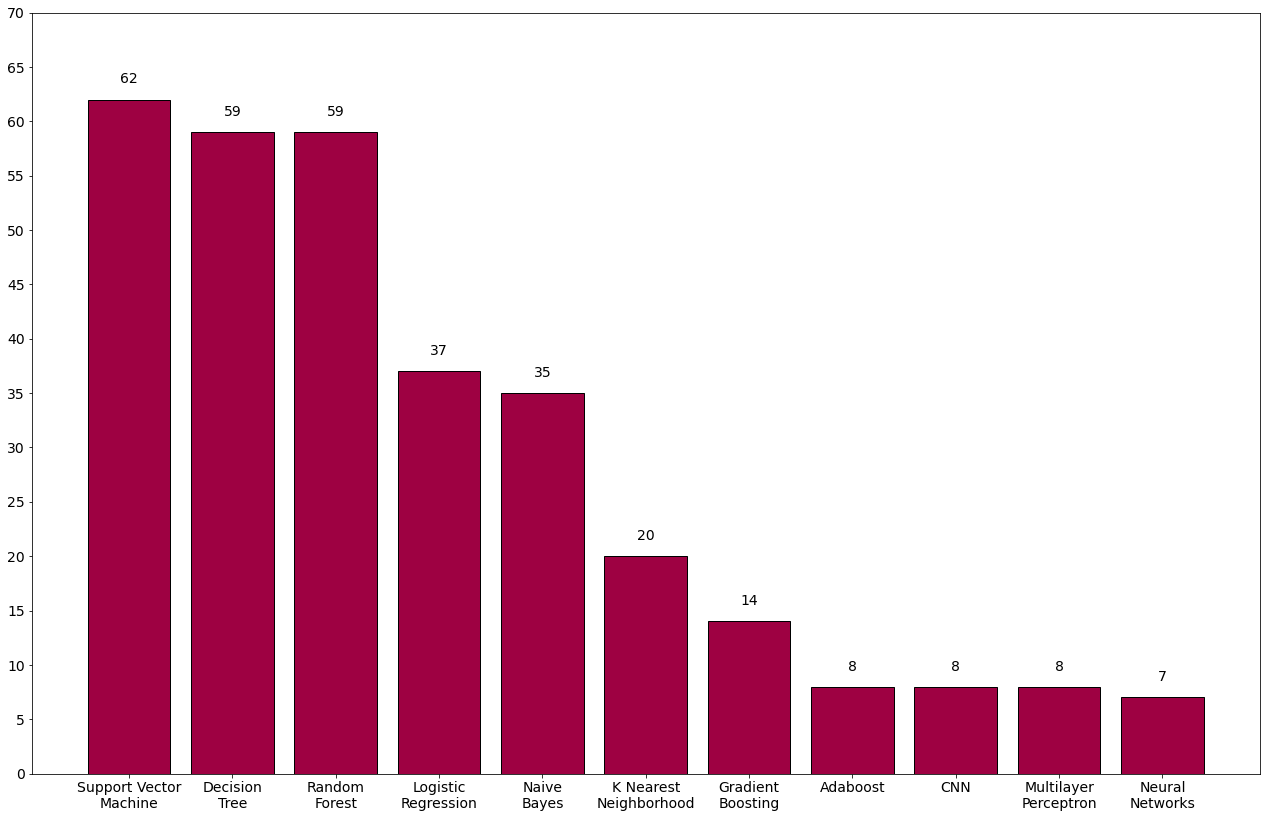
\includegraphics[width=1\textwidth]{Figuras/algoritmos_utilizados.png}
\caption{Algoritmos utilizados para predição da evasão}
\label{fig:algoritmos}
\end{figure}


\subsubsection{Q3 - Quais são os contextos educacionais em que esses estudos são realizados?}\label{sub:q3}

Para responder a questão 3 traz-se a Figura \ref{fig:contexto_ano} que mostra ano a ano o número de artigos por cada contexto educacional abordado. Os conceitos educacionais são classificados como artigos que observaram dados relacionados a certificações, cursos, ensino médio, graduação, mestrado e doutorado.

Na Figura \ref{fig:contexto_ano} dois contextos estão em uma crescente, o contexto de graduação, que também mostra-se predominante e o contexto de cursos.

\begin{figure}[H]
\centering
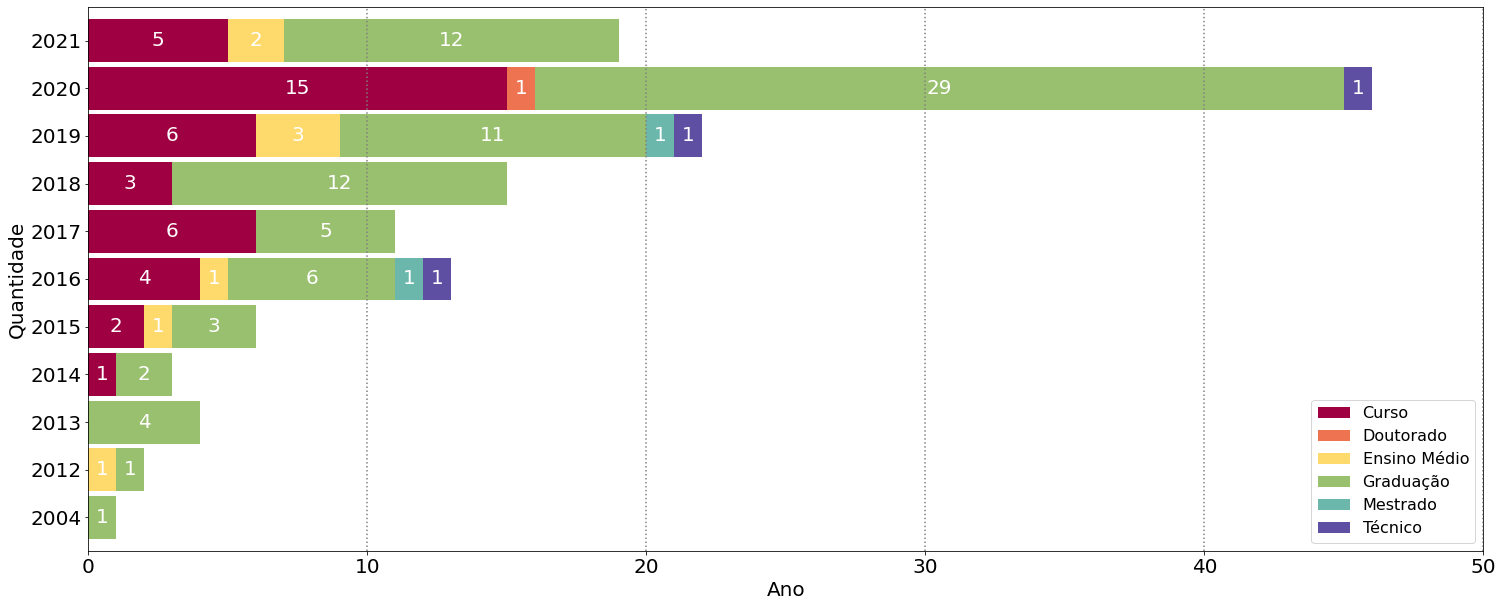
\includegraphics[width=1\textwidth]{Figuras/contexto_ano.png}
\caption{Distribuição de artigos por ano de publicação e contexto}
\label{fig:contexto_ano}
\end{figure}

\subsubsection{Q4 - Quais elementos e características são usados como recursos nos modelos de predição?}\label{sub:q4}

A nuvem de palavra da Figura \ref{fig:nuvemElementosCaracteristicas} mostra quais foram os principais elementos e características utilizadas para aplicar nos modelos de predição.

\begin{figure}[H]
\centering
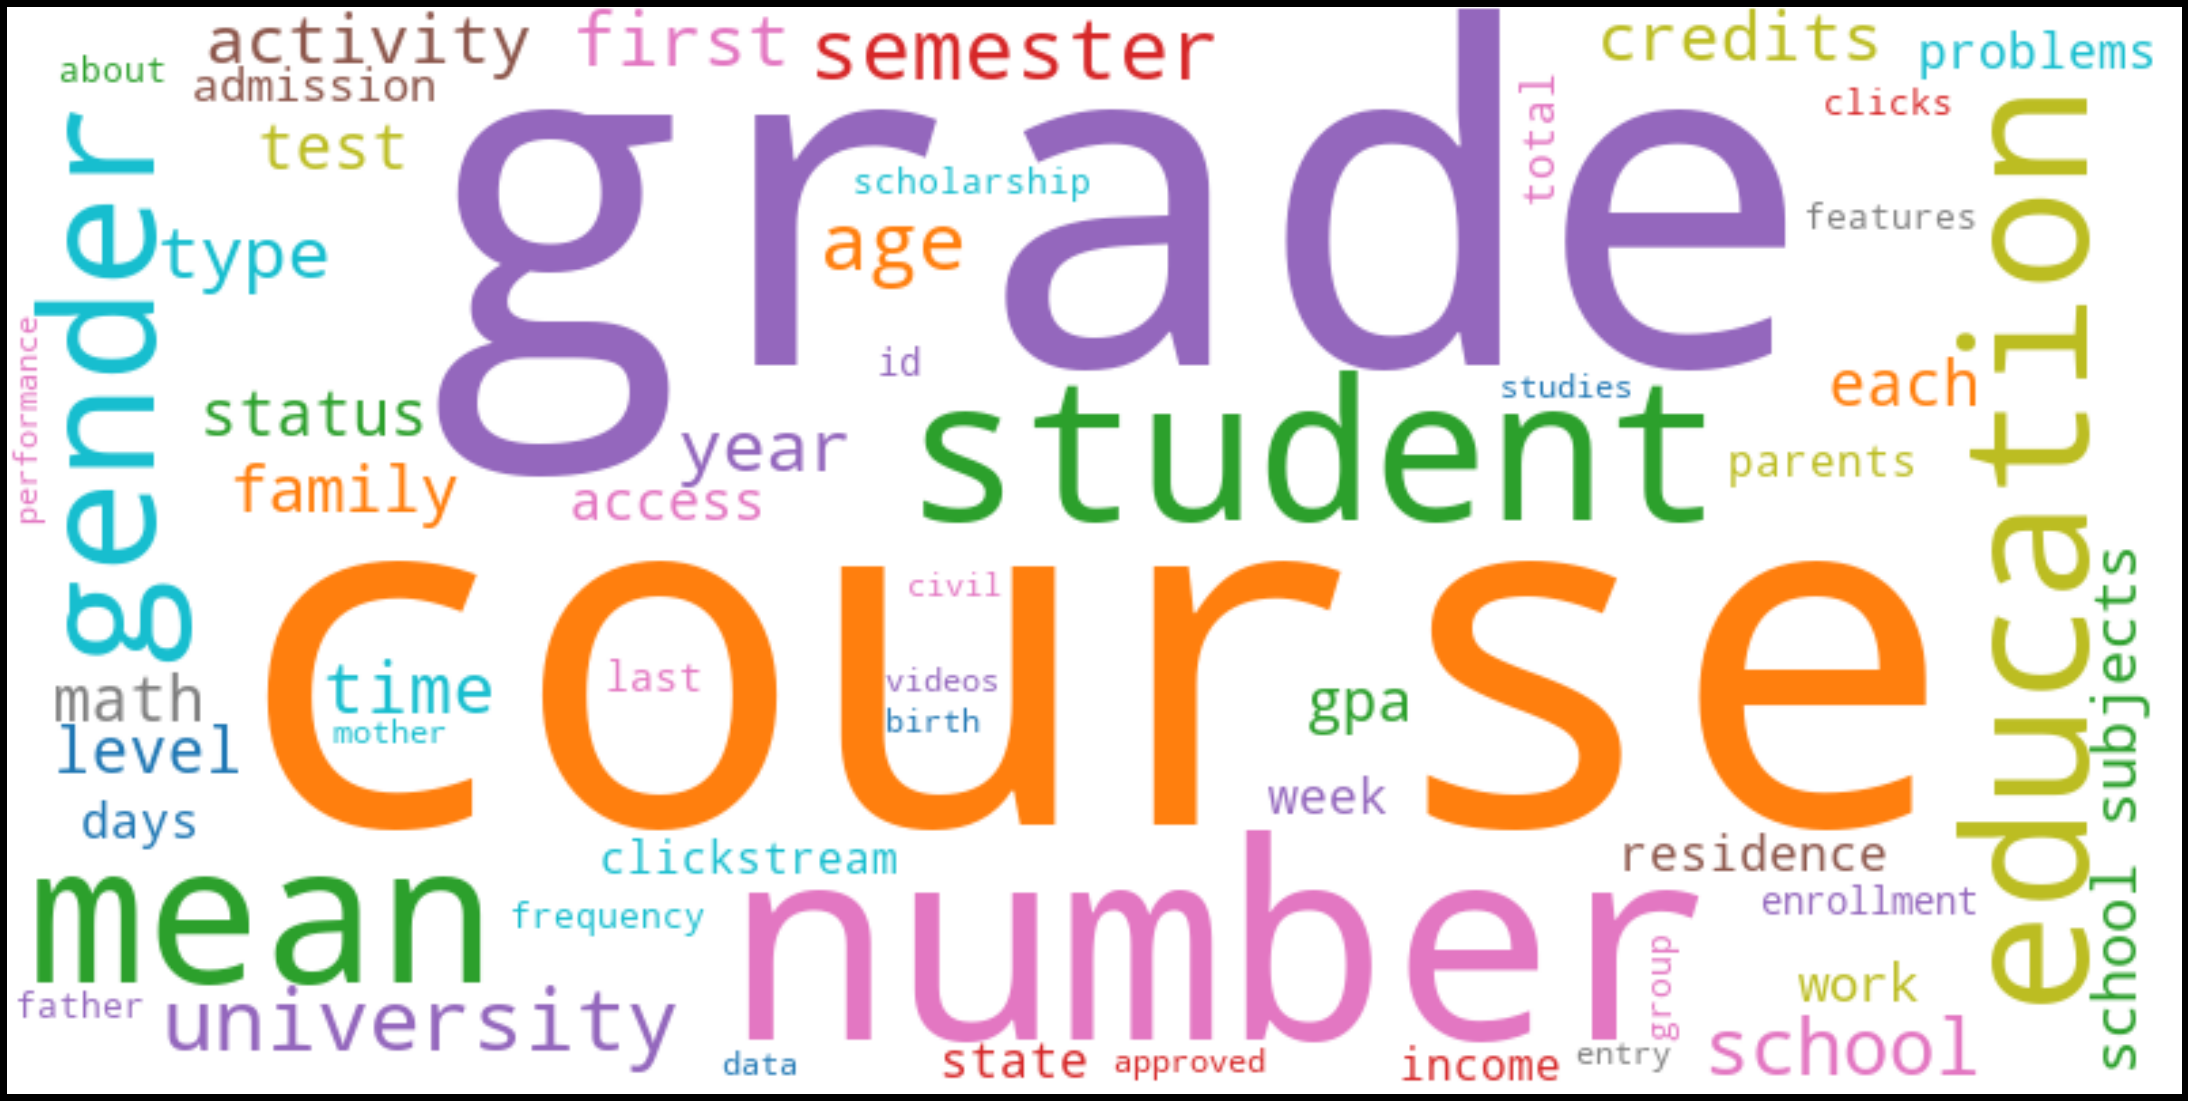
\includegraphics[width=1\textwidth]{Figuras/100_palavras_features.png}
\caption{Nuvem de palavras dos elementos e características usados nos modelos de predição}
\label{fig:nuvemElementosCaracteristicas}
\end{figure}

A nuvem da Figura \ref{fig:nuvemElementosCaracteristicas} mostra que curso é muito considerado e grade também, que do inglês pode significar grade curricular, grau, curso ou até nota, o que faz sentido, pois a maioria dos fatores esta de alguma forma ligada ao curso. 

É interessante observar que média e gênero aparecem basicamente com a mesma frequência, trazendo a importância do gênero na predição da evasão.

Número refere-se a uma série de características, sendo algumas delas: número de semestres cursados antes da evasão, número de créditos, número de disciplinas obrigatórias por semestre, número de novos alunos, número de alunos que evadiram, número de alunos que continuam no curso, número de alunos que se formam, e outros, que foram valores importantes para alguns dos modelos de predição.“Renda”, “bolsa” e “família” referem-se às necessidades, carências financeiras e a aquisição de bolsas mostram influência na evasão dos estudantes. 

Observa-se também fatores relacionados a ensino remoto, “Acesso”, “cliques” e “vídeos”estão associados a quanta interação há entre os estudantes e as mídias digitais ou online disponibilizadas em seus cursos. 

\subsubsection{Q5 - Quais são os critérios usados para avaliar os modelos e algoritmos de predição?}\label{sub:q5}

O critério de avaliação para os modelos e algoritmos que apareceu em maior frequência foi a acurácia, muito possivelmente por conta do que mostrou a Figura \ref{fig:algoritmos}, onde quase todos os modelos são avaliados por meio da acurácia. Logo em seguida vem o critério da precisão como forma de avaliar os modelos de algoritmos de predição. 

Além disso a acurácia é possivelmente a métrica mais simples, onde é calculada com o número de acertos (positivos) divido pelo número total de exemplos.

Observa-se ainda que a maioria dos trabalhos utilizam-se de mais de um critério de avaliação, unindo por exemplo Acurácia, Valor Presente Líquido, Precisão e Revocação na mesma avaliação de algoritmo. 

\subsection{Limitações e Ameaças a validade}\label{sub:limitacoeseameacas}
Para a garantia da qualidade de pesquisa é necessário levantar as limitações e ameaças a sua validade a fim de orientar a reprodutibilidade da pesquisa.

\subsubsection{Viés do Pesquisador}

A pesquisa foi planejada e realizada pelo mesmo grupo de pesquisa, desta forma tudo o que foi produzido pode ter sofrido um direcionamento. Para amenizar este quesito, todos os estudos dos artigos, as análises e respostas as questões de pesquisa foram feitas por pares de pesquisadores. A dupla realizou separadamente seu trabalho e depois fizeram reuniões de consenso. Após os resultados foram discutidos com todo o grupo, inclusive a pesquisadora sênior.

\subsubsection{Viés de amostragem}

A amostra selecionada pode estar nichada a um determinado local não apresentando a população completa, sendo uma ameaça aos resultados do mapeamento. Para a redução deste risco, primeiramente optou-se por mecanismos amplamente utilizados na área de computação e foi feita uma busca com a mesma \textit{string} e no mesmo período

\subsection{Considerações do MSL}
%explicando o tema
Durante a elaboração e análises do MSL, os autores perceberam que um passo atrás era necessário, desta forma nasceram as novas questões relacionadas ao tema desta dissertação, onde não se observa mais os algoritmos de predição da evasão e sim os conceitos e relações a partir do tema evasão. Por isso, a presente Seção apresentou um compilado resumido do que é o mapeamento.

Algumas questões do MSL podem ser tiradas como aprendizado para a atual pesquisa, por exemplo a Questão 1, que busca saber as definições de evasão. Observa-se a importância do gênero para os elementos e características nas variáveis utilizadas nos modelos de predição.
No demais, o MSL mostra-se promissor para sua finalização e possível publicação.


%%%Como resposta desta questão surge a Figura \ref{fig:nuvemDePalavras}, uma nuvem de palavras com estas definições, que podem ser melhor entendidas com a leitura completa do Apêndice \ref{ap:ArtigoPredicao}.

% Para maior completude do estudo, foi realizado um Mapeamento Sistemático da Literatura (MSL). MSLs são definidos como estudos secundários cujo objetivo é fornecer uma visão geral de uma área específica com base em estudos primários e na análise quantitativa das contribuições desses estudos. O principal objetivo de um estudo de mapeamento é fornecer uma visão geral de uma área de pesquisa e classificar a quantidade, forma de pesquisa e possíveis descobertas. Para observar padrões, é comum traçar a frequência de publicação ao longo do tempo \shortcite{petersen:2015}. O presente MSL buscou responder questões mais gerais sobre o tema da evasão.

% \section{Processo de mapeamento}

% O mapeamento sistemático realizado segue a diretriz proposta por \citeA{petersen:2015} que apresenta as seguintes etapas: definição das questões de pesquisa, processo de busca (formulação de strings de busca e realização da busca em bases acadêmicas), seleção dos estudos com base em critérios de inclusão e exclusão, análise dos estudos (extração e categorização dos dados) visando responder às questões de pesquisa. Cada uma dessas etapas é descrita nas próximas subseções.

% \subsection{Questões de Pesquisa}
% Com o objetivo de identificar o estado da literatura sobre o estudo da evasão em diferentes contextos educacionais e a predição de estudantes que possam evadir, este trabalho definiu cinco questões de pesquisa:

% \begin{itemize}
% \item \textbf{Q1}: Como é definido o conceito de evasão em diferentes contextos educacionais?
% \item \textbf{Q2}: Quais são as técnicas e algoritmos utilizados nos estudos sobre a previsão da evasão em diferentes contextos educacionais?
% \item \textbf{Q2}: Quais são os contextos educacionais em que esses estudos são realizados?
% \item \textbf{Q4}: Quais elementos e características são usados como recursos nos modelos de previsão?
% \item \textbf{Q5}: Quais são os critérios usados para avaliar os modelos e algoritmos de previsão?
% \end{itemize}





\section{Entendimento e preparação das bases utilizadas}\label{sec:EntendimentoDados}

Os dados analisados vão até o ano de 2019 pois durante a etapa das análises era o ano mais recende disponível pelo INEP. Além disso, para uma possível atualização, tendo em vista que o censo da educação superior de 2020 foi publicado em março de 2022, seria necessário adaptação e novo entendimento da base, pois novamente o padrão de organização foi alterado, inviabilizando também a forma com que a evasão é calculada na presente dissertação.

Os dados do INEP no momento em que foram baixados estavam disponíveis como apresentados nesta dissertação, porém foram parcialmente retirados do ar no dia 21 de fevereiro de 2022. Para o acesso dos dados mais recentes (referentes ao ano de 2020), o Serviço de Acesso a Dados Protegidos (Sedap) do Governo Federal Brasileiro permite de forma controlada e restrita o acesso às bases, por meio de um conjunto de protocolos, onde os pesquisadores e a sociedade em geral podem ter o acesso às bases de dados relacionadas aos Censos e Avaliações produzidas pela autarquia, exclusivamente para fins de pesquisa e de estudo.

Para analisar a presença das mulheres nos cursos de Computação e Tecnologias da Informação e Comunicação, é necessário observar o contexto dos dados. A presença e permanência das mulheres nesta área pode ser analisada a partir de seu inverso, a evasão e para o início das análises foi preciso dedicar tempo para o entendimento dos dados. Foram três fontes principais de dados, INEP, e-MEC e dados do CINE Brasil. 

Os dados do INEP a partir de 2009 até 2019 totalizam 10 anos de histórico de estudantes, professores e IES. As bases de dados do INEP utilizadas de cada ano são divididas em 6 partes, onde estão guardados os dados gerais do censo, os dados da IES, dos docentes, estudantes, locais e uma tabela auxiliar do CINE. Das 6 partes, as tabelas maiores e mais complexas são as tabelas de estudante e docente, juntas possuem mais de 170 colunas. Como um auxílio o INEP disponibiliza um dicionário de variáveis, para entendimento do que cada coluna significa. No caso dos dados dos estudantes o dicionário de variáveis traz informações das 105 variáveis disponíveis sobre os estudante, algumas delas são:

\begin{itemize}
    \item CO\_CURSO - Código único de identificação do curso gerado pelo E-MEC;
    \item CO\_CINE\_ROTULO - Código de identificação do curso, conforme adaptação da Classificação Internacional Normalizada da Educação Cine/Unesco;
    \item ID\_ALUNO - Código de identificação gerado pelo Inep para o aluno da educação superior;
    \item TP\_COR\_RACA - Tipo da cor/raça do aluno;
    \item TP\_SEXO - Informa o sexo do aluno;
    \item NU\_IDADE - Idade que o aluno completa no ano de referência do Censo;
    \item IN\_DEFICIENCIA - Informa se o aluno é uma pessoa com deficiência, transtorno global do desenvolvimento ou altas habilidades/superdotação;
    \item IN\_INGRESSO\_VESTIBULAR - Informa se o aluno ingressou no curso por vestibular;
    \item IN\_INGRESSO\_ENEM - Informa se o aluno ingressou no curso pelo Enem;
    \item IN\_INGRESSO\_OUTRO\_TIPO\_SELECAO - Informa se o aluno ingressou no curso por outros tipos de seleção;
    \item IN\_ATIVIDADE\_EXTRACURRICULAR - Informa se o aluno participa de algum tipo de atividade extracurricular (estágio não obrigatório, extensão, monitoria e pesquisa).
\end{itemize}

Com a discriminação parcial desta base, é possível observar que ela se correlaciona com as outras duas bases, tanto a do e-MEC na variável CO\_CURSO, quanto a do CINE na variável CO\_CINE\_ROTULO.

As classificações CINE são disponibilizadas pelo INEP em uma tabela auxiliar intitulada TB\_AUX\_CINE\_BRASIL. Para mais detalhes a Diretoria de Estatísticas Edicionais (DEED) disponibiliza o Manual para Classificação dos Cursos de Graduação e Sequenciais que apresenta a estrutura CINE Brasil e todos os procedimentos para classificá-los, tendo como objetivo orientar as IES a realizarem a classificação adequada de seus cursos \cite{CINE}. Com esta classificação, busca-se então os cursos classificados como 06 Computação e Tecnologias da Informação e Comunicação (TIC) pelo CINE.

Já os dados disponíveis pelo e-MEC podem ser pesquisados manualmente onde o usuário tem a opção de fazer uma busca por IES, curso de graduação ou curso de especialização. Escolhendo a busca por curso de graduação é possível buscar a partir do nome do curso, unidade federal, município, gratuidade do curso, modalidade (presencial ou a distância) e grau (bacharelado, licenciatura, tecnólogo ou sequencial).

Como a base do INEP apresenta apenas os códigos de IES e cursos, para levantamento de todos os cursos com seus respectivos nomes é necessário cruzar as informações com a base do e-MEC. Após executar uma busca na base do e-MEC o retorno apresenta-se em formato CSV contendo 56 variáveis, dente elas Código da IES, Sigla da IES, Nome da IES, Código do Curso, Nome do Curso e Código CINE tornando possível conferir e cruzar os dados provindos do INEP e do e-MEC.


O foco nessa dissertação são cursos classificados como 06 Computação e Tecnologias da Informação e Comunicação (TIC) presentes nos dados do INEP dos anos de 2009 a 2019 que estejam relacionados com algum projeto do programa Meninas Digitais.



%--Sabendo disso, o presente trabalho analisa os cursos classificados como 06 Computação e Tecnologias da Informação e Comunicação (TIC).

%A base de dados disponibilizada pelo INEP já sofreu algumas alterações quanto o padrão organizacional, desta forma o presente trabalho utiliza-se dos anos mais próximos desta publicação em que o padrão de dados foi o mesmo, de 2009 a 2019.

%\section{Preparação dos Dados}\label{sec:PreparacaoDados}
%Outro problema de inconsistência de dados foi encontrado no relacionamento entre as bases do INEP e do e-MEC --TABELA COM OS PROJETOS E CÓDIGOS DE CURSOS QUE NAO TEM NA BASE INEP MAS TEM NO EMEC--

Como as bases utilizadas são muito extensas e cheias de informações tornam as analises sobre tais dados ainda mais complexas, cada ano possui em média 2GB. Apesar disso não é necessário o uso completo de todas as informações para cada análise presente na dissertação. Desta forma fez-se uma limpeza inicial, excluindo algumas variáveis para tornar o processo mais rápido e de fácil execução. Outra abordagem utilizada para facilitar o uso das informações é a criação de bases menores, com apenas colunas específicas que estarão em uso para as análises.



\section{Projetos Parceiros do Programa Meninas Digitais}\label{sec:ProjetosLevantados}
Após o levantamento dos dados para as análises da presença, evasão e permanência das mulheres na área de Computação e Tecnologias da Informação e Comunicação, inicia-se a busca pelos projetos do programa Meninas Digitais, que foi o programa escolhido para a presente pesquisa por ser um programa referência no Brasil e na América Latina em equidade de gênero nas carreiras de Tecnologia da Informação e Comunicação.

O programa Meninas Digitais tem como principal objetivo a divulgação da área de computação e suas tecnologias para despertar o interesse de meninas e mulheres. Foi criado no ano de 2011 sob a coordenação da Secretaria Regional da SBC em Mato Grosso e, em 2015, foi institucionalizado pela SBC, recebendo sua chancela, como programa de interesse nacional da comunidade de Computação \cite{meninas:digitais}. O programa surgiu de uma discussão no \textit{Women in Information Technology} (WIT), evento base do Congresso da Sociedade Brasileira de Computação (CSBC) \cite{meninas:digitais}.

Para que a ideia tomasse forma, o Programa conta com a colaboração de multiplicadores de proposta, os Projetos Parceiros (\textit{sister projects}) presentes nas instituições para disseminar a ideia no território nacional.

Todo o processo de mapeamento dos projetos do programa Meninas Digitais ocorreu no dia 2 de abril de 2022 a partir de seu site\footnote{https://meninas.sbc.org.br/projetos/} particular. Organizados na Tabela \ref{tab:ProjetosMeninasDigitais} todas as informações foram retiradas exclusivamente deste site. As informações disponíveis por projetos são nome do projeto, status (projeto ativo ou concluído), ano, contato e endereço, mas nem sempre todas as informações estavam presentes, sua última atualização informada é do dia 13 de junho de 2020.




%%============TABELA===================

\begin{longtable}{|l|l|l|}
\caption{Projetos do Programa Meninas Digitais}
\label{tab:ProjetosMeninasDigitaisD}\\
\hline
\rowcolor[HTML]{C0C0C0} 
\textbf{Nome do Projeto}                                                                                                                                    & \textbf{Status}              & \textbf{Início}                \\ \hline
\endfirsthead
%
\multicolumn{3}{c}%
{{\bfseries Tabela \thetable\ continuação da página anterior}} \\
\hline
\rowcolor[HTML]{C0C0C0} 
\textbf{Nome do Projeto}                                                                                                                                    & \textbf{Status}              & \textbf{Início}                \\ \hline
\endhead
%
  
{\color[HTML]{000000} \#include \textless GURIAS \textgreater{}}                                                                                            & {\color[HTML]{000000} Ativo} & {\color[HTML]{000000} 2018} \\ \hline
  
\#include \textless meninas.uff \textgreater{}                                                                                                              & Ativo                        & 2016                        \\ \hline
  
\#include \textless{}girls\textgreater{}                                                                                                                    & Ativo                        & 2021                        \\ \hline
ADA Code – Meninas Digitais Rondônia                                                                                                                        & Concluído                    & 2017                        \\ \hline
ADAs                                                                                                                                                        & Ativo                        & 2017                        \\ \hline
  
ALICE                                                                                                                                                       & Ativo                        & 2019                        \\ \hline
AmbientAda                                                                                                                                                  & Ativo                        & 2017                        \\ \hline
Android Smart Girls                                                                                                                                         & Concluído                    & 2014-2015                   \\ \hline
  
Aprenda a Programar Jogando                                                                                                                                 & Ativo                        & 2016                        \\ \hline
  
B-Lab Girls                                                                                                                                                 & Ativo                        & 2018                        \\ \hline
Binary Girls                                                                                                                                                & Ativo                        & 2017                        \\ \hline
  
BitGirls                                                                                                                                                    & Ativo                        & 2018                        \\ \hline
  
BitRosa – Elas na Computação                                                                                                                                & Ativo                        & 2015                        \\ \hline
Bits de Ada                                                                                                                                                 & Ativo                        & 2016                        \\ \hline
  
Byte’s Girls                                                                                                                                                & Ativo                        & 2019                        \\ \hline
  
Caliandras Digitais                                                                                                                                         & Ativo                        & 2020                        \\ \hline
  
Catarinas                                                                                                                                                   & Ativo                        & 2016                        \\ \hline
CHICA BYTES                                                                                                                                                 & Ativo                        & 2019                        \\ \hline
  
Cintia (Ciência e Tecnologia da Informação com Elas)                                                                                                        & Ativo                        & 2018                        \\ \hline
Code and Ladies                                                                                                                                             & Ativo                        & 2019                        \\ \hline
Code Queens                                                                                                                                                 & Ativo                        & 2020                        \\ \hline
Code Rosa                                                                                                                                                   & Ativo                        & 2016                        \\ \hline
  
Coletivo Min@                                                                                                                                               & Ativo                        & 2018                        \\ \hline
Compsi Girls                                                                                                                                                & Ativo                        & 2019                        \\ \hline
Computer Girls                                                                                                                                              & Ativo                        & 2016                        \\ \hline
  
Conectadas                                                                                                                                                  & Ativo                        & 2017                        \\ \hline
  
Corte de Lovelace                                                                                                                                           & Ativo                        & 2017                        \\ \hline
CTRL + Gurias                                                                                                                                               & Ativo                        & 2017                        \\ \hline
  
Cunhantã Digital                                                                                                                                            & Ativo                        & 2015                        \\ \hline
Cunharandu Bots                                                                                                                                             & Concluído                    & 2013-2015                   \\ \hline
  
\begin{tabular}[c]{@{}l@{}}DAMA – Disseminação e Apoio à participação de \\ Mulheres na Área de Computação\end{tabular}                                     & Ativo                        & 2020                        \\ \hline
\begin{tabular}[c]{@{}l@{}}Desenvolvimento do Raciocínio Lógico no \\ Ensino Fundamental e Médio\end{tabular}                                               & Ativo                        & 2013                        \\ \hline
  
Developer Girls                                                                                                                                             & Ativo                        & 2017                        \\ \hline
Digital Girls In Rio                                                                                                                                        & Concluído                    & 2016-2018                   \\ \hline
  
Divas                                                                                                                                                       & Ativo                        & 2015                        \\ \hline
  
Ei Mana!                                                                                                                                                    & Ativo                        & 2018                        \\ \hline
  
Elas Digitais IFSC                                                                                                                                          & Ativo                        & 2019                        \\ \hline
  
Elas++ (elas mais mais)                                                                                                                                     & Ativo                        & 2020                        \\ \hline
  
Emíli@s – Armação em Bits                                                                                                                                   & Ativo                        & 2013                        \\ \hline
Encoding Women                                                                                                                                              & Concluído                    & 2016-2017                   \\ \hline
Entre Adas e Marias                                                                                                                                         & Concluído                    & 2017-2017                   \\ \hline
Fatecanas                                                                                                                                                   & Ativo                        & 2019                        \\ \hline
  
FaTech Girls                                                                                                                                                & Ativo                        & 2017                        \\ \hline
FlorADAs                                                                                                                                                    & Ativo                        & 2021                        \\ \hline
  
ForGirls                                                                                                                                                    & Ativo                        & 2019                        \\ \hline
  
Garotas Applicadas                                                                                                                                          & Ativo                        & 2019                        \\ \hline
  
Garotas Tech dos Sertões de Crateús                                                                                                                         & Ativo                        & 2019                        \\ \hline
  
GECET: Garotas nas Engenharias, Ciências Exatas e Tecnologias                                                                                               & Ativo                        & 2020                        \\ \hline
  
GIRLS POWER IN PROGRAMMING                                                                                                                                  & Ativo                        & 2019                        \\ \hline
Girls’n Code                                                                                                                                                & Ativo                        & 2019                        \\ \hline
GRACE – Garotas na Computação e Empreendedorismo                                                                                                            & Ativo                        & 2017                        \\ \hline
  
GRACE – Grupo de Alunas nas Ciências Exatas                                                                                                                 & Ativo                        & 2018                        \\ \hline
Gurias Digitais                                                                                                                                             & Ativo                        & 2018                        \\ \hline
  
Gurias na Computação                                                                                                                                        & Ativo                        & 2016                        \\ \hline
IF(meninas)\{nas exatas\}                                                                                                                                   & Ativo                        & 2017                        \\ \hline
In4Girls                                                                                                                                                    & Ativo                        & 2019                        \\ \hline
Inclusão Feminina em Carreiras Tecnológicas da UFRN                                                                                                         & Ativo                        & 2020                        \\ \hline
InfoGirl (Evento)                                                                                                                                           & Ativo                        & 2014                        \\ \hline
Inova Kids Prudente                                                                                                                                         & Ativo                        & 2018                        \\ \hline
IT Girls – Garotas na Tecnologia da Informação                                                                                                              & Ativo                        & 2016                        \\ \hline
JoinGirls                                                                                                                                                   & Ativo                        & 2018                        \\ \hline
  
JUMI - Juventudes de Mujeres en Ciencia e Ingeniería                                                                                                        & Ativo                        & 2021                        \\ \hline
  
\begin{tabular}[c]{@{}l@{}}Katie: saindo do buraco negro e impulsionando as \\ meninas na computação\end{tabular}                                           & Ativo                        & 2019                        \\ \hline
KeyTech                                                                                                                                                     & Ativo                        & 2018                        \\ \hline
Link com Elas                                                                                                                                               & Ativo                        & 2019                        \\ \hline
  
Maia – Meninas Aprendendo Inteligência Artificial                                                                                                           & Ativo                        & 2018                        \\ \hline
Manas Digitais                                                                                                                                              & Ativo                        & 2018                        \\ \hline
MannaTeam                                                                                                                                                   & Ativo                        & 2016                        \\ \hline
Maria Bonita nas Ciências                                                                                                                                   & Ativo                        & 2019                        \\ \hline
MariaBIT                                                                                                                                                    & Concluído                    & 2015-2017                   \\ \hline
  
Meninas Cientistas                                                                                                                                          & Ativo                        & 2018                        \\ \hline
Meninas da ECITI                                                                                                                                            & Ativo                        & 2018                        \\ \hline
  
Meninas da Geotecnologia                                                                                                                                    & Ativo                        & 2019                        \\ \hline
Meninas Digitais Arretadas                                                                                                                                  & Ativo                        & 2016                        \\ \hline
Meninas Digitais Cáceres Pantanal Digital                                                                                                                   & Ativo                        & 2017                        \\ \hline
  
Meninas Digitais de Rio Pomba                                                                                                                               & Ativo                        & 2019                        \\ \hline
Meninas Digitais do DF                                                                                                                                      & Ativo                        & 2019                        \\ \hline
  
Meninas Digitais do Sudoeste da Bahia                                                                                                                       & Ativo                        & 2019                        \\ \hline
Meninas Digitais do Vale                                                                                                                                    & Ativo                        & 2018                        \\ \hline
  
Meninas Digitais Dourados – Heroínas Digitais                                                                                                               & Ativo                        & 2018                        \\ \hline
\begin{tabular}[c]{@{}l@{}}Meninas Digitais Empreendedoras: Inserção de mulheres \\ na área de Tecnologia da Computação e seus empreendimentos\end{tabular} & Ativo                        & 2019                        \\ \hline
Meninas Digitais IFMT Campo Novo do Parecis                                                                                                                 & Ativo                        & 2017                        \\ \hline
  
Meninas Digitais IFMT Cuiabá                                                                                                                                & Ativo                        & 2015                        \\ \hline
Meninas Digitais IFMT Tangará da Serra                                                                                                                      & Concluído                    & 2015-2017                   \\ \hline
Meninas Digitais IFSULDEMINAS                                                                                                                               & Ativo                        & 2019                        \\ \hline
  
Meninas Digitais na Baixada Fluminense                                                                                                                      & Ativo                        & 2019                        \\ \hline
  
Meninas Digitais na Computação – UNIJU                                                                                                                      & Ativo                        & 2019                        \\ \hline
  
Meninas Digitais na IENH                                                                                                                                    & Ativo                        & 2019                        \\ \hline
  
Meninas Digitais no Cerrado                                                                                                                                 & Ativo                        & 2016                        \\ \hline
Meninas Digitais Piauí                                                                                                                                      & Ativo                        & 2019                        \\ \hline
  
Meninas Digitais Regional Bahia                                                                                                                             & Ativo                        & 2016                        \\ \hline
  
Meninas Digitais Regional Mato Grosso                                                                                                                       & Ativo                        & 2015                        \\ \hline
  
Meninas Digitais Regional Sergipe                                                                                                                           & Ativo                        & 2018                        \\ \hline
  
Meninas Digitais Regional Sul                                                                                                                               & Ativo                        & 2012                        \\ \hline
  
Meninas Digitais Tchê Missões                                                                                                                               & Ativo                        & 2016                        \\ \hline
Meninas Digitais UFBA                                                                                                                                       & Ativo                        & 2016                        \\ \hline
Meninas Digitais UFMT Cuiabá                                                                                                                                & Ativo                        & 2015                        \\ \hline
  
Meninas Digitais UFSC                                                                                                                                       & Ativo                        & 2013                        \\ \hline
  
Meninas Digitais Vale do Itajaí                                                                                                                             & Ativo                        & 2018                        \\ \hline
  
Meninas High Tech                                                                                                                                           & Ativo                        & 2019                        \\ \hline
Meninas Mais Mais                                                                                                                                           & Ativo                        & 2014                        \\ \hline
Meninas na Ciência da Computação                                                                                                                            & Ativo                        & 2014                        \\ \hline
Meninas na Computação                                                                                                                                       & Ativo                        & 2014                        \\ \hline
Meninas na Computação para Escolas Públicas                                                                                                                 & Ativo                        & 2019                        \\ \hline
Meninas na Computação UNIFAP                                                                                                                                & Ativo                        & 2018                        \\ \hline
  
Meninas Paid’éguas                                                                                                                                          & Ativo                        & 2019                        \\ \hline
  
Meninas Programadoras                                                                                                                                       & Ativo                        & 2021                        \\ \hline
Meninas Também Jogam                                                                                                                                        & Ativo                        & 2015                        \\ \hline
Meninas Tecnológicas                                                                                                                                        & Ativo                        & 2018                        \\ \hline
  
Meninas.comp – Computação Também é Coisa de Menina!                                                                                                         & Ativo                        & 2011                        \\ \hline
  
Mermãs Digitais                                                                                                                                             & Ativo                        & 2020                        \\ \hline
  
Metabotix                                                                                                                                                   & Ativo                        & 2013                        \\ \hline
  
MinasCoders                                                                                                                                                 & Ativo                        & 2015                        \\ \hline
  
Minerv@s Digitais                                                                                                                                           & Ativo                        & 2018                        \\ \hline
Mocinhas da Computação                                                                                                                                      & Ativo                        & 2017                        \\ \hline
Mulheres Exatas                                                                                                                                             & Concluído                    & 2018                        \\ \hline
  
Mulheres na Computação Itapetininga                                                                                                                         & Ativo                        & 2014                        \\ \hline
  
Mulheres na Computação UFERSA                                                                                                                               & Ativo                        & 2019                        \\ \hline
Mulheres na TI: Uma Revisão Sistemática Brasileira                                                                                                          & Ativo                        & 2019                        \\ \hline
Núcleo DevGirl                                                                                                                                              & Ativo                        & 2016                        \\ \hline
  
Paragobyte Girls                                                                                                                                            & Ativo                        & 2017                        \\ \hline
Poesia Compilada                                                                                                                                            & Ativo                        & 2016                        \\ \hline
PrendAdas                                                                                                                                                   & Concluído                    & 2017-2019                   \\ \hline
Programa, Essa Menina!                                                                                                                                      & Ativo                        & 2017                        \\ \hline
ProgramADAs                                                                                                                                                 & Ativo                        & 2018                        \\ \hline
PrograMeninas                                                                                                                                               & Ativo                        & 2020                        \\ \hline
  
PS4W – Programa Sabará for Women                                                                                                                            & Ativo                        & 2019                        \\ \hline
Robô Marias                                                                                                                                                 & Concluído                    & 2016-2017                   \\ \hline
Rock and Code\{Girls\}                                                                                                                                      & Ativo                        & 2018                        \\ \hline
\begin{tabular}[c]{@{}l@{}}Sim, elas podem! Ações para o incentivo do interesse \\ de mulheres pela área da computação.\end{tabular}                        & Ativo                        & 2020                        \\ \hline
  
SIsters – Sororidade em Sistemas de Informação                                                                                                              & Ativo                        & 2020                        \\ \hline
Star Girls                                                                                                                                                  & Ativo                        & 2018                        \\ \hline
SuPyGirls                                                                                                                                                   & Ativo                        & 2016                        \\ \hline
Tech’n Roses                                                                                                                                                & Ativo                        & 2018                        \\ \hline
  
Techmanas                                                                                                                                                   & Ativo                        & 2019                        \\ \hline
Techno Girls                                                                                                                                                & Ativo                        & 2017                        \\ \hline
  
Techno Girls                                                                                                                                                & Ativo                        & 2018                        \\ \hline
  
TIChers                                                                                                                                                     & Ativo                        & 2019                        \\ \hline
Turmalinas Tech                                                                                                                                             & Ativo                        & 2018                        \\ \hline
  
WoMakersCode                                                                                                                                                & Ativo                        & 2015                        \\ \hline
\end{longtable}

%%============TABELA FIM===============



Para a informação ser cruzada com os dados provindos do INEP, o seguinte passo a passo foi seguido:
\begin{enumerate}
\item Consideram-se inicialmente todos os projetos descritos na Tabela \ref{tab:ProjetosMeninasDigitaisD};
\item Desconsiderar os projetos com início a partir de 2019 e superiores por não termos os dados do INEP depois desta data; 
\item Buscar no e-Mec por nome da IES que o projeto se relaciona;
\item Com o retorno dos cursos da respectiva IES, selecionar os cursos da cidade do projeto e que possuem código 06 do CINE;
\item Organizar a tabela de projetos com as novas colunas de código de IES e código de curso;
\item Relacionar as informações com a base do INEP. 
\end{enumerate}



%Para que a informação fosse cruzada com os dados provindos do e-Mec, fez-se uma busca projeto a projeto de acordo com a IES  que o projeto se relaciona para o levantamento dos códigos de cursos classificados como cursos de TIC segundo o CINE e código de IES.

%Com todos os projetos mapeados e seus referentes códigos presentes na base do INEP foi possível fazer análises gerais. Para todas as análises, consideram-se os cursos descriminados na Tabela \ref{tab:ProjetosMeninasDigitaisD} porém desconsideram-se os projetos posteriores a 2019, pois não poderiam ser cruzados com os dados do INEP que até o momento da presente análise vão até 2019.


A primeira análise, observada na Figura \ref{fig:impactoProjetoTotal}, mostra o número de estudantes possivelmente impactados por cada projeto levantado do site. O possível impacto é a soma de todos os estudantes dos cursos de TIC que estiveram na IES que o projeto informa como endereço a partir do ano de início do projeto. Caso no endereço apresentado no site não conste uma cidade específica, foi considerado para este trabalho todos os cursos 06 da IES e não todos os cursos 06 de um campus específico da IES. 

Para melhor entendimento do gráfico da Figura \ref{fig:impactoProjetoTotal} traz-se como exemplo o projeto Cunhatã Digital que é um projeto ativo com início no ano de 2015, como endereço possui a Universidade Federal do Amazonas, Instituto de Ensino Superior FUCAPI e Universidade do Estado do Amazonas e destas IES, 11 cursos classificados como cursos de TIC. Desta forma, para encontrar o valor de possível impacto, soma-se o número de estudantes dos respectivos 11 cursos dos anos de 2015 a 2019, totalizando assim 13505 estudantes.

A Figura \ref{fig:impactoProjetoTotal}, apresenta os 30 projetos com maior número de estudantes em TIC e está ordenado por projetos que possivelmente mais impactam mulheres. 

\begin{figure}[H]
\centering
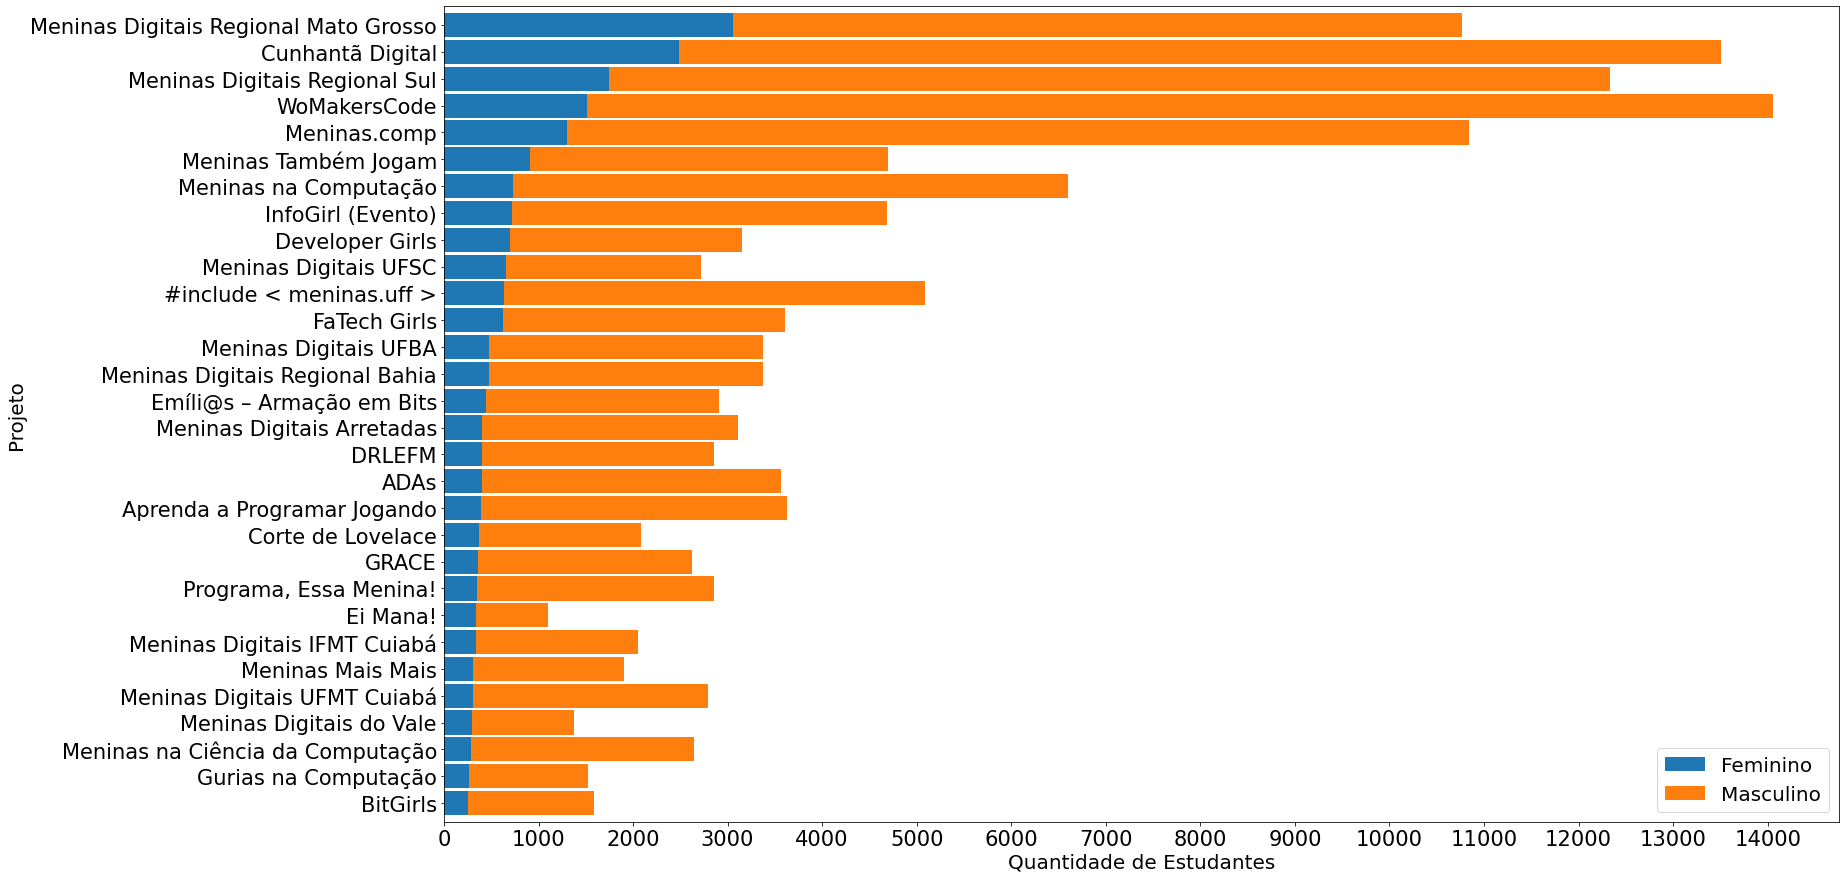
\includegraphics[width=1\textwidth]{Figuras/impacto_projetotrinta.png}
\caption{Número de estudantes possivelmente impactados por sexo e projeto}
\label{fig:impactoProjetoTotal}
\end{figure}

Como a descrição do que considera-se possível impacto, é nítido que o endereço, ano de início do projeto e quantidade de cursos classificados como TIC influenciam esta variável.

O gráfico da Figura \ref{fig:impactoAnoTotal} soma os possíveis impactos ano a ano. Observa-se uma crescente significativa a partir de 2014, e é possível relacionar com o número de projetos do Programa Meninas Digitais. Até o ano de 2014 existiam 13 projetos do Programa Meninas Digitais. Em 2015 mais 11 projetos foram iniciados, em 2016, 20 projetos foram iniciados, em 2017, 19 projetos, em 2018, 29 projetos e em 2019, 34 projetos. 


\begin{figure}[H]
\centering
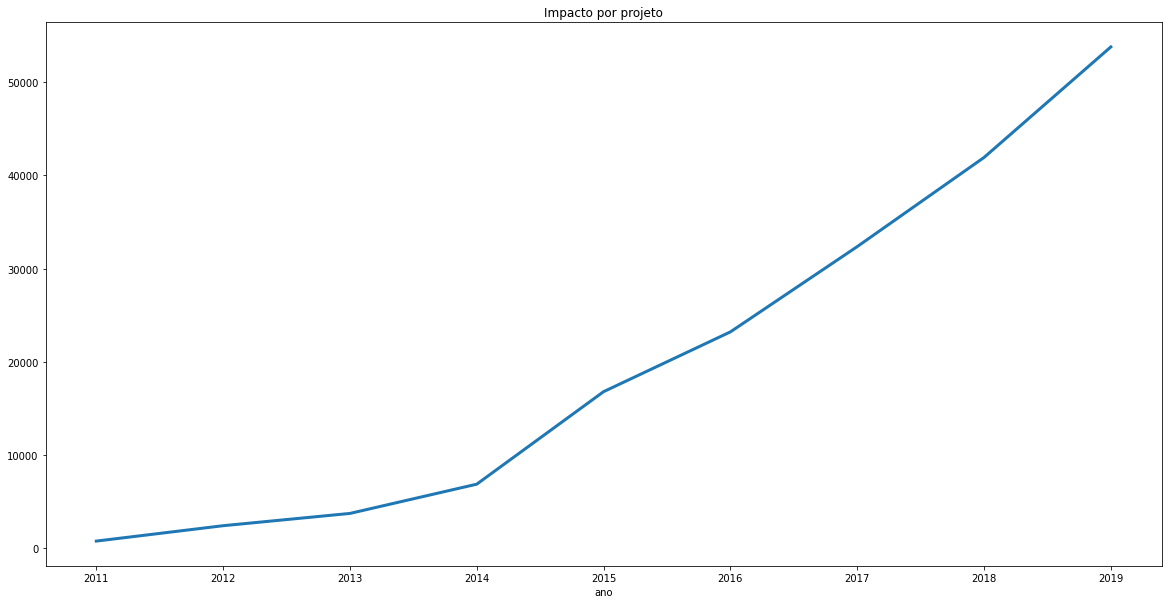
\includegraphics[width=1\textwidth]{Figuras/impactoanoTotal.png}
\caption{Número de estudantes possivelmente impactados por ano}
\label{fig:impactoAnoTotal}
\end{figure}




Já a Figura \ref{fig:idadeProjetos} apresenta o número de estudantes possivelmente impactados por sexo e idade de todos os projetos iniciados até 2019. É possível identificar a partir desta divisão por sexo que a média de idade das mulheres é levemente superior do que a idade dos homens, sendo aproximadamente 24,71 anos para a média feminina e 24,47 anos para os homens, que pode ser considerada igual. Já a mediana para ambos os sexos é de 23 anos. O pico das idades apresentam-se em 21 e 22 anos para ambos os sexos também.


\begin{figure}[H]
\centering
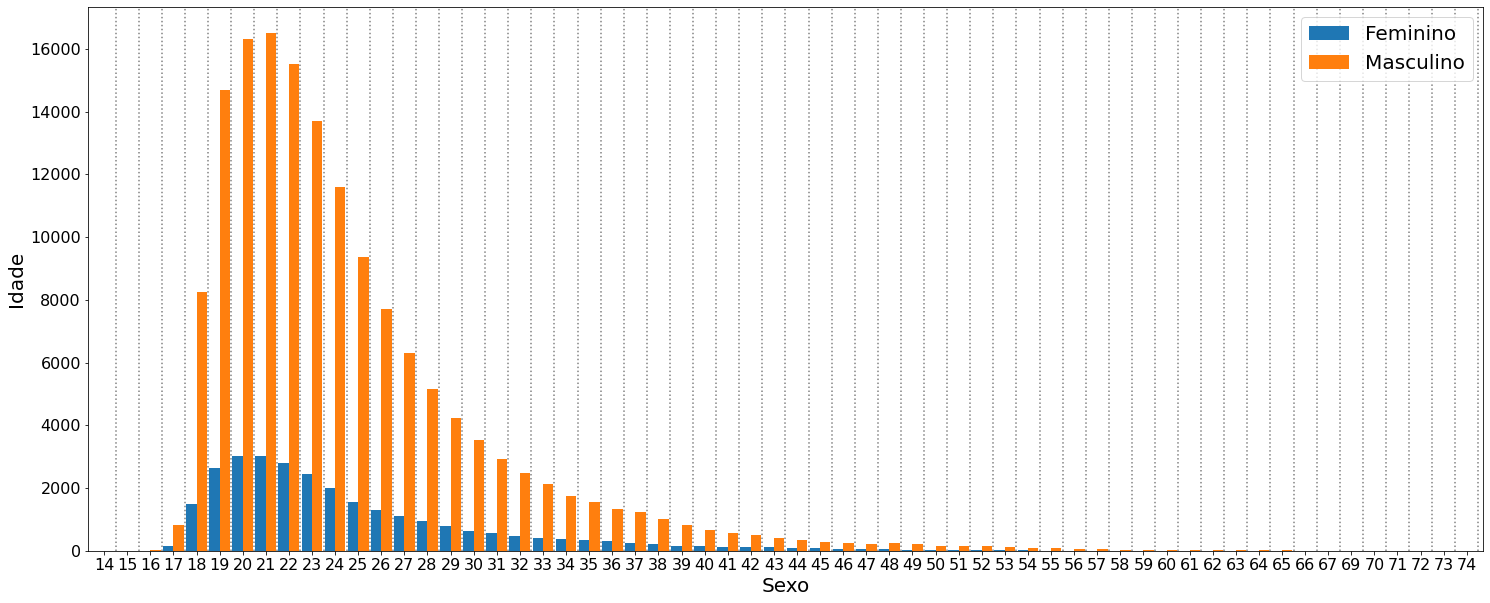
\includegraphics[width=1\textwidth]{Figuras/idadeProjetos.png}
\caption{Número de esetudantes possivelmente impactados categorizados por idade}
\label{fig:idadeProjetos}
\end{figure}








%\subsection{Projetos ativos}\label{sec:ProjetosAtivos}
%Após o levantamento dos projetos ativos, disponíveis no site Meninas Digitais, fez-se uma consulta ao comitê do programa para verificar os projetos ativos de fato, ou seja, os projetos que responderam ao questionário de participação ativa no ano de 2021. Chegando assim em um total de 72 projetos, que segundo a análise feita na Subseção \ref{sec:ProjetosLevantados} afeta então XX dos cursos XXXXXX (NOME DOS CURSOS 06 CINE).


\section{Projetos selecionados}\label{sec:ProjetosEscolhidos}

Por conta da pluralidade de projetos, foram selecionados 5 projetos a partir do possível impacto de cada um para exploração aprofundada. O impacto se dá pelo número de estudantes associados aos cursos e estudantes possivelmente afetados, com isso o gráfico da Figura \ref{fig:impactoProjetoTotal} explicita estes 5 projetos do programa Meninas Digitais. São eles WoMakersCode, Cunhantã Digital, Meninas Digitais Regional Sul, Meninas.Comp - Computação também é coisa de menina e Meninas Digitais Regional Mato Grosso do Sul.


% Please add the following required packages to your document preamble:
% \usepackage{multirow}
% \usepackage{graphicx}
% \usepackage[table,xcdraw]{xcolor}
% If you use beamer only pass "xcolor=table" option, i.e. \documentclass[xcolor=table]{beamer}
% \usepackage[normalem]{ulem}
% \useunder{\uline}{\ul}{}

% Please add the following required packages to your document preamble:
% \usepackage{multirow}
% \usepackage{graphicx}
% \usepackage[table,xcdraw]{xcolor}
% If you use beamer only pass "xcolor=table" option, i.e. \documentclass[xcolor=table]{beamer}
% \usepackage[normalem]{ulem}
% \useunder{\uline}{\ul}{}
\begin{table}[H]
\centering
\caption{Possível impacto por projetos selecionados}
\label{tab:ProjetosEscolhidos}
\resizebox{\textwidth}{!}{%
\begin{tabular}{|c|c|ccc|c|}
\hline
\rowcolor[HTML]{C0C0C0} 
\cellcolor[HTML]{C0C0C0}                     & \cellcolor[HTML]{C0C0C0}                                        & \multicolumn{3}{c|}{\cellcolor[HTML]{C0C0C0}Estudantes Possivelmente Impactados}                                    & \cellcolor[HTML]{C0C0C0}                         \\ \cline{3-5}
\rowcolor[HTML]{C0C0C0} 
\multirow{-2}{*}{\cellcolor[HTML]{C0C0C0}ID} & \multirow{-2}{*}{\cellcolor[HTML]{C0C0C0}Projetos Selecionados} & \multicolumn{1}{c|}{\cellcolor[HTML]{C0C0C0}Homens} & \multicolumn{1}{c|}{\cellcolor[HTML]{C0C0C0}Mulheres} & Total & \multirow{-2}{*}{\cellcolor[HTML]{C0C0C0}Início} \\ \hline
1                                            & WoMakersCode                                                    & \multicolumn{1}{c|}{12542}                          & \multicolumn{1}{c|}{1509}                             & 14051 & 2015                                             \\ \hline
2                                            & Cunhatã Digital                                                 & \multicolumn{1}{c|}{11017}                          & \multicolumn{1}{c|}{2488}                             & 13505 & 2015                                             \\ \hline
3                                            & Meninas Digitais Regional Sul                                   & \multicolumn{1}{c|}{10578}                          & \multicolumn{1}{c|}{1749}                             & 12327 & 2012                                             \\ \hline
4                                            & Meninas.Comp                                                    & \multicolumn{1}{c|}{9540}                           & \multicolumn{1}{c|}{1306}                             & 10846 & 2011                                             \\ \hline
5                                            & Meninas Digitais Regional Mato Grosso                           & \multicolumn{1}{c|}{7712}                           & \multicolumn{1}{c|}{3060}                             & 10772 & 2015                                             \\ \hline
\end{tabular}%
}
\end{table}



Dos 5 projetos escolhidos, cada um consecutivamente possivelmente afetam 7, 11, 3,3,3 cursos de TIC. A coluna ID da Tabela \ref{tab:ProjetosEscolhidosComCurso} relaciona-se com a coluna ID da Tabela \ref{fig:impactoProjetoTotal} para identificação de cada projeto. Os cursos, IES e seus códigos são apresentados na Tabela \ref{tab:ProjetosEscolhidosComCurso}.

\begin{longtable}[c]{|c|c|c|c|c|}
\caption{Cursos e IES relacionadas com os projetos selecionados}
\label{tab:ProjetosEscolhidosComCurso}\\
\hline
\rowcolor[HTML]{C0C0C0} 
\textbf{ID}          & \textbf{Código IES}    & \textbf{Nome IES}                                                                                                                  & \textbf{Código Curso}    & \textbf{Nome Curso}                                                                \\ \hline
\endfirsthead
%
\multicolumn{5}{c}%
{{\bfseries Tabela \thetable\ continuação da página anterior}} \\
\hline
\rowcolor[HTML]{C0C0C0} 
\textbf{ID}          & \textbf{Código IES}    & \textbf{Nome IES}                                                                                                                  & \textbf{Código Curso}    & \textbf{Nome Curso}                                                                \\ \hline
\endhead
%
                     &                        &                                                                                                                                    & 1904                     & Ciência da Computação                                                              \\ \cline{4-5} 
                     &                        &                                                                                                                                    & 56702                    & Engenharia da Computação                                                           \\ \cline{4-5} 
                     &                        &                                                                                                                                    & 56766                    & Sistemas de Informação                                                             \\ \cline{4-5} 
                     & \multirow{-4}{*}{21}   & \multirow{-4}{*}{\begin{tabular}[c]{@{}c@{}}Pontifícia \\ Universidade Católica\\  do Rio Grande do Sul\end{tabular}}              & 1314299                  & Engenharia de Software                                                             \\ \cline{2-5} 
                     &                        &                                                                                                                                    & 83904                    & \begin{tabular}[c]{@{}c@{}}Engenharia de Computação \\ e Informação\end{tabular}   \\ \cline{4-5} 
                     & \multirow{-2}{*}{586}  & \multirow{-2}{*}{\begin{tabular}[c]{@{}c@{}}Universidade Federal \\ do Rio de Janeiro\end{tabular}}                                & 85783                    & Ciência da Computação                                                              \\ \cline{2-5} 
\multirow{-7}{*}{1}  & 2950                   & \begin{tabular}[c]{@{}c@{}}Centro Universitário \\ FADERGS\end{tabular}                                                            & 1282899                  & Ciência da Computação                                                              \\ \hline
                     &                        &                                                                                                                                    & 62484                    & Ciência da Computação                                                              \\ \cline{4-5} 
                     &                        &                                                                                                                                    & 112086                   & Sistemas de Informação                                                             \\ \cline{4-5} 
                     &                        &                                                                                                                                    & 122634                   & Engenharia de Software                                                             \\ \cline{4-5} 
                     & \multirow{-4}{*}{4}    & \multirow{-4}{*}{\begin{tabular}[c]{@{}c@{}}Universidade Federal \\ do Amazonas\end{tabular}}                                      & 1158678                  & Engenharia de Software                                                             \\ \cline{2-5} 
                     &                        &                                                                                                                                    & 17886                    & Sistemas de Informação                                                             \\ \cline{4-5} 
                     &                        &                                                                                                                                    & 22061                    & Ciência da Computação                                                              \\ \cline{4-5} 
                     &                        &                                                                                                                                    & 110564                   & Engenharia de Computação                                                           \\ \cline{4-5} 
                     & \multirow{-4}{*}{1049} & \multirow{-4}{*}{\begin{tabular}[c]{@{}c@{}}Instituto de Ensino \\ Superior FUCAPI\end{tabular}}                                   & 1261039                  & Engenharia de Software                                                             \\ \cline{2-5} 
                     &                        &                                                                                                                                    & 69318                    & \begin{tabular}[c]{@{}c@{}}Análise e Desenvolvimento\\ de Sistemas\end{tabular}    \\ \cline{4-5} 
                     &                        &                                                                                                                                    & 1330347                  & Sistemas de Informação                                                             \\ \cline{4-5} 
\multirow{-11}{*}{2} & \multirow{-3}{*}{3172} & \multirow{-3}{*}{\begin{tabular}[c]{@{}c@{}}Universidade do Estado\\ do Amazonas\end{tabular}}                                     & 1330348                  & Jogos Digitais                                                                     \\ \hline
                     &                        &                                                                                                                                    & 14217                    & Ciência da Computação                                                              \\ \cline{4-5} 
                     &                        &                                                                                                                                    & 21600                    & Sistemas de Informação                                                             \\ \cline{4-5} 
\multirow{-1}{*}{3}  & \multirow{-1}{*}{585}  & \multirow{-1.5}{*}{\begin{tabular}[c]{@{}c@{}}Universidade Federal\\ de Santa Catarina\end{tabular}}                                 & 1084054                  & \begin{tabular}[c]{@{}c@{}}Tecnologias da Informação\\  e Comunicação\end{tabular} \\ \hline
                     &                        &                                                                                                                                    & 127                      & Ciência da Computação                                                              \\ \cline{4-5} 
                     &                        &                                                                                                                                    & 112891                   & Engenharia de Software                                                             \\ \cline{4-5} 
\multirow{-3}{*}{4}  & \multirow{-3}{*}{2}    & \multirow{-3}{*}{\begin{tabular}[c]{@{}c@{}}Universidade \\ de Brasília\end{tabular}}                                              & 122204                   & Engenharia de Computação                                                           \\ \hline
                     &                        &                                                                                                                                    & 65473                    & Sistemas para Internet                                                             \\ \cline{4-5} 
                     &                        &                                                                                                                                    & 90361                    & Redes de Computadores                                                              \\ \cline{4-5} 
                     &                        &                                                                                                                                    &                          &                                                                                    \\
\multirow{-4}{*}{5}  & \multirow{-4}{*}{3164} & \multirow{-4}{*}{\begin{tabular}[c]{@{}c@{}}Instituto Federal\\ de Educação, Ciência\\ e Tecnologia de\\ Mato Grosso\end{tabular}} & \multirow{-2}{*}{100694} & \multirow{-2}{*}{Sistemas para Internet}                                           \\ \hline
\end{longtable}

%Como todos os projetos presentes no site levantados tiveram sua última atualização no ano de 2020, decidiu-se por contatar o Programa Meninas Digitais e com isso uma tabela mais atual contendo apenas os projetos ativos no ano de 2022 com nome do projeto, cidade e ano de início foi disponibilizada e podem ser identificados pelas linhas coloridas da Tabela \ref{tab:ProjetosMeninasDigitais}. Alguns projetos disponíveis nesta planilha não constavam no site no dia da busca, por isso não foram considerados para esta pesquisa, são eles AI Girls - São Paulo (2020), IT Girls - Rio Tinto (2015), Meninas++ - Rio Paranaíba (2012), Minatech - Florianópolis (2021) e Projeto ADAs - Goiânia (2017). Apesar disso, os 5 projetos que possivelmente mais impactam pessoas não modificam-se, pois todos eram de fato projetos ativos e estavam contidos nessa atualização.

Com os projetos apresentados na Tabela \ref{tab:ProjetosEscolhidosComCurso} análises mais individuais são propostas na Seção \ref{sec:Avaliacoes} para entendimento da evasão no contexto desses projetos. 

\section{Análises}\label{sec:Avaliacoes}

As análises presentes nessa seção utilizam-se apenas dos dados do INEP relativos aos 5 projetos e aos 27 cursos que relacionam-se com tais projetos, descritos na Tabela \ref{tab:ProjetosEscolhidosComCurso}.

As Figuras \ref{fig:calorCorRaca}, \ref{fig:calorFormaIngresso} e \ref{fig:calorIdade} são gráficos de calor com a evolução anual da evasão de acordo com os parâmetros de cor e raça, forma de ingresso e idade dos estudantes possivelmente envolvidos nos projetos selecionados.
É importante neste ponto relembrar que a Equação utilizada para o cálculo da evasão está disponível na Seção \ref{sec:CalculoEvasao}.


As análises apresentadas foram feitas a partir de dados fornecidos pelo INEP. Todas as análises baseiam-se na divisão de gênero disponível no banco de dados, as variáveis mostradas são apenas feminino e masculino, bem como todas as outras divisões de cor e raça e forma de ingresso.

INÍCIO ANÁLISES NOVAS:

\begin{figure}[H]
\centering
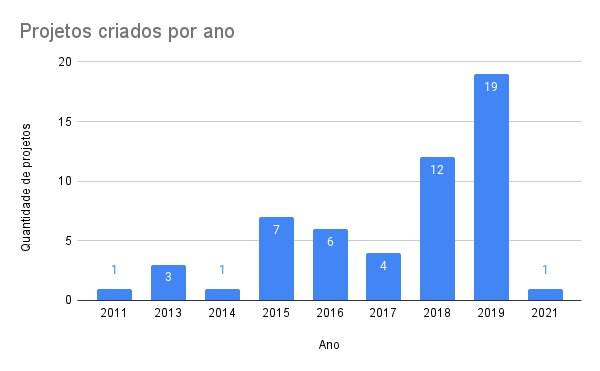
\includegraphics[width=1\textwidth]{Figuras/ProjetosPorAno.jpeg}
\caption{---}
\label{fig:ProjetosPorAno}
\end{figure}
 
\begin{figure}[H]
\centering
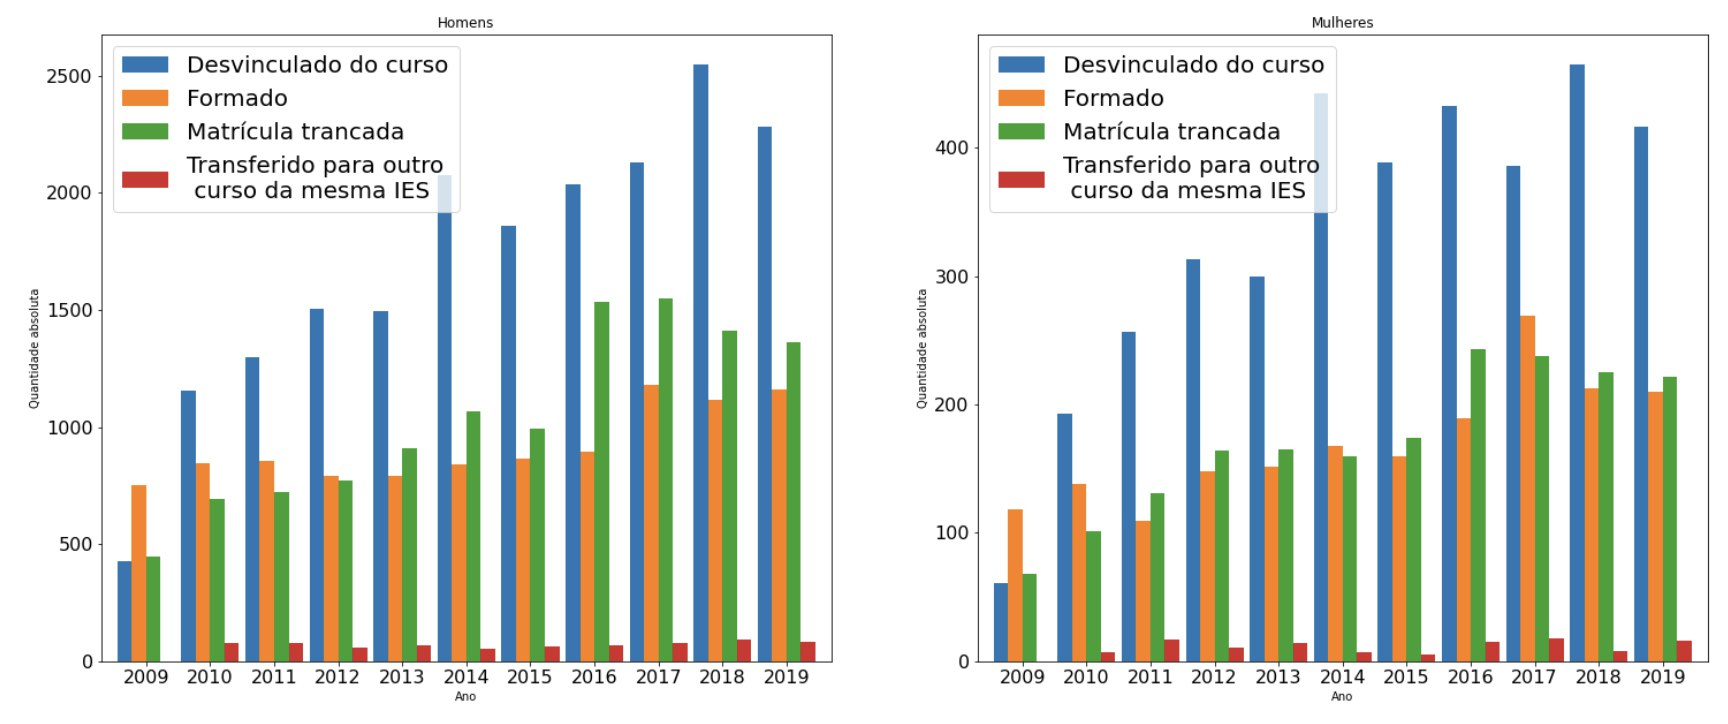
\includegraphics[width=1\textwidth]{Figuras/situacaodosalunos.jpeg}
\caption{---}
\label{fig:situacaodosalunos}
\end{figure}

\begin{figure}[H]
\centering
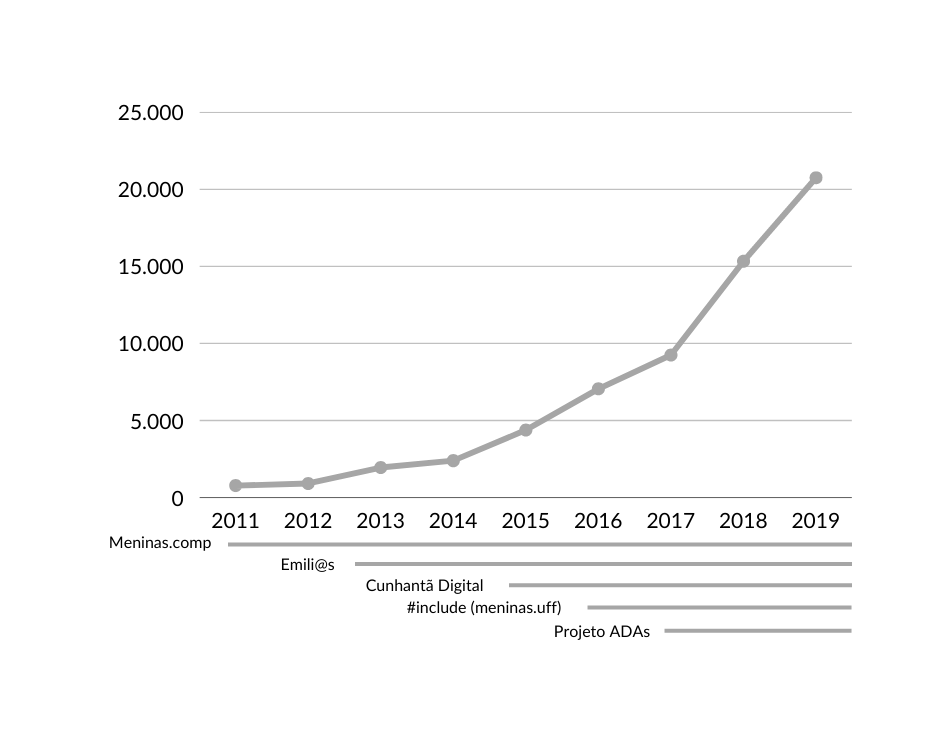
\includegraphics[width=1\textwidth]{Figuras/numeroalunosprojeto.png}
\caption{---}
\label{fig:numeroalunosprojeto}
\end{figure}


\begin{figure}[H]
\centering
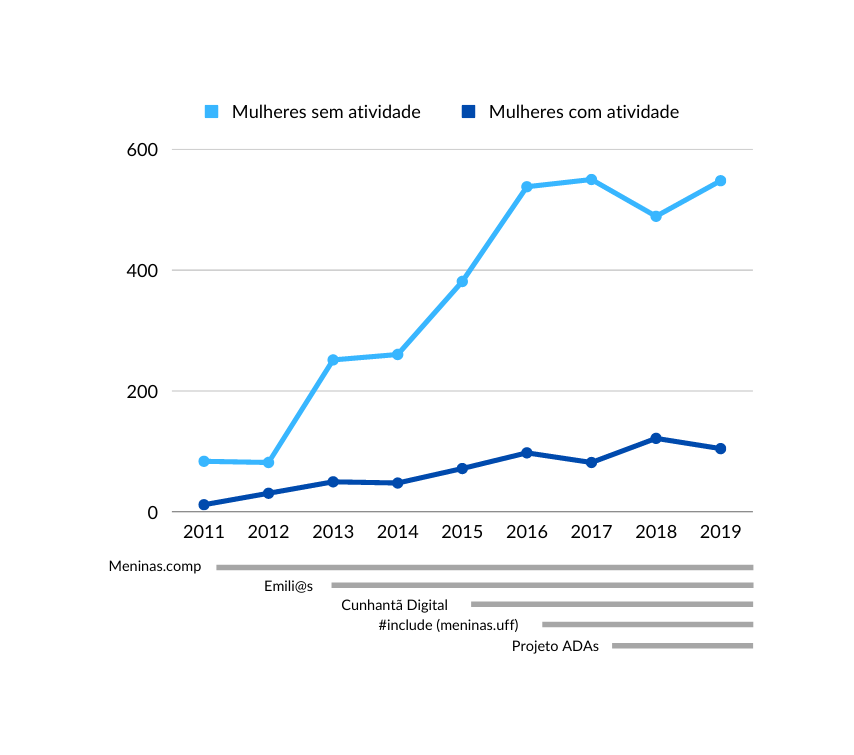
\includegraphics[width=1\textwidth]{Figuras/atividadeextra.png}
\caption{---}
\label{fig:atividadeextra}
\end{figure}


\begin{figure}[H]
\centering
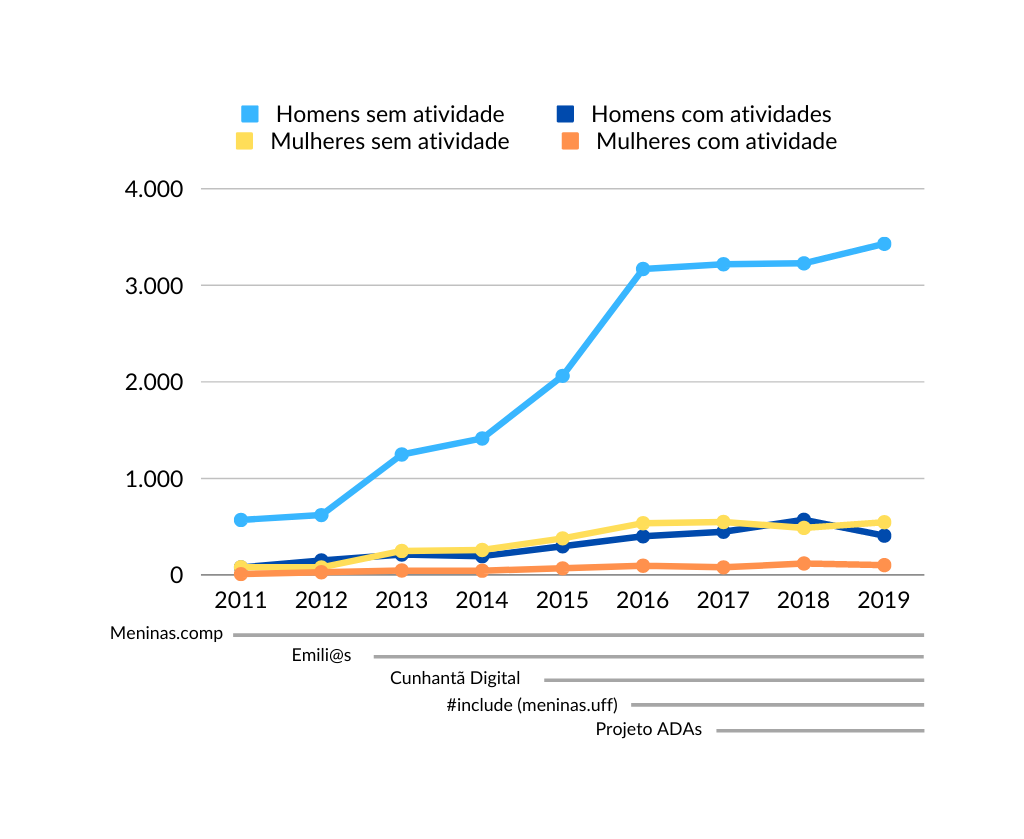
\includegraphics[width=1\textwidth]{Figuras/quantidadeatividadeextra.png}
\caption{---}
\label{fig:quantidadeatividadeextra}
\end{figure}


FIM ANÁLISES NOVAS


\subsection{Evasão por Ano, Cor e Raça}\label{sub:calorCorERaca}
A Figura \ref{fig:calorCorRaca} apresenta as informações quanto ao gênero, raça e taxa de evasão. Percebe-se que a evasão máxima em porcentagem acontece no ano de 2012 onde 75\% das mulheres que não quiseram declarar sua cor e raça evadiram. Embora preocupante, esse valor é atrelado a baixa quantidade de mulheres pertencentes a esse grupo.

Além disso, há vários pontos onde a taxa de evasão é zerada, significando que, dos estudantes evadidos daquele período, nenhum pertencia ao determinado grupo. Vale ressaltar que alguns campos estão sem informações pois não haviam estudantes nesse grupo e período.


\begin{figure}[H]
\centering
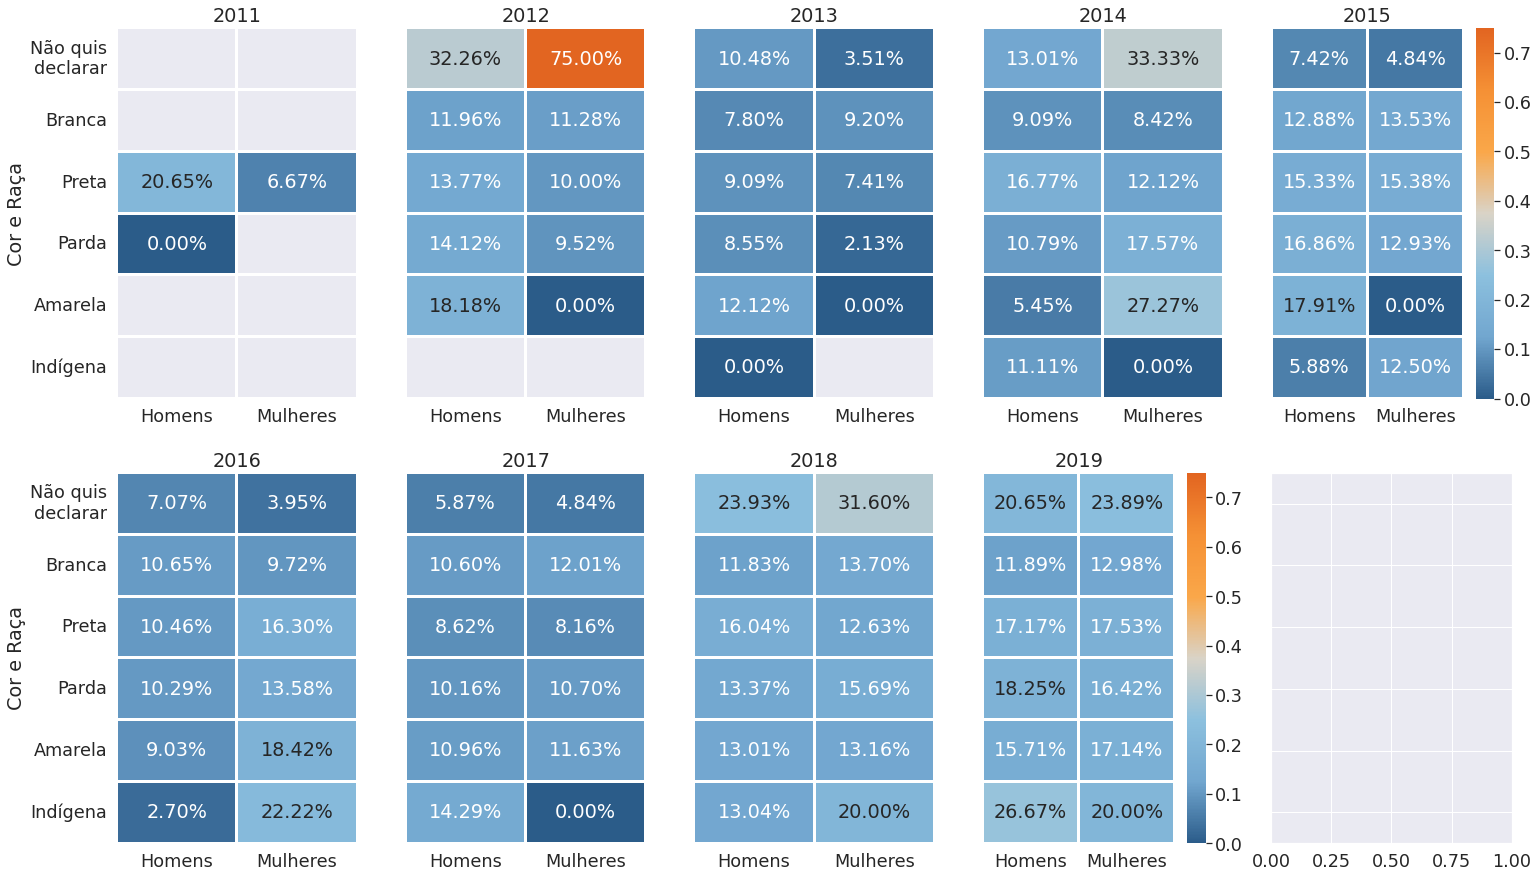
\includegraphics[width=1\textwidth]{Figuras/calorCorRaca.png}
\caption{Evasão do conjunto de projetos selecionados por ano, cor e raça}
\label{fig:calorCorRaca}
\end{figure}

No decorrer de todos os anos nenhum dos grupos apresentou alta contínua ou queda continua, mas é interessante observar o comportamento das indígenas, que variam entre zero e aproximadamente 20\% de um ano para outro, reforçando que o número de mulheres indígenas é baixo e com apenas uma evasão a taxa sobe significativamente.

Apesar de nenhum grupo apresentar queda ou crescente contínua para todos os anos, todos os grupos apresentam queda no ano de 2012 para 2013. De 2015 a 2016 todos os homens apresentaram queda na taxa de evasão e apenas as mulheres que não quiseram declarar e as brancas seguiram esta tendência, o restante do grupo teve um aumento na taxa de evasão.

Em uma visão com valores absolutos apresentadas nas Tabelas \ref{tab:numabsoluto2011}, \ref{tab:numabsoluto2014} e \ref{tab:numabsoluto2017} onde observa-se que em nenhum dos grupos o número de homens é inferior ao número de mulheres. Lembrando que os valores absolutos de estudantes não trazem uma relação direta com a evasão, pois por exemplo, o número de estudantes mulheres amarelas pode ter permanecido o mesmo em dois anos distintos ou até aumentado, mas todas as mulheres do ano X podem ter evadido em X+1 e X+1 pode apresentar mulheres distintas ingressantes, tendo assim uma taxa de evasão elevada.


\begin{table}[H]
\caption{Número absoluto de estudantes por ano, gênero, cor e raça de 2011 a 2013}
\label{tab:numabsoluto2011}
\resizebox{\textwidth}{!}{%
\begin{tabular}{c|cc|cc|cc|}
\cline{2-7}
                                                                         & \multicolumn{2}{c|}{\cellcolor[HTML]{C0C0C0}\textbf{2011}}                                               & \multicolumn{2}{c|}{\cellcolor[HTML]{C0C0C0}\textbf{2012}}                                               & \multicolumn{2}{c|}{\cellcolor[HTML]{C0C0C0}\textbf{2013}}                                               \\ \cline{2-7} 
\multirow{-2}{*}{}                                                       & \multicolumn{1}{c|}{\cellcolor[HTML]{C0C0C0}\textbf{Homens}} & \cellcolor[HTML]{C0C0C0}\textbf{Mulheres} & \multicolumn{1}{c|}{\cellcolor[HTML]{C0C0C0}\textbf{Homens}} & \cellcolor[HTML]{C0C0C0}\textbf{Mulheres} & \multicolumn{1}{c|}{\cellcolor[HTML]{C0C0C0}\textbf{Homens}} & \cellcolor[HTML]{C0C0C0}\textbf{Mulheres} \\ \hline
\multicolumn{1}{|c|}{\cellcolor[HTML]{C0C0C0}\textbf{Não quis declarar}} & \multicolumn{1}{c|}{0}                                       & 0                                         & \multicolumn{1}{c|}{31}                                      & 4                                         & \multicolumn{1}{c|}{301}                                     & 54                                        \\ \hline
\multicolumn{1}{|c|}{\cellcolor[HTML]{C0C0C0}\textbf{Branca}}            & \multicolumn{1}{c|}{0}                                       & 0                                         & \multicolumn{1}{c|}{1129}                                    & 195                                       & \multicolumn{1}{c|}{1389}                                    & 220                                       \\ \hline
\multicolumn{1}{|c|}{\cellcolor[HTML]{C0C0C0}\textbf{Preta}}             & \multicolumn{1}{c|}{92}                                      & 15                                        & \multicolumn{1}{c|}{143}                                     & 28                                        & \multicolumn{1}{c|}{104}                                     & 23                                        \\ \hline
\multicolumn{1}{|c|}{\cellcolor[HTML]{C0C0C0}\textbf{Parda}}             & \multicolumn{1}{c|}{1}                                       & 0                                         & \multicolumn{1}{c|}{85}                                      & 21                                        & \multicolumn{1}{c|}{249}                                     & 45                                        \\ \hline
\multicolumn{1}{|c|}{\cellcolor[HTML]{C0C0C0}\textbf{Amarela}}           & \multicolumn{1}{c|}{0}                                       & 0                                         & \multicolumn{1}{c|}{11}                                      & 2                                         & \multicolumn{1}{c|}{29}                                      & 8                                         \\ \hline
\multicolumn{1}{|c|}{\cellcolor[HTML]{C0C0C0}\textbf{Indígena}}          & \multicolumn{1}{c|}{0}                                       & 0                                         & \multicolumn{1}{c|}{0}                                       & 0                                         & \multicolumn{1}{c|}{1}                                       & 0                                         \\ \hline
\end{tabular}%
}
\end{table}

\begin{table}[H]
\caption{Número absoluto de estudantes por ano, gênero, cor e raça de 2014 a 2016}
\label{tab:numabsoluto2014}
\resizebox{\textwidth}{!}{%
\begin{tabular}{c|cc|cc|cc|}
\cline{2-7}
                                                                         & \multicolumn{2}{c|}{\cellcolor[HTML]{C0C0C0}\textbf{2014}}                                               & \multicolumn{2}{c|}{\cellcolor[HTML]{C0C0C0}\textbf{2015}}                                               & \multicolumn{2}{c|}{\cellcolor[HTML]{C0C0C0}\textbf{2016}}                                               \\ \cline{2-7} 
\multirow{-2}{*}{}                                                       & \multicolumn{1}{c|}{\cellcolor[HTML]{C0C0C0}\textbf{Homens}} & \cellcolor[HTML]{C0C0C0}\textbf{Mulheres} & \multicolumn{1}{c|}{\cellcolor[HTML]{C0C0C0}\textbf{Homens}} & \cellcolor[HTML]{C0C0C0}\textbf{Mulheres} & \multicolumn{1}{c|}{\cellcolor[HTML]{C0C0C0}\textbf{Homens}} & \cellcolor[HTML]{C0C0C0}\textbf{Mulheres} \\ \hline
\multicolumn{1}{|c|}{\cellcolor[HTML]{C0C0C0}\textbf{Não quis declarar}} & \multicolumn{1}{c|}{96}                                      & 15                                        & \multicolumn{1}{c|}{1362}                                    & 489                                       & \multicolumn{1}{c|}{1280}                                    & 475                                       \\ \hline
\multicolumn{1}{|c|}{\cellcolor[HTML]{C0C0C0}\textbf{Branca}}            & \multicolumn{1}{c|}{1601}                                    & 254                                       & \multicolumn{1}{c|}{4265}                                    & 649                                       & \multicolumn{1}{c|}{4324}                                    & 634                                       \\ \hline
\multicolumn{1}{|c|}{\cellcolor[HTML]{C0C0C0}\textbf{Preta}}             & \multicolumn{1}{c|}{145}                                     & 31                                        & \multicolumn{1}{c|}{364}                                     & 70                                        & \multicolumn{1}{c|}{399}                                     & 75                                        \\ \hline
\multicolumn{1}{|c|}{\cellcolor[HTML]{C0C0C0}\textbf{Parda}}             & \multicolumn{1}{c|}{382}                                     & 72                                        & \multicolumn{1}{c|}{2202}                                    & 511                                       & \multicolumn{1}{c|}{2328}                                    & 508                                       \\ \hline
\multicolumn{1}{|c|}{\cellcolor[HTML]{C0C0C0}\textbf{Amarela}}           & \multicolumn{1}{c|}{49}                                      & 11                                        & \multicolumn{1}{c|}{129}                                     & 31                                        & \multicolumn{1}{c|}{113}                                     & 37                                        \\ \hline
\multicolumn{1}{|c|}{\cellcolor[HTML]{C0C0C0}\textbf{Indígena}}          & \multicolumn{1}{c|}{9}                                       & 2                                         & \multicolumn{1}{c|}{31}                                      & 7                                         & \multicolumn{1}{c|}{30}                                      & 8                                         \\ \hline
\end{tabular}%
}
\end{table}

\begin{table}[H]
\caption{Número absoluto de estudantes por ano, gênero, cor e raça de 2017 a 2019}
\label{tab:numabsoluto2017}
\resizebox{\textwidth}{!}{%
\begin{tabular}{c|cc|cc|cc|}
\cline{2-7}
                                                                         & \multicolumn{2}{c|}{\cellcolor[HTML]{C0C0C0}\textbf{2017}}                                               & \multicolumn{2}{c|}{\cellcolor[HTML]{C0C0C0}\textbf{2018}}                                               & \multicolumn{2}{c|}{\cellcolor[HTML]{C0C0C0}\textbf{2019}}                                               \\ \cline{2-7} 
\multirow{-2}{*}{}                                                       & \multicolumn{1}{c|}{\cellcolor[HTML]{C0C0C0}\textbf{Homens}} & \cellcolor[HTML]{C0C0C0}\textbf{Mulheres} & \multicolumn{1}{c|}{\cellcolor[HTML]{C0C0C0}\textbf{Homens}} & \cellcolor[HTML]{C0C0C0}\textbf{Mulheres} & \multicolumn{1}{c|}{\cellcolor[HTML]{C0C0C0}\textbf{Homens}} & \cellcolor[HTML]{C0C0C0}\textbf{Mulheres} \\ \hline
\multicolumn{1}{|c|}{\cellcolor[HTML]{C0C0C0}\textbf{Não quis declarar}} & \multicolumn{1}{c|}{1600}                                    & 597                                       & \multicolumn{1}{c|}{1461}                                    & 513                                       & \multicolumn{1}{c|}{1109}                                    & 321                                       \\ \hline
\multicolumn{1}{|c|}{\cellcolor[HTML]{C0C0C0}\textbf{Branca}}            & \multicolumn{1}{c|}{4430}                                    & 656                                       & \multicolumn{1}{c|}{4400}                                    & 626                                       & \multicolumn{1}{c|}{4243}                                    & 604                                       \\ \hline
\multicolumn{1}{|c|}{\cellcolor[HTML]{C0C0C0}\textbf{Preta}}             & \multicolumn{1}{c|}{458}                                     & 81                                        & \multicolumn{1}{c|}{471}                                     & 80                                        & \multicolumn{1}{c|}{452}                                     & 81                                        \\ \hline
\multicolumn{1}{|c|}{\cellcolor[HTML]{C0C0C0}\textbf{Parda}}             & \multicolumn{1}{c|}{2569}                                    & 542                                       & \multicolumn{1}{c|}{2704}                                    & 568                                       & \multicolumn{1}{c|}{2658}                                    & 549                                       \\ \hline
\multicolumn{1}{|c|}{\cellcolor[HTML]{C0C0C0}\textbf{Amarela}}           & \multicolumn{1}{c|}{125}                                     & 34                                        & \multicolumn{1}{c|}{123}                                     & 28                                        & \multicolumn{1}{c|}{109}                                     & 29                                        \\ \hline
\multicolumn{1}{|c|}{\cellcolor[HTML]{C0C0C0}\textbf{Indígena}}          & \multicolumn{1}{c|}{39}                                      & 6                                         & \multicolumn{1}{c|}{38}                                      & 5                                         & \multicolumn{1}{c|}{38}                                      & 4                                         \\ \hline
\end{tabular}%
}
\end{table}


\subsection{Evasão por Ano e Forma de Ingresso}\label{sub:calorFomaIngresso}

Para a apresentação do gráfico da Figura \ref{fig:calorFormaIngresso}, as categorias não nulas presentes na base de dados são referentes a forma com que o estudante ingressou na IES e são identificadas por:
\begin{itemize}
    \item Enem: Informa se o estudante ingressou no curso pelo Enem;
    \item Ensino Público:  Informa se o estudante ingressou por meio de programa de reserva de vagas para egressos da escola pública;
    \item Renda Familiar: Informa se o estudante ingressou por meio de programa de reserva de vagas de cunho social ou de renda familiar;
    \item Reserva de Vagas: Informa se o estudante participa de programa de reserva de vagas;
    \item Seleção Simplificada: Informa se o estudante ingressou no curso por meio de seleção simplificada;
    \item Vagas Remanescentes: Informa se o estudante ingressou no curso por meio de vagas remanescentes;
    \item Vagas Étnicas: Informa se o estudante ingressou por meio de programa de reserva de vagas de cunho étnico;
    \item Vestibular: Informa se o estudante ingressou no curso pelo vestibular.
\end{itemize}

A análise das formas de ingresso nas instituições citadas presente na Figura \ref{fig:calorFormaIngresso}, relacionando-se com gênero e taxa de evasão por ano, desde 2011 até 2019. O ponto onde o gráfico possui a maior taxa de evasão pertence ao ano de 2014, onde, dos homens que ingressaram pelo programa de renda familiar, 33,33\% evadiram. Já com as estudantes mulheres, a maior porcentagem está no ano de 2018 onde 26,09\% que ingressaram pelo programa de seleção simplificada evadiram. 

\begin{figure}[H]
\centering
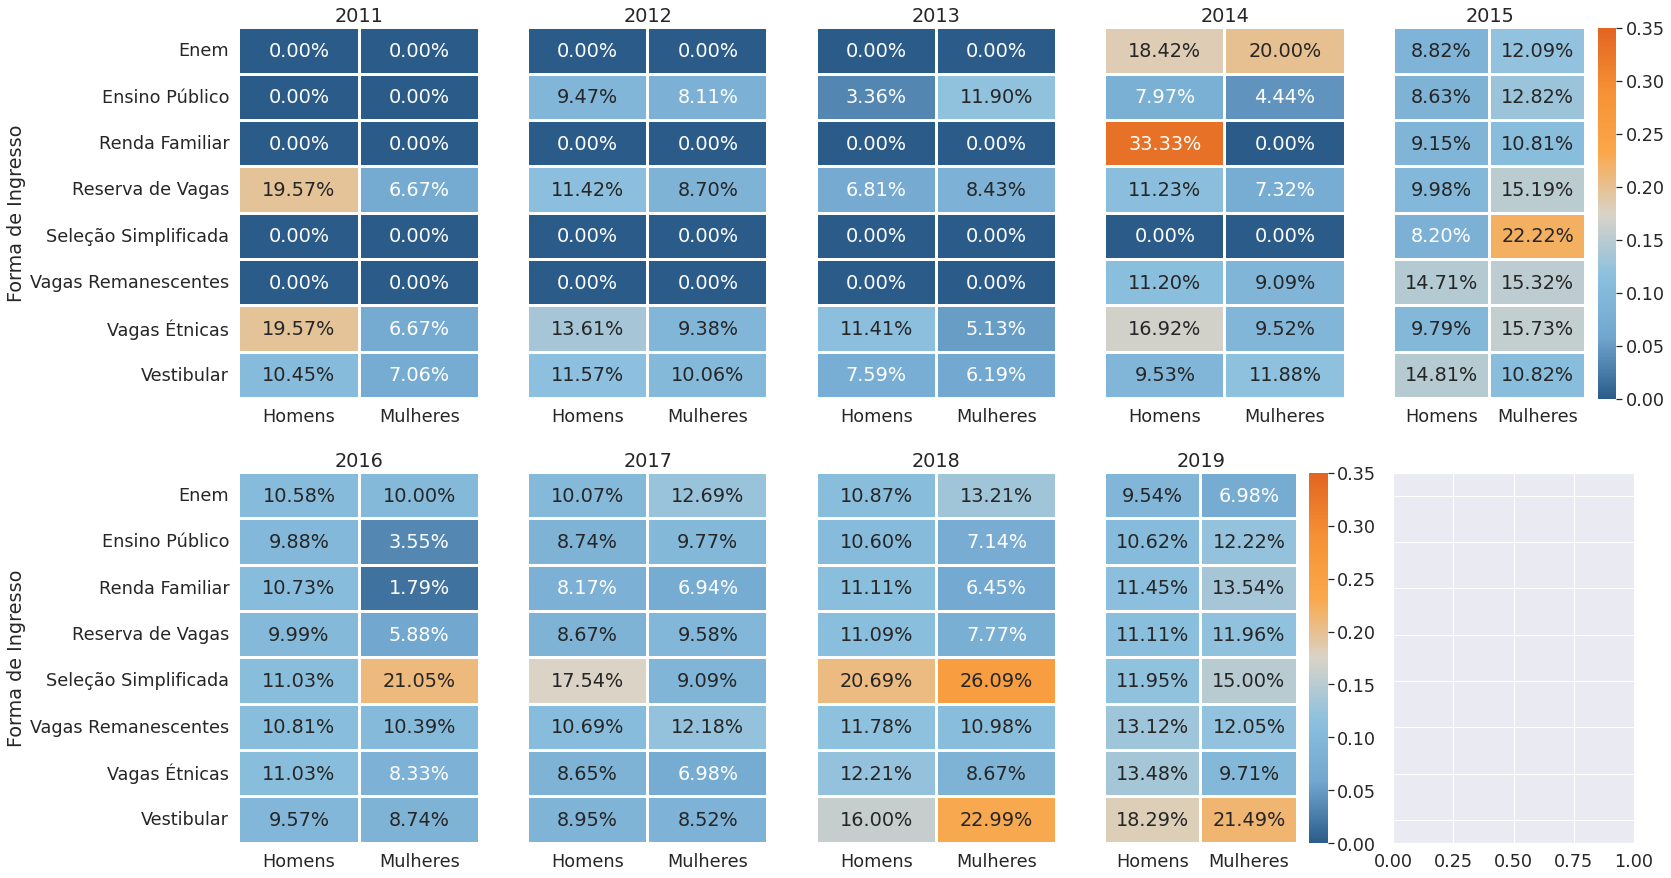
\includegraphics[width=1\textwidth]{Figuras/calorFormaIngresso.png}
\caption{Evasão do conjunto de projetos selecionados por ano e forma de ingresso}
\label{fig:calorFormaIngresso}
\end{figure}

É possível observar também que apresentam maior frequência de valores altos para da taxa de evasão as mulheres que ingressaram por seleção simplificada, onde inicialmente apresentavam taxa zero até o ano de 2014. Em números absolutos em ordem crescente de anos iniciando em 2011, o número de mulheres que ingressaram nas IES pela seleção simplificada foi 0, 0, 0, 0, 18, 15, 18, 20 e 14.

Também é possível observar todos os homens e mulheres que ingressaram por meio do vestibular e vagas étnicas entre os anos de 2017, 2018 e 2019 apresentaram alta na porcentagem de evasão.


\subsection{Evasão por Ano e Idade}\label{sub:calorIdade}
%COLOCAR ALGO ASSIM:
%No conjunto de dados observado, a diferença de idade máxima encontrada entre homens e mulheres foi bastante significativa, sendo 61 anos para homens e 48 anos para mulheres. Essa faixa etária, porém, é pouco presente no curso, que possui estudantes com uma idade média de 22 anos, tanto para homens quanto para mulheres. Portanto, considerando os dados anteriores, o intervalo de análise mínimo proposto foi de até 25 anos, com intervalo máximo de mais de 55 anos. 


A Figura \ref{fig:calorIdade} apresenta a relação entre gênero, idade e taxa de evasão nos anos observados. Um dos pontos críticos, onde houve maior evasão do gráfico ocorreu em 2012, em que, considerando apenas o número total de homens com idade maior de 55 anos, 66,67\% daqueles que estavam nessa faixa etária evadiram. Para mulheres, o ponto de máxima porcentagem ocorreu nos anos de 2013 e 2018, na faixa etária de maior de 55 anos, em que 50\% das mulheres contidas nessa faixa de idade evadiram. Observa-se nos extremos do gráfico, ou seja nas menores idades e maiores idades, um grande número de porcentagens zeradas, pois nessa faixa etária o número de estudantes mostra-se reduzido, fazendo com que cada estudante evadido tenha uma grande alta na porcentagem bem como quando nenhum estudante evade o que faz com que a taxa fique zerada.

Além disso, percebe-se que as menores taxas de evasão são de estudantes com faixa etária de até 25 anos. É importante pontuar que quadrados que não possuem a porcentagem de evasão e aparecem sem cor estão dessa forma pois nos anos analisados não haviam estudantes naquela faixa etária, e portanto não é possível concluir sobre a taxa de evasão para a mesma. 


\begin{figure}[H]
\centering
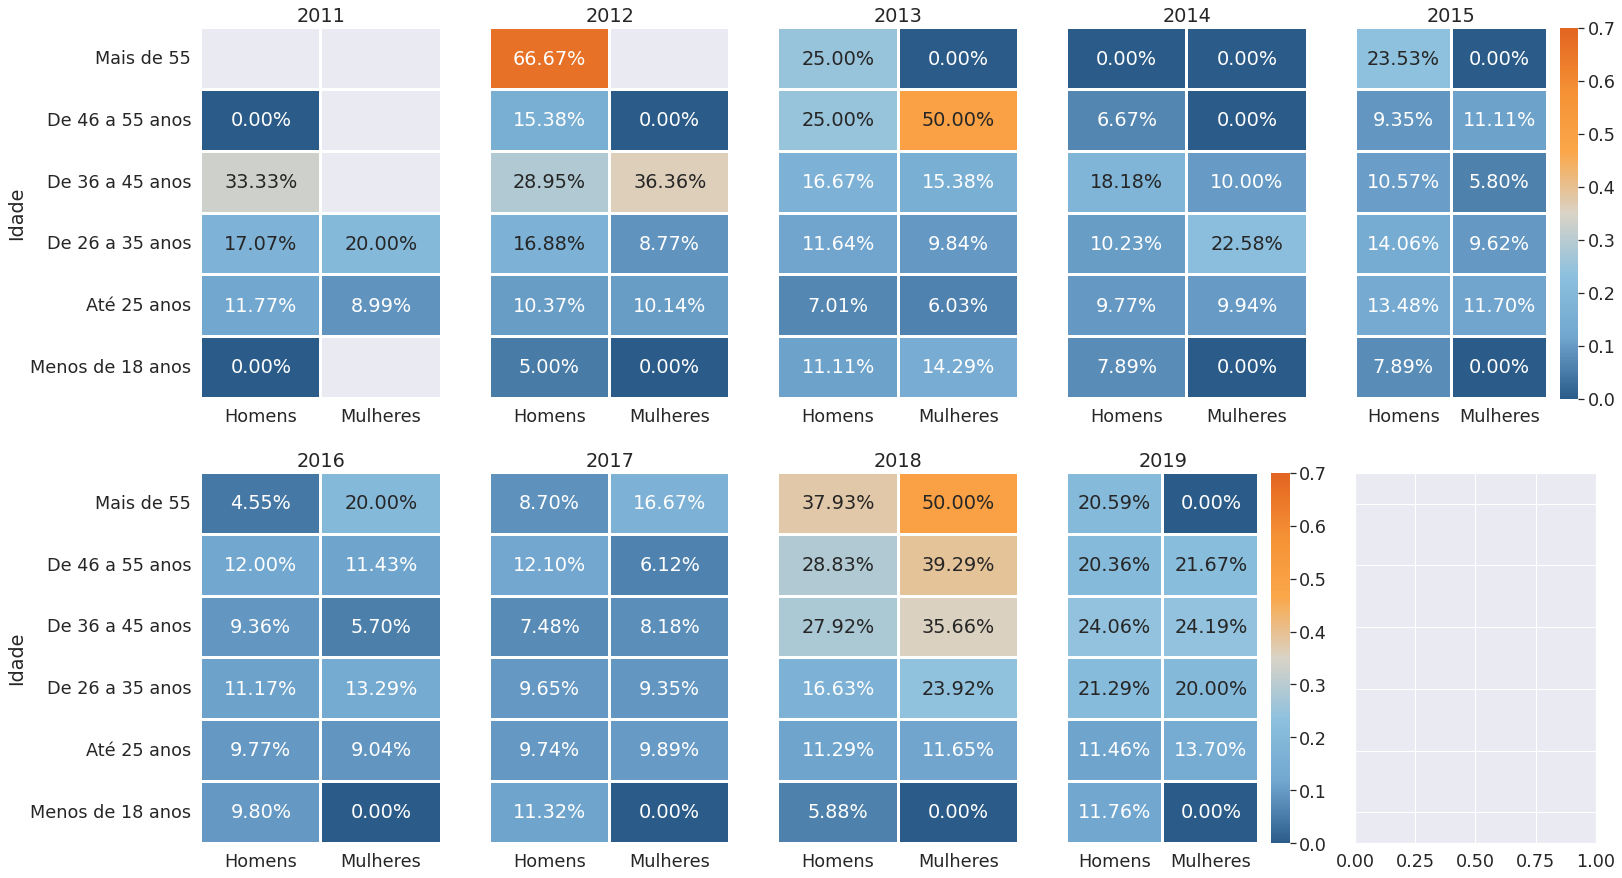
\includegraphics[width=1\textwidth]{Figuras/calorIdade.png}
\caption{Evasão do conjunto de projetos selecionados por ano e faixa etária}
\label{fig:calorIdade}
\end{figure}

As Tabelas \ref{tab:numabsoluto2011Idade}, \ref{tab:numabsoluto2014Idade} e \ref{tab:numabsoluto2017Idade} apresentam os valores absolutos de estudante dos anos de 2011 a 2019 por faixa etária.

\begin{table}[H]
\caption{Número absoluto de estudantes por ano, gênero e idade de 2011 a 2013}
\label{tab:numabsoluto2011Idade}
\resizebox{\textwidth}{!}{%
\begin{tabular}{c|cc|cc|cc|}
\cline{2-7}
                                                                        & \multicolumn{2}{c|}{\cellcolor[HTML]{C0C0C0}\textbf{2011}}                                               & \multicolumn{2}{c|}{\cellcolor[HTML]{C0C0C0}\textbf{2012}}                                               & \multicolumn{2}{c|}{\cellcolor[HTML]{C0C0C0}\textbf{2013}}                                               \\ \cline{2-7} 
\multirow{-2}{*}{}                                                      & \multicolumn{1}{c|}{\cellcolor[HTML]{C0C0C0}\textbf{Homens}} & \cellcolor[HTML]{C0C0C0}\textbf{Mulheres} & \multicolumn{1}{c|}{\cellcolor[HTML]{C0C0C0}\textbf{Homens}} & \cellcolor[HTML]{C0C0C0}\textbf{Mulheres} & \multicolumn{1}{c|}{\cellcolor[HTML]{C0C0C0}\textbf{Homens}} & \cellcolor[HTML]{C0C0C0}\textbf{Mulheres} \\ \hline
\multicolumn{1}{|c|}{\cellcolor[HTML]{C0C0C0}\textbf{Mais de 55 anos}}  & \multicolumn{1}{c|}{0}                                       & 0                                         & \multicolumn{1}{c|}{3}                                       & 0                                         & \multicolumn{1}{c|}{2}                                       & 1                                         \\ \hline
\multicolumn{1}{|c|}{\cellcolor[HTML]{C0C0C0}\textbf{De 46 a 55 anos}}  & \multicolumn{1}{c|}{2}                                       & 0                                         & \multicolumn{1}{c|}{13}                                      & 2                                         & \multicolumn{1}{c|}{14}                                      & 2                                         \\ \hline
\multicolumn{1}{|c|}{\cellcolor[HTML]{C0C0C0}\textbf{De 36 a 45 anos}}  & \multicolumn{1}{c|}{6}                                       & 0                                         & \multicolumn{1}{c|}{36}                                      & 11                                        & \multicolumn{1}{c|}{35}                                      & 9                                         \\ \hline
\multicolumn{1}{|c|}{\cellcolor[HTML]{C0C0C0}\textbf{De 26 a 35 anos}}  & \multicolumn{1}{c|}{41}                                      & 5                                         & \multicolumn{1}{c|}{370}                                     & 55                                        & \multicolumn{1}{c|}{367}                                     & 50                                        \\ \hline
\multicolumn{1}{|c|}{\cellcolor[HTML]{C0C0C0}\textbf{De 18 a 25 anos}}  & \multicolumn{1}{c|}{603}                                     & 89                                        & \multicolumn{1}{c|}{1634}                                    & 274                                       & \multicolumn{1}{c|}{1732}                                    & 302                                       \\ \hline
\multicolumn{1}{|c|}{\cellcolor[HTML]{C0C0C0}\textbf{Menos de 18 anos}} & \multicolumn{1}{c|}{0}                                       & 0                                         & \multicolumn{1}{c|}{16}                                      & 3                                         & \multicolumn{1}{c|}{33}                                      & 7                                         \\ \hline
\end{tabular}%
}
\end{table}

\begin{table}[H]
\caption{Número absoluto de estudantes por ano, gênero e idade de 2014 a 2016}
\label{tab:numabsoluto2014Idade}
\resizebox{\textwidth}{!}{%
\begin{tabular}{c|cc|cc|cc|}
\cline{2-7}
                                                                        & \multicolumn{2}{c|}{\cellcolor[HTML]{C0C0C0}\textbf{2014}}                                               & \multicolumn{2}{c|}{\cellcolor[HTML]{C0C0C0}\textbf{2015}}                                               & \multicolumn{2}{c|}{\cellcolor[HTML]{C0C0C0}\textbf{2016}}                                               \\ \cline{2-7} 
\multirow{-2}{*}{}                                                      & \multicolumn{1}{c|}{\cellcolor[HTML]{C0C0C0}\textbf{Homens}} & \cellcolor[HTML]{C0C0C0}\textbf{Mulheres} & \multicolumn{1}{c|}{\cellcolor[HTML]{C0C0C0}\textbf{Homens}} & \cellcolor[HTML]{C0C0C0}\textbf{Mulheres} & \multicolumn{1}{c|}{\cellcolor[HTML]{C0C0C0}\textbf{Homens}} & \cellcolor[HTML]{C0C0C0}\textbf{Mulheres} \\ \hline
\multicolumn{1}{|c|}{\cellcolor[HTML]{C0C0C0}\textbf{Mais de 55 anos}}  & \multicolumn{1}{c|}{2}                                       & 1                                         & \multicolumn{1}{c|}{17}                                      & 3                                         & \multicolumn{1}{c|}{17}                                      & 4                                         \\ \hline
\multicolumn{1}{|c|}{\cellcolor[HTML]{C0C0C0}\textbf{De 46 a 55 anos}}  & \multicolumn{1}{c|}{10}                                      & 2                                         & \multicolumn{1}{c|}{106}                                     & 27                                        & \multicolumn{1}{c|}{107}                                     & 32                                        \\ \hline
\multicolumn{1}{|c|}{\cellcolor[HTML]{C0C0C0}\textbf{De 36 a 45 anos}}  & \multicolumn{1}{c|}{35}                                      & 8                                         & \multicolumn{1}{c|}{442}                                     & 137                                       & \multicolumn{1}{c|}{476}                                     & 145                                       \\ \hline
\multicolumn{1}{|c|}{\cellcolor[HTML]{C0C0C0}\textbf{De 26 a 35 anos}}  & \multicolumn{1}{c|}{409}                                     & 46                                        & \multicolumn{1}{c|}{2314}                                    & 533                                       & \multicolumn{1}{c|}{2346}                                    & 544                                       \\ \hline
\multicolumn{1}{|c|}{\cellcolor[HTML]{C0C0C0}\textbf{De 18 a 25 anos}}  & \multicolumn{1}{c|}{1836}                                    & 329                                       & \multicolumn{1}{c|}{5674}                                    & 1110                                      & \multicolumn{1}{c|}{5646}                                    & 1051                                      \\ \hline
\multicolumn{1}{|c|}{\cellcolor[HTML]{C0C0C0}\textbf{Menos de 18 anos}} & \multicolumn{1}{c|}{35}                                      & 3                                         & \multicolumn{1}{c|}{33}                                      & 2                                         & \multicolumn{1}{c|}{45}                                      & 10                                        \\ \hline
\end{tabular}%
}
\end{table}

\begin{table}[H]
\caption{Número absoluto de estudantes por ano, gênero e idade de 2017 a 2019}
\label{tab:numabsoluto2017Idade}
\resizebox{\textwidth}{!}{%
\begin{tabular}{c|cc|cc|cc|}
\cline{2-7}
                                                                        & \multicolumn{2}{c|}{\cellcolor[HTML]{C0C0C0}\textbf{2017}}                                               & \multicolumn{2}{c|}{\cellcolor[HTML]{C0C0C0}\textbf{2018}}                                               & \multicolumn{2}{c|}{\cellcolor[HTML]{C0C0C0}\textbf{2019}}                                               \\ \cline{2-7} 
\multirow{-2}{*}{}                                                      & \multicolumn{1}{c|}{\cellcolor[HTML]{C0C0C0}\textbf{Homens}} & \cellcolor[HTML]{C0C0C0}\textbf{Mulheres} & \multicolumn{1}{c|}{\cellcolor[HTML]{C0C0C0}\textbf{Homens}} & \cellcolor[HTML]{C0C0C0}\textbf{Mulheres} & \multicolumn{1}{c|}{\cellcolor[HTML]{C0C0C0}\textbf{Homens}} & \cellcolor[HTML]{C0C0C0}\textbf{Mulheres} \\ \hline
\multicolumn{1}{|c|}{\cellcolor[HTML]{C0C0C0}\textbf{Mais de 55 anos}}  & \multicolumn{1}{c|}{22}                                      & 5                                         & \multicolumn{1}{c|}{26}                                      & 5                                         & \multicolumn{1}{c|}{22}                                      & 2                                         \\ \hline
\multicolumn{1}{|c|}{\cellcolor[HTML]{C0C0C0}\textbf{De 46 a 55 anos}}  & \multicolumn{1}{c|}{139}                                     & 44                                        & \multicolumn{1}{c|}{138}                                     & 50                                        & \multicolumn{1}{c|}{107}                                     & 36                                        \\ \hline
\multicolumn{1}{|c|}{\cellcolor[HTML]{C0C0C0}\textbf{De 36 a 45 anos}}  & \multicolumn{1}{c|}{646}                                     & 209                                       & \multicolumn{1}{c|}{699}                                     & 211                                       & \multicolumn{1}{c|}{579}                                     & 156                                       \\ \hline
\multicolumn{1}{|c|}{\cellcolor[HTML]{C0C0C0}\textbf{De 26 a 35 anos}}  & \multicolumn{1}{c|}{2612}                                    & 600                                       & \multicolumn{1}{c|}{2579}                                    & 569                                       & \multicolumn{1}{c|}{2407}                                    & 454                                       \\ \hline
\multicolumn{1}{|c|}{\cellcolor[HTML]{C0C0C0}\textbf{De 18 a 25 anos}}  & \multicolumn{1}{c|}{5837}                                    & 1068                                      & \multicolumn{1}{c|}{5779}                                    & 989                                       & \multicolumn{1}{c|}{5502}                                    & 942                                       \\ \hline
\multicolumn{1}{|c|}{\cellcolor[HTML]{C0C0C0}\textbf{Menos de 18 anos}} & \multicolumn{1}{c|}{51}                                      & 11                                        & \multicolumn{1}{c|}{30}                                      & 9                                         & \multicolumn{1}{c|}{32}                                      & 4                                         \\ \hline
\end{tabular}%
}
\end{table}

Independente do ano observado a faixa etária que mais apresenta estudantes é de 18 a 25 anos, logo em seguida dos estudantes de 26 a 35 anos. A faixa etária que mais apresenta disparidade entre o número de estudantes por gênero é a de menores de 18 anos, onde o número de homens é  6,5 vezes maior que o número de mulheres em uma média de todos os anos, seguido da faixa etária de 26 a 35 anos, que o número de homens é em média 6 vezes maior que o número de mulheres, também considerando os anos de 2011 a 2019. A faixa etária que apresenta menor disparidade entre os gêneros é a faixa dos 36 a 45 anos, onde o número de homens é 3,79 vezes maior que o número de mulheres.

\subsection{Presença Feminina nos Projetos Selecionados}\label{sub:mulherHomemProjeto}

Com todas as divisões apresentadas nas análises anteriores, a Figura \ref{fig:homensMulheresCincoProjetos} apresenta o número de estudantes possivelmente afetados pelos 5 projetos, mostrando mais uma vez a grande desigualdade de gênero nos cursos de TIC, onde a onda representada pela cor laranja mostra-se muito maior do que a onda azul que representa homens e mulheres consecutivamente.

\begin{figure}[H]
\centering
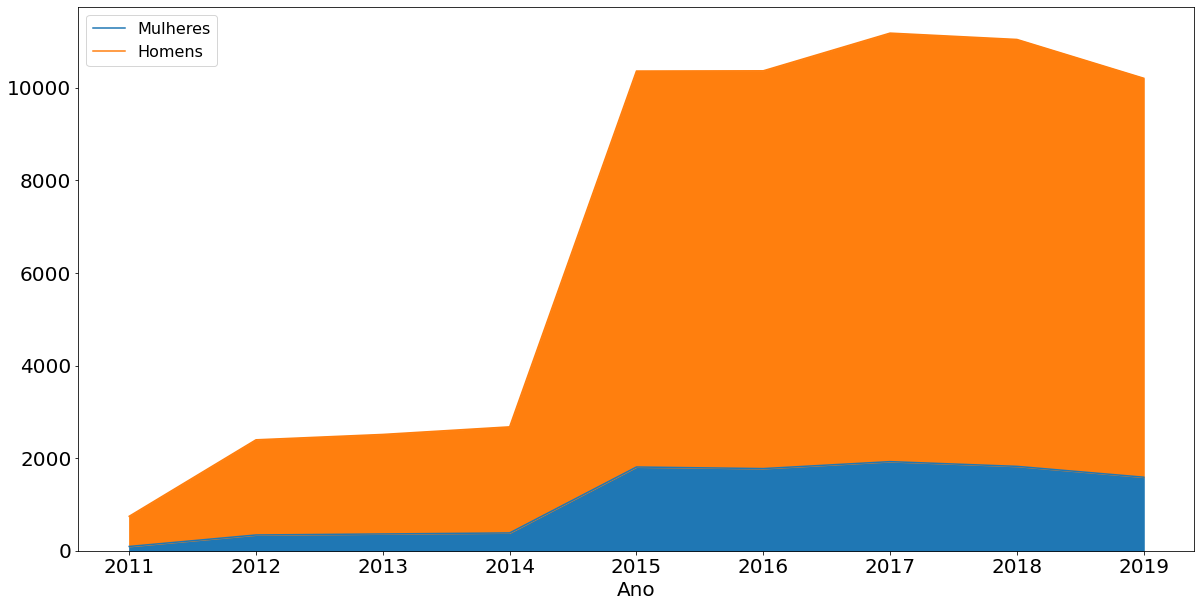
\includegraphics[width=1\textwidth]{Figuras/homensMulheresCincoProjetos.png}
\caption{Estudantes afetados por ano e gênero dos 5 projetos}
\label{fig:homensMulheresCincoProjetos}
\end{figure}

A Figura \ref{fig:homensMulheresCincoProjetos} considera o início do conjunto de projetos selecionados para contabilizar o número dos estudantes, por isso a alta no ano de 2015, onde dois projetos, WoMakersCode e Cunhantã Digital e Meninas Digitais Regional Mato Grosso, iniciaram.

\subsection{Participação em Atividade Extracurricular}\label{sub:extracurricular}

A Figura \ref{fig:extraCurricular} apresenta a participação dos estudantes em atividades extracurriculares. Apesar da nítida desigualdade, proporcionalmente de todos os homens 13,08\% fazem alguma atividade extracurricular, já as mulheres  13,43\% fazem alguma atividade. 

\begin{figure}[H]
\centering
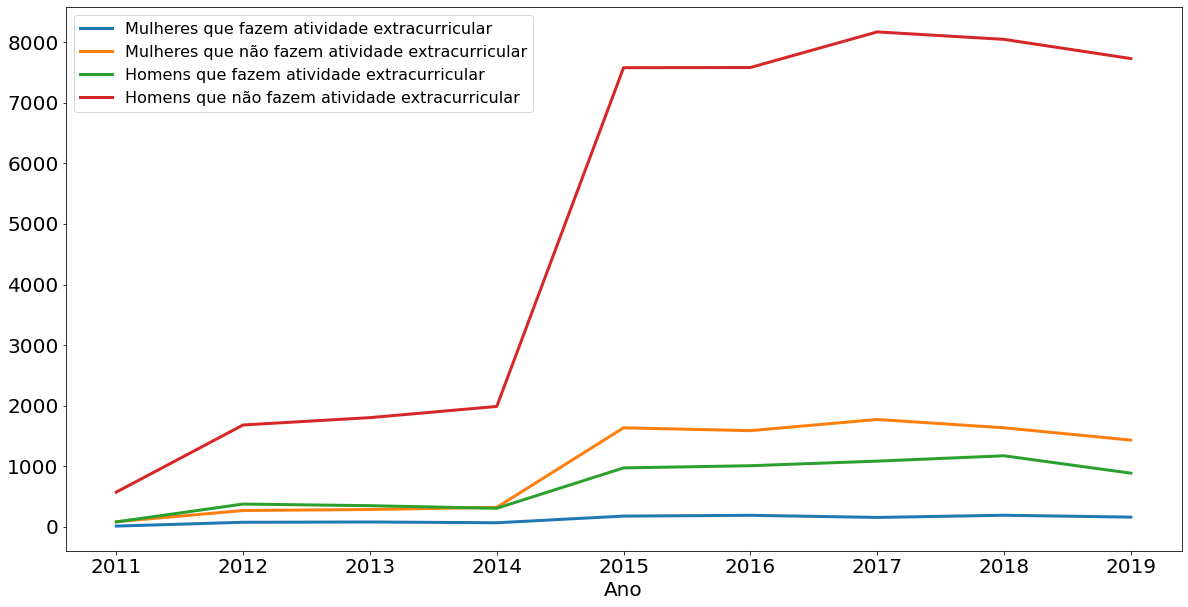
\includegraphics[width=1\textwidth]{Figuras/extraCurricular.png}
\caption{Participação em atividade extracurricular por gênero}
\label{fig:extraCurricular}
\end{figure}

A alta no ano de 2015, mais uma vez se dá pelo início dos projetos WoMakersCode e Cunhantã Digital. A Figura \ref{fig:extraCurricular} apresenta números absolutos de estudantes que participam ou não de atividade extracurricular no decorrer dos anos e como o número de homens é neste caso sempre superior ao número de mulheres, os homens também participam mais das atividades extracurriculares. 

% \subsection{Corpo Docente}\label{sub:docentes}

% Utilizando a mesma base do INEP e as IES de todas as análises anteriores, conforme o gráfico da Figura \ref{fig:professorGenero} a desigualdade de gênero também se apresenta no corpo docente.

% \begin{figure}[H]
% \centering
% 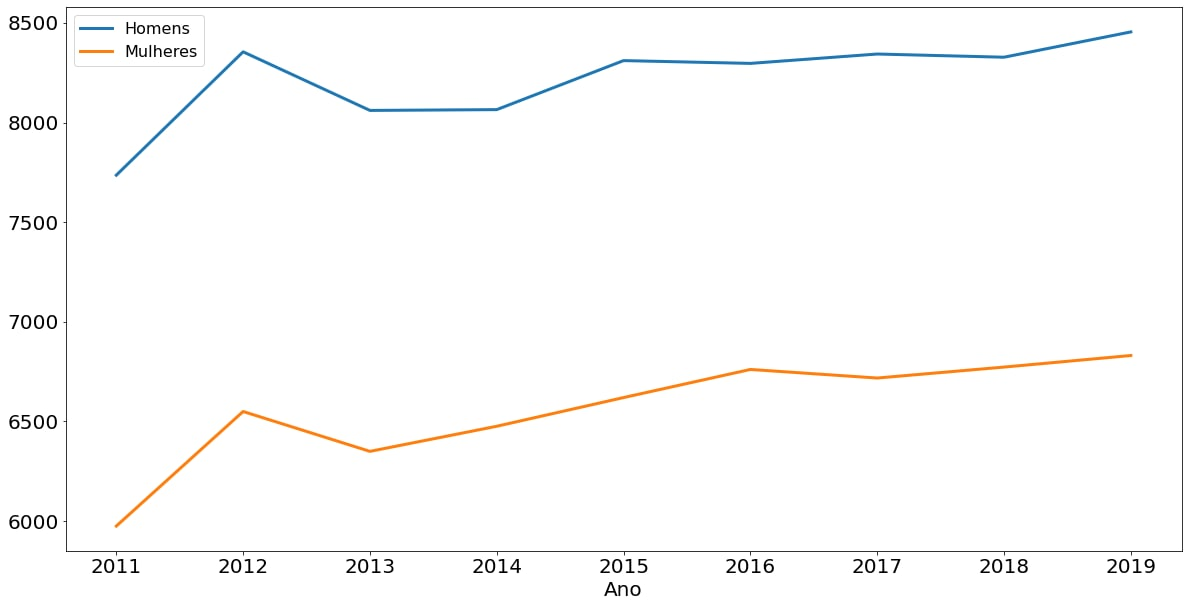
\includegraphics[width=1\textwidth]{Figuras/professores_sexo.jpeg}
% \caption{Participação em atividade extracurricular por gênero}
% \label{fig:professorGenero}
% \end{figure}

% Com a Figura \ref{fig:professorGenero} é de se estranhar o número alto de professores. Praticamente se igualando ao número dos alunos, porém as análises de corpo docente tornam-se dificultosas e limitadas por não existir a relação entre professor e curso, logo, as variáveis presentes na base do INEP sobre o corpo docente relacionam-se com a IES e não um curso específico.

% As variáveis presentes na base SUP\_DOCENTE do INEP são apenas variáveis da IES como código único de identificação da IES, tipo da categoria administrativa da IES e tipo da organização acadêmica da IES e variáveis do docente como escolaridade, gênero, regime de trabalho, data de nascimento e etc., não mencionando nada sobre curso. 


% %todas as análises sobre os projetos


\section{Entrevistas}\label{sec:Questionario}
%Questionário com foca na evasão.
%analises realizadas
Após todas as análises apresentadas na Seção \ref{sec:Avaliacoes} onde entende-se o panorama da presença de mulheres nos cursos de Computação e Tecnologias da Informação e Comunicação este trabalho também investigará por meio de entrevistas semi-estruturadas com pessoas dos projetos parceiros do Programa Meninas Digitais como estes projetos tem influenciado a presença e permanência de mulheres nos cursos de suas instituições.

O roteiro das entrevistas está sendo desenvolvido e terá perguntas para entender como o projeto interage com estudante, curso, instituição e corpo docente.

Este trabalho será submetido ao Comitê de Ética em breve. Todas as pessoas participantes deverão aceitar um Termo de Consentimento Livre e Esclarecido, apresentado no Apêndice \ref{ap:Termo}.

\section{Discussão do Capítulo}\label{sec:discussaoCapituloAnalises}
Neste capítulo foram apresentadas as análises sobre os dados do INEP do conjunto de projetos selecionados. As observações foram relacionadas aos estudantes, ano, gênero, idade, forma de ingresso e se eles participam ou não de atividades extracurriculares.

As análises apresentadas no capítulo podem ser continuadas em diversos outros gráficos e tabelas. Com isso pretende-se seguir e realizar novas análises, trazendo outras perspectivas e após as entrevistas, busca-se analisar a presença das mulheres nos cursos de TIC e a possível relação com as ações dos projetos parceiros do programa Meninas Digitais.
\chapter{Considerações}\label{cap:Consideracoes}
O principal objetivo deste trabalho está na análise da presença das mulheres nos cursos de TIC das universidades brasileiras e a busca por uma possível relação com as ações dos projetos parceiros do programa Meninas Digitais da SBC. 

Para encontrar esta possível relação inicialmente fez-se uma investigação e pesquisa exploratória sobre a evasão escolar e sua relação com gênero e uma exploração de ações realizadas para diminuir a evasão das mulheres na área das STEM.

Com a realização do Mapeamento Sistemática da Literatura, foi possível identificar e reformular o objetivo deste trabalho. Foi possível também trazer algumas informações importantes, como as definições de evasão e as principais variáveis consideradas para sua previsão.

Após todas as definições e investigações, fez-se a coleta de dados relacionados a evasão e gênero, tornando possível as análises. As análises envolvem características do estudante e para a próxima etapa de trabalho, pretende-se explorar melhor todas estas informações, trazendo também outras perspectivas ainda não abordadas.

Diante disso, o trabalho apresenta-se em construção. O cenário da presença feminina nos cursos de TIC foi explorado parcialmente e as entrevistas, assim que elaboradas, são promissoras para a efetiva busca do objetivo desta dissertação.


\section{Cronograma}\label{sec:Cronograma}
A fase atual da pesquisa é a elaboração e validação das perguntas da entrevista.

\begin{table}[h]
\centering
\caption{Cronograma de Atividades}
\label{tab:ProjetosMeninasDigitais}
\resizebox{\textwidth}{!}{%
\begin{tabular}{|l|l|l|l|l|l|l|}
\hline
Atividade                                          & 07/2022                  & 08/2022                  & 09/2022                                         & 10/2022                  & 11/2022                  & 12/2022                  \\ \hline
Validação das perguntas        & \cellcolor[HTML]{C0C0C0} &                          &                                                 &                          &                          &                          \\ \hline
Contato com selecionados                &                          & \cellcolor[HTML]{C0C0C0} &                                                 &                          &                          &                          \\ \hline
Aplicação da entrevista         &                          & \cellcolor[HTML]{C0C0C0} &                                                 &                          &                          &                          \\ \hline
Análises finais dos dados do INEP                 &                          &                          & \cellcolor[HTML]{C0C0C0}{\color[HTML]{000000} } &                          &                          &                          \\ \hline
Análise dos dados das entrevistas &                          &                          &                                                 & \cellcolor[HTML]{C0C0C0} &                          &                          \\
\hline
Triangulação dos dados                            &                          &                          &                                                 &                        \cellcolor[HTML]{C0C0C0}  & \cellcolor[HTML]{C0C0C0} &                          \\
\hline
Escrita da dissertação                            &                         \cellcolor[HTML]{C0C0C0} &                         \cellcolor[HTML]{C0C0C0} &                                                \cellcolor[HTML]{C0C0C0} &                        \cellcolor[HTML]{C0C0C0}  & \cellcolor[HTML]{C0C0C0} &                          \\ \hline
Defesa da dissertação                             &                          &                          &                                                 &                          &                          & \cellcolor[HTML]{C0C0C0} \\ \hline
\end{tabular}%
}
\end{table}

\section{Resultados Parciais}\label{sec:ResultadosParciais}
 Este projeto de pesquisa em desenvolvimento apresenta alguns resultados parciais como:
 As análises gráficas a partir dos dados do INEP foram organizadas em um site público e como fruto desta produção tem-se a publicação do artigo intitulado 'Ferramenta de Visualização de Dados do Censo da Educação Superior do INEP' que foi aceito para ser apresentado no Congresso da SBC de 2022 no 10º Workshop de Computação Aplicada em Governo Eletrônico. O MSL está em processo final de produção para submissão.

Além disso também foi produzido e submetido na Revista Novas Tecnologias na Educação o artigo intitulado 'Análise da evasão Feminina nos Cursos de Ciência da Computação das Universidades Públicas e Presenciais de Santa Catarina' que apresenta uma análise dos dados do INEP do ensino superior, com foco nos cursos de bacharelado em Ciência
da Computação nas universidades de ensino presencial e gratuito do estado de Santa Catarina, abrangendo os anos de 2015 a 2019. O trabalho tem como
objetivo apresentar as relações comparativas entre gênero, evasão e demais fatores impactantes como raça, forma de ingresso e idade. Como resultado, o artigo apresenta uma grande disparidade nas taxas, observando a maior evasão em ambos os gêneros acima de 35 anos.
%falar das producoes e artigos submetidos..

% -----------------------------------------------------------------
% ELEMENTOS PÓS-TEXTUAIS
% -----------------------------------------------------------------
\postextual

% Você pode comentar os elementos que não deseja em seu trabalho;

% Referências bibliográficas
\bibliography{abntex2-ref_UDESC_2020}	% Elemento Obrigatório

%% ----------------------------------------------------------
% Glossário
% ----------------------------------------------------------

%Consulte o manual da classe abntex2 para orientações sobre o glossário.

%\glossary




% ----------------------------------------------------------
% Glossário (Formatado Manualmente)
% ----------------------------------------------------------

\chapter*{GLOSSÁRIO}
\addcontentsline{toc}{chapter}{GLOSSÁRIO}

{ \setlength{\parindent}{0pt} % ambiente sem indentação

\textbf{Ardósia}: Rocha metamórfica sílico-argilosa formada pela transformação da argila sob pressão e temperatura, endurecida em finas lamelas.

\textbf{Arenito}: rocha sedimentária de origem detrítica formada de grãos agregados por um cimento natural silicoso, calcário ou ferruginoso que comunica ao conjunto em geral qualidades de dureza e compactação.

\textbf{Feldspato}: grupo de silicatos de sódio, potássio, cálcio ou outros elementos que compreende dois subgrupos, os feldspatos alcalinos e os plagioclásios.






} % fim ambiente sem indentação


				% Elemento Opcional

% ----------------------------------------------------------
% Apêndices
% ----------------------------------------------------------

% ---
% Inicia os apêndices
% ---
\begin{apendicesenv}

% Imprime uma página indicando o início dos apêndices
%\partapendices

% ----------------------------------------------------------
%\chapter{Artigo produzido sobre predição da evasão escolar} \label{ap:ArtigoPredicao}

% ----------------------------------------------------------

\chapter{TERMO DE CONSENTIMENTO LIVRE E ESCLARECIDO}\label{ap:Termo}

O(a) senhor(a) está sendo convidado a participar de uma pesquisa de mestrado intitulada ANÁLISE DA PRESENÇA DE MULHERES NOS CURSOS DE COMPUTAÇÃO E TECNOLOGIAS DA INFORMAÇÃO E COMUNICAÇÃO, que fará entrevista, tendo como objetivo de analisar a presença das mulheres nos cursos de Computação e Tecnologias da Informação e Comunicação em universidades brasileiras e sua possível relação com as ações dos projetos parceiros do programa Meninas Digitais. Esta pesquisa envolve ambientes virtuais como e-mails, ligações de áudio e vídeo e uso de aplicativos de chamadas \textit{(Google Meet, Zoom ou Teams)}. Não é obrigatório responder todas as perguntas.

Por isso, antes de responder às perguntas/participar das atividades disponibilizadas em ambiente não presencial ou virtual, será apresentado este Termo de Consentimento Livre e Esclarecido, para a sua anuência. Esse Termo de Consentimento será enviado por e-mail institucional e deverá ser assinado. 

As informações coletadas serão armazenadas no computador da pesquisadora principal em uma pasta sem acesso externo e com senha, somente ela terá acesso as entrevistas.

O(a) Senhor(a) não terá despesas e nem será remunerado(a) pela participação na pesquisa. Será utilizada ferramenta gratuita para as entrevistas. Os(as) participantes escolherão o melhor dia e horário para sua participação. 

Os riscos destes procedimentos serão mínimos. A entrevista está prevista para durar em torno de 30 minutos. Caso você se sinta cansado(a) podemos fazer pausas ou interromper a entrevista a qualquer momento. A sua identidade será preservada pois cada indivíduo será identificado por um número e somente as pesquisadoras terão acesso aos dados brutos.

Os benefícios e vantagens em participar deste estudo serão o cenário das possíveis relações entre a evasão ou permanência de mulheres nos cursos de TIC com o Programa Meninas Digitais.
As pessoas que estarão acompanhando os procedimentos da pesquisa serão as pesquisadoras estudante de mestrado Maria Teresa Silva Santos, professora responsável Isabela Gasparini e professora responsável Luciana Bolan Frigo.

O(a) senhor(a) poderá se retirar do estudo a qualquer momento, sem qualquer tipo de constrangimento.
Solicitamos a sua autorização para o uso de seus dados para a produção de artigos técnicos e científicos. A sua privacidade será mantida através da não-identificação do seu nome.
É importante que o (a) senhor(a) guarde em seus arquivos uma cópia deste documento eletrônico, para tanto, será encaminhado para seu e-mail.
\newline 
\newline 

NOME DO PESQUISADOR RESPONSÁVEL:  Maria Teresa Silva Santos

NÚMERO DO TELEFONE: 48998032709	

ENDEREÇO ELETRÔNICO: maria.santos2805@edu.udesc.br ou mariat95@gmail.com	

ASSINATURA DO PESQUISADOR: 
\newline 
\newline 

\newline 
\begin{center}
Comitê de Ética em Pesquisa Envolvendo Seres Humanos – CEPSH/UDESC
    TERMO DE CONSENTIMENTO
\end{center} 

Declaro que fui informado sobre todos os procedimentos da pesquisa e, que recebi de forma clara e objetiva todas as explicações pertinentes ao projeto e, que todos os dados a meu respeito serão sigilosos. Eu compreendo que neste estudo, as medições dos experimentos/procedimentos de tratamento serão feitas em mim, e que fui informado que posso me retirar do estudo a qualquer momento.
\newline 
\newline 
Nome por extenso: 
\newline 
Assinatura: 
\newline 
Local: 
\newline 
Data: 
\newline 
\newline 



\chapter{ARTIGOS SELECIONADOS PARA O MSL}\label{ap:tabelaApendiceMSL}

\begin{longtable}[c]{|r|l|}
\caption{Artigos selecionados para o MSL}
\label{tab:mapeamentoArtigos}\\
\hline
\rowcolor[HTML]{C0C0C0} 
\multicolumn{1}{|c|}{\cellcolor[HTML]{C0C0C0}\textbf{ID}} &
  \multicolumn{1}{p{14.5cm}|}{\cellcolor[HTML]{C0C0C0}\textbf{Referência}} \\ \hline
\endfirsthead
%
\multicolumn{2}{c}%
{{\bfseries Table \thetable\ continuação da página anterior}} \\
\hline
\rowcolor[HTML]{C0C0C0} 
\multicolumn{1}{|c|}{\cellcolor[HTML]{C0C0C0}\textbf{ID}} &
  \multicolumn{1}{p{14.5cm}|}{\cellcolor[HTML]{C0C0C0}\textbf{Referência}} \\ \hline
\endhead
%
\multicolumn{1}{|c|}{1} &
  \multicolumn{1}{p{14.5cm}|}{NDOU, Ndiatenda; AJOODHA; Ritesh; JADHAV, Ashwini. A Case Study to Enhance Student Support Initiatives Through Forecasting Student Success in Higher-Education. Johanesburgo: ASTES Journal, 2021. 6 v. (Advances in Science, Technology and Engineering Systems Journal, n. 230-241).} \\ \hline
2 &
  \multicolumn{1}{p{14.5cm}|}{AI, Dan; ZHANG, Tiancheng; YU, Ge; SHAO, Xinying. A Dropout Prediction Framework Combined with Ensemble Feature Selection. New York: Association for Computing Machinery, 2020. (ICIET 2020: Proceedings of the 2020 8th International Conference on Information and Education Technology, n. 179-185).} \\ \hline
3 &
  \multicolumn{1}{p{14.5cm}|}{CHEN, Min; WU, Lifa. A dropout prediction method based on time series model in MOOCs. United Kingdom: Journal of Physics Conference Series, 2020. (ICDPAM 2020).} \\ \hline
4 &
  \multicolumn{1}{p{14.5cm}|}{MRHAR, Khaoul; DOUIMI, Otmane; ABIK, Mounia. A Dropout Predictor System in MOOCs Based on Neural Networks. Poland: Journal of Automation, Mobile Robotics and Intelligent Systems, 2020. 14 v.} \\ \hline
5 &
  \multicolumn{1}{p{14.5cm}|}{QUEIROGA, Emanuel; LOPES, João; KAPPEL, Kristofer; AGUIAR, Marilton; ARAUJO, Ricardo; MUNOZ, Robert; VILLARROEL, Rodolfo; CECHINEL, Cristian. A Learning Analytics Approach to Identify Students at Risk of Dropout: A Case Study with a Technical Distance Education Course. Multidisciplinary Digital Publishing Institute (MDPI), 2020. (Applied Sciences).} \\ \hline
6 &
  \multicolumn{1}{p{14.5cm}|}{COBOS, Ruth; OLMOS, Lara. A Learning Analytics Tool for Predictive Modeling of Dropout and Certificate Acquisition on MOOCs for Professional Learning. Bangkok: IEEE International Conference on Industrial Engineering and Engineering Management (IEEM), 2018. (IEEM 2018, n. 1533-1537).} \\ \hline
7 &
  \multicolumn{1}{p{14.5cm}|}{AHMED, Sheikh Arif; BILLAH, Md. Aref; KHAN, Shahidul Islam. A Machine Learning Approach to Performance and Dropout prediction in Computer Science: Bangladesh Perspective. Kharagpur: 11th International Conference on Computing, Communication and Networking Technologies (ICCCNT), 2020. (ICCCNT 2020, n. 1-6).} \\ \hline
8 &
  \multicolumn{1}{p{14.5cm}|}{LOTTERING, Roderick; HANS, Robert; LALL, Manoj. A model for the identification of students at risk of dropout at a university of technology. Durban: International Conference on Artificial Intelligence, Big Data, Computing and Data Communication Systems (icABCD), 2020. (icABCD, n. 1-8).} \\ \hline
9 &
  \multicolumn{1}{p{14.5cm}|}{FERNÁNDEZ-GARCÍA, Antonio Jesús; PRECIADO, Juan Carlo; MELCHOR, Fran; RODRIGUEZ-ECHEVERRIA, Roberto; CONEJERO, José María; SÁNCHEZ-FIGUEROA, Fernando. A Real-Life Machine Learning Experience for Predicting University Dropout at Different Stages Using Academic Data. IEEE, 2021. 9 v. (IEEEAccess, n. 133076-133090).} \\ \hline
10 &
  \multicolumn{1}{p{14.5cm}|}{BECKER, Brett A.; MOONEY, Catherine; KUMAR, Amruth N.; RUSSELL, Sean. A Simple, Language-Independent Approach to Identifying Potentially At-Risk Introductory Programming Students. New York: Association for Computing Machinery, 2021. (ACE '21: Australasian Computing Education Conference, n. 168-175).} \\ \hline
11 &
  \multicolumn{1}{p{14.5cm}|}{HAIYANG, Liu; WANG, Zhihai; BENACHOUR, Phillip; TUBMAN, Philip. A Time Series Classification Method for Behaviour-Based Dropout Prediction. Mumbai: IEEE 18th International Conference on Advanced Learning Technologies (ICALT), 2018. (IEEE 18th International Conference on Advanced Learning Technologies, n. 191-195).} \\ \hline
12 &
  \multicolumn{1}{p{14.5cm}|}{LAUREANO, Lanie. Affinity Propagation SMOTE approach for Imbalanced dataset used in Predicting Student at Risk of Low Performance. Philippines: International Journal of Advanced Trends in Computer Science and Engineering, 2020. 9 v. (International Journal of Advanced Trends in Computer Science and Engineering, 5066-5070).} \\ \hline
13 &
  \multicolumn{1}{p{14.5cm}|}{MANRIQUE, Rubén; NUNES, Bernardo Pereira; MARINO, Olga; CASANOVA, Marco Antonio; NURMIKKO-FULLER, Terhi. An Analysis of Student Representation, Representative Features and Classification Algorithms to Predict Degree Dropout. New York: Association for Computing Machinery, 2019. (Proceedings of the 9th International Conference on Learning Analytics \& Knowledge, n. 401-410).} \\ \hline
14 &
  \multicolumn{1}{p{14.5cm}|}{BAÑERES, David; RODRIGUEZ, M. Elena; GUERRERO-ROLDÁN, Ana Elena; KARADENIZ, Abdulkadir. An Early Warning System to Detect At-Risk Students in Online Higher Education. Multidisciplinary Digital Publishing Institute (MDPI), 2020. (Applied Sciences).} \\ \hline
15 &
  \multicolumn{1}{p{14.5cm}|}{PERIWAL, Nidhi; RANA, Keyur. An empirical comparison of models for dropout prophecy in MOOCs. Greater Noida: International Conference on Computing, Communication and Automation (ICCCA), 2017. (2017 International Conference on Computing, Communication and Automation (ICCCA) n. 906-911).} \\ \hline
16 &
  \multicolumn{1}{p{14.5cm}|}{DU, Xu; YANG, Juan; HUNG, Jui-Long. An integrated framework based on latent variational autoencoder for providing early warning of at-risk students. IEEE Access, v. 8, p. 10110-10122, 2020.} \\ \hline
17 &
  \multicolumn{1}{p{14.5cm}|}{QIU, Lin; LIU, Yanshen; LIU, Yi. An Integrated Framework With Feature Selection for Dropout Prediction in Massive Open Online Courses. IEEE Access. {[}S. l.{]}: Institute of Electrical and Electronics Engineers (IEEE), 2018. DOI 10.1109/access.2018.2881275. Disponível em: http://dx.doi.org/10.1109/ACCESS.2018.2881275.} \\ \hline
18 &
  \multicolumn{1}{p{14.5cm}|}{MARTINHO, Valquiria Ribeiro De Carvalho; NUNES, Clodoaldo; MINUSSI, Carlos Roberto. An Intelligent System for Prediction of School Dropout Risk Group in Higher Education Classroom Based on Artificial Neural Networks. 2013 IEEE 25th International Conference on Tools with Artificial Intelligence. {[}S. l.{]}: IEEE, nov. 2013. DOI 10.1109/ictai.2013.33. Disponível em: http://dx.doi.org/10.1109/ICTAI.2013.33.} \\ \hline
19 &
  \multicolumn{1}{p{14.5cm}|}{EL-RADY, Alla Abd. An Ontological Model to Predict Dropout Students Using Machine Learning Techniques. 2020 3rd International Conference on Computer Applications \&amp; Information Security (ICCAIS). {[}S. l.{]}: IEEE, mar. 2020. DOI 10.1109/iccais48893.2020.9096743. Disponível em: http://dx.doi.org/10.1109/ICCAIS48893.2020.9096743.} \\ \hline
20 &
  \multicolumn{1}{p{14.5cm}|}{OPAZO, Diego; MORENO, Sebastián; ÁLVAREZ-MIRANDA, Eduardo; PEREIRA, Jordi. Analysis of First-Year University Student Dropout through Machine Learning Models: A Comparison between Universities. Mathematics. {[}S. l.{]}: MDPI AG, 15 out. 2021. DOI 10.3390/math9202599. Disponível em: http://dx.doi.org/10.3390/math9202599.} \\ \hline
21 &
  \multicolumn{1}{p{14.5cm}|}{TIMBAL, Maricel A. Analysis of Student-at-Risk of Dropping out (SARDO) Using Decision Tree: An Intelligent Predictive Model for Reduction. International Journal of Machine Learning and Computing. {[}S. l.{]}: EJournal Publishing, jun. 2019. DOI 10.18178/ijmlc.2019.9.3.798. Disponível em: http://dx.doi.org/10.18178/ijmlc.2019.9.3.798.} \\ \hline
22 &
  \multicolumn{1}{p{14.5cm}|}{KANG, Kyehong; WANG, Sujing. Analyze and Predict Student Dropout from Online Programs. Proceedings of the 2nd International Conference on Compute and Data Analysis - ICCDA 2018. {[}S. l.{]}: ACM Press, 2018. DOI 10.1145/3193077.3193090. Disponível em: http://dx.doi.org/10.1145/3193077.3193090.} \\ \hline
23 &
  \multicolumn{1}{p{14.5cm}|}{PEREZ, Boris; CASTELLANOS, Camilo; CORREAL, Dario. Applying Data Mining Techniques to Predict Student Dropout: A Case Study. 2018 IEEE 1st Colombian Conference on Applications in Computational Intelligence (ColCACI). {[}S. l.{]}: IEEE, maio 2018. DOI 10.1109/colcaci.2018.8484847. Disponível em: http://dx.doi.org/10.1109/ColCACI.2018.8484847.} \\ \hline
24 &
  \multicolumn{1}{p{14.5cm}|}{LIANG, Jiajun; YANG, Jian; WU, Yongji; LI, Chao; ZHENG, Li. Big Data Application in Education: Dropout Prediction in Edx MOOCs. 2016 IEEE Second International Conference on Multimedia Big Data (BigMM). {[}S. l.{]}: IEEE, abr. 2016. DOI 10.1109/bigmm.2016.70. Disponível em: http://dx.doi.org/10.1109/BigMM.2016.70.} \\ \hline
25 &
  \multicolumn{1}{p{14.5cm}|}{MOGAVI, Reza Hadi; MA, Xiaojuan; HUI, Pan. Characterizing Student Engagement Moods for Dropout Prediction in Question Pool Websites. arXiv, 2021. DOI 10.48550/ARXIV.2102.00423. Disponível em: https://arxiv.org/abs/2102.00423.} \\ \hline
26 &
  \multicolumn{1}{p{14.5cm}|}{BEDREGAL-ALPACA, Norka; CORNEJO-APARICIO, Víctor; ZÁRATE-VALDERRAMA, Joshua; YANQUE-CHURO, Pedro. Classification Models for Determining Types of Academic Risk and Predicting Dropout in University Students. International Journal of Advanced Computer Science and Applications. {[}S. l.{]}: The Science and Information Organization, 2020. DOI 10.14569/ijacsa.2020.0110133. Disponível em: http://dx.doi.org/10.14569/IJACSA.2020.0110133.} \\ \hline
27 &
  \multicolumn{1}{p{14.5cm}|}{WU, Nannan; ZHANG, Lei; GAO, Yi; ZHANG, Mingfei; SUN, Xia; FENG, Jun. CLMS-Net. Proceedings of the ACM Turing Celebration Conference - China. {[}S. l.{]}: ACM, 17 maio 2019. DOI 10.1145/3321408.3322848. Disponível em: http://dx.doi.org/10.1145/3321408.3322848.} \\ \hline
28 &
  \multicolumn{1}{p{14.5cm}|}{SAGE, Andrew J.; CERVATO, Cinzia; GENSCHEL, Ulrike; OGILVIE, Craig A. Combining Academics and Social Engagement: A Major-Specific Early Alert Method to Counter Student Attrition in Science, Technology, Engineering, and Mathematics. Journal of College Student Retention: Research, Theory \&amp; Practice. {[}S. l.{]}: SAGE Publications, 11 jun. 2018. DOI 10.1177/1521025118780502. Disponível em: http://dx.doi.org/10.1177/1521025118780502.} \\ \hline
29 &
  \multicolumn{1}{p{14.5cm}|}{WEN, Yimin; TIAN, Ye; WEN, Boxi; ZHOU, Qing; CAI, Guoyong; LIU, Shaozhong. Consideration of the local correlation of learning behaviors to predict dropouts from MOOCs. Tsinghua Science and Technology. {[}S. l.{]}: Tsinghua University Press, jun. 2020. DOI 10.26599/tst.2019.9010013. Disponível em: http://dx.doi.org/10.26599/TST.2019.9010013.} \\ \hline
30 &
  \multicolumn{1}{p{14.5cm}|}{LIAO, Jinzhi; TANG, Jiuyang; ZHAO, Xiang. Course drop-out prediction on MOOC platform via clustering and tensor completion. Tsinghua Science and Technology. {[}S. l.{]}: Tsinghua University Press, ago. 2019. DOI 10.26599/tst.2018.9010110. Disponível em: http://dx.doi.org/10.26599/TST.2018.9010110.} \\ \hline
31 &
  \multicolumn{1}{p{14.5cm}|}{SUPIC, Haris; DONKO, Dzenana. Course-Specific Model for Prediction of At-Risk Students Based on Case-Based Reasoning. 2020 IEEE Integrated STEM Education Conference (ISEC). {[}S. l.{]}: IEEE, 1 ago. 2020. DOI 10.1109/isec49744.2020.9280572. Disponível em: http://dx.doi.org/10.1109/ISEC49744.2020.9280572.} \\ \hline
32 &
  \multicolumn{1}{p{14.5cm}|}{LIN, Shieu-Hong. Data mining for student retention management. 2012. (J. Comput. Sci. Coll. 27, 92–99).} \\ \hline
33 &
  \multicolumn{1}{p{14.5cm}|}{ROVIRA, Sergi; PUERTAS, Eloi; IGUAL, Laura. Data-driven system to predict academic grades and dropout. (J. Alberto Conejero, org.). PLOS ONE. {[}S. l.{]}: Public Library of Science (PLoS), 14 fev. 2017. DOI 10.1371/journal.pone.0171207. Disponível em: http://dx.doi.org/10.1371/journal.pone.0171207.} \\ \hline
34 &
  \multicolumn{1}{p{14.5cm}|}{SUN, Di; MAO, Yueheng; DU, Junlei; XU, Pengfei; ZHENG, Qinhua; SUN, Hongtao. Deep Learning for Dropout Prediction in MOOCs. 2019 Eighth International Conference on Educational Innovation through Technology (EITT). {[}S. l.{]}: IEEE, out. 2019. DOI 10.1109/eitt.2019.00025. Disponível em: http://dx.doi.org/10.1109/EITT.2019.00025.} \\ \hline
35 &
  \multicolumn{1}{p{14.5cm}|}{ULIYAN, Diaa; ALJALOUD, Abdulaziz Salamah; ALKHALIL, Adel; AMER, Hanan Salem Al; MOHAMED, Magdy Abd Elrhman Abdallah; ALOGALI, Azizah Fhad Mohammed. Deep Learning Model to Predict Students Retention Using BLSTM and CRF. IEEE Access. {[}S. l.{]}: Institute of Electrical and Electronics Engineers (IEEE), 2021. DOI 10.1109/access.2021.3117117. Disponível em: http://dx.doi.org/10.1109/ACCESS.2021.3117117.} \\ \hline
36 &
  \multicolumn{1}{p{14.5cm}|}{WANG, Wei; YU, Han; MIAO, Chunyan. Deep Model for Dropout Prediction in MOOCs. Proceedings of the 2nd International Conference on Crowd Science and Engineering - ICCSE’17. {[}S. l.{]}: ACM Press, 2017. DOI 10.1145/3126973.3126990. Disponível em: http://dx.doi.org/10.1145/3126973.3126990.} \\ \hline
37 &
  \multicolumn{1}{p{14.5cm}|}{MUTROFIN, Siti; KHALIMI, Abdul Muiz; KURNIAWAN, Eddy; GINARDI, Raden Venantius Hari; FATICHAH, Chastine; SARI, Yuita Arum. Detection of Potentially Students Drop Out of College in Case of Missing Value Using C4.5. 2019 International Conference on Sustainable Engineering and Creative Computing (ICSECC). {[}S. l.{]}: IEEE, ago. 2019. DOI 10.1109/icsecc.2019.8907014. Disponível em: http://dx.doi.org/10.1109/ICSECC.2019.8907014.} \\ \hline
38 &
  \multicolumn{1}{p{14.5cm}|}{KRYSHKO, Olena; FLEISCHER, Jens; WALDEYER, Julia; WIRTH, Joachim; LEUTNER, Detlev. Do motivational regulation strategies contribute to university students’ academic success? Learning and Individual Differences. {[}S. l.{]}: Elsevier BV, ago. 2020. DOI 10.1016/j.lindif.2020.101912. Disponível em: http://dx.doi.org/10.1016/j.lindif.2020.101912.} \\ \hline
39 &
  \multicolumn{1}{p{14.5cm}|}{SANI, Nor Samsiah; FIKRI, Ahmad; ALI, Zulaiha; ZAKREE, Mohd; NADIYAH, Khairul. Drop-Out Prediction in Higher Education Among B40 Students. International Journal of Advanced Computer Science and Applications. {[}S. l.{]}: The Science and Information Organization, 2020. DOI 10.14569/ijacsa.2020.0111169. Disponível em: http://dx.doi.org/10.14569/IJACSA.2020.0111169.} \\ \hline
40 &
  \multicolumn{1}{p{14.5cm}|}{LI, Wentao; GAO, Min; LI, Hua; XIONG, Qingyu; WEN, Junhao; WU, Zhongfu. Dropout prediction in MOOCs using behavior features and multi-view semi-supervised learning. 2016 International Joint Conference on Neural Networks (IJCNN). {[}S. l.{]}: IEEE, jul. 2016. DOI 10.1109/ijcnn.2016.7727598. Disponível em: http://dx.doi.org/10.1109/IJCNN.2016.7727598.} \\ \hline
41 &
  \multicolumn{1}{p{14.5cm}|}{LIMSATHITWONG, Kittinan; TIWATTHANONT, Kanda; YATSUNGNOEN, Tanasin. Dropout prediction system to reduce discontinue study rate of information technology students. 2018 5th International Conference on Business and Industrial Research (ICBIR). {[}S. l.{]}: IEEE, maio 2018. DOI 10.1109/icbir.2018.8391176. Disponível em: http://dx.doi.org/10.1109/ICBIR.2018.8391176.} \\ \hline
42 &
  \multicolumn{1}{p{14.5cm}|}{NUANKAEW, Pratya. Dropout Situation of Business Computer Students, University of Phayao. International Journal of Emerging Technologies in Learning (iJET). {[}S. l.{]}: International Association of Online Engineering (IAOE), 7 out. 2019. DOI 10.3991/ijet.v14i19.11177. Disponível em: http://dx.doi.org/10.3991/ijet.v14i19.11177.} \\ \hline
43 &
  \multicolumn{1}{p{14.5cm}|}{CHEN, Yuanzhe; CHEN, Qing; MINGQIAN ZHAO; BOYER, Sebastien; VEERAMACHANENI, Kalyan; QU, Huamin. DropoutSeer: Visualizing learning patterns in Massive Open Online Courses for dropout reasoning and prediction. 2016 IEEE Conference on Visual Analytics Science and Technology (VAST). {[}S. l.{]}: IEEE, out. 2016. DOI 10.1109/vast.2016.7883517. Disponível em: http://dx.doi.org/10.1109/VAST.2016.7883517.} \\ \hline
44 &
  \multicolumn{1}{p{14.5cm}|}{BEHR, Andreas; GIESE, Marco; TEGUIM K., Hervé D.; THEUNE, Katja. Dropping out from Higher Education in Germany an Empirical Evaluation of Determinants for Bachelor Students. Open Education Studies. {[}S. l.{]}: Walter de Gruyter GmbH, 8 set. 2020. DOI 10.1515/edu-2020-0104. Disponível em: http://dx.doi.org/10.1515/edu-2020-0104.} \\ \hline
45 &
  \multicolumn{1}{p{14.5cm}|}{XU, Yang; WILSON, Kevin. Early Alert Systems During a Pandemic: A Simulation Study on the Impact of Concept Drift. LAK21: 11th International Learning Analytics and Knowledge Conference. {[}S. l.{]}: ACM, 12 abr. 2021. DOI 10.1145/3448139.3448190. Disponível em: http://dx.doi.org/10.1145/3448139.3448190.} \\ \hline
46 &
  \multicolumn{1}{p{14.5cm}|}{KOSTOPOULOS, Georgios; KOTSIANTIS, Sotiris; RAGOS, Omiros; GRAPSA, Theodoula N. Early dropout prediction in distance higher education using active learning. 2017 8th International Conference on Information, Intelligence, Systems \&amp; Applications (IISA). {[}S. l.{]}: IEEE, ago. 2017. DOI 10.1109/iisa.2017.8316424. Disponível em: http://dx.doi.org/10.1109/IISA.2017.8316424.} \\ \hline
47 &
  \multicolumn{1}{p{14.5cm}|}{PANAGIOTAKOPOULOS, Theodor; KOTSIANTIS, Sotiris; KOSTOPOULOS, Georgios; IATRELLIS, Omiros; KAMEAS, Achilles. Early Dropout Prediction in MOOCs through Supervised Learning and Hyperparameter Optimization. Electronics. {[}S. l.{]}: MDPI AG, 16 jul. 2021. DOI 10.3390/electronics10141701. Disponível em: http://dx.doi.org/10.3390/electronics10141701.} \\ \hline
48 &
  \multicolumn{1}{p{14.5cm}|}{JAMJOOM, Mona; ALABDULKREEM, Eatedal; HADJOUNI, Myriam; KARIM, Faten; QARH, Maha. Early Prediction for At-Risk Students in an Introductory Programming Course Based on Student Self-Efficacy. Informatica. {[}S. l.{]}: Slovenian Association Informatika, 30 ago. 2021. DOI 10.31449/inf.v45i6.3528. Disponível em: http://dx.doi.org/10.31449/inf.v45i6.3528.} \\ \hline
49 &
  \multicolumn{1}{p{14.5cm}|}{MARTINS, Luiz Carlos Barbosa; CARVALHO, Rommel N.; CARVALHO, Ricardo S.; VICTORINO, Marcio C.; HOLANDA, Maristela. Early Prediction of College Attrition Using Data Mining. 2017 16th IEEE International Conference on Machine Learning and Applications (ICMLA). {[}S. l.{]}: IEEE, dez. 2017. DOI 10.1109/icmla.2017.000-6. Disponível em: http://dx.doi.org/10.1109/ICMLA.2017.000-6.} \\ \hline
50 &
  \multicolumn{1}{p{14.5cm}|}{AGUIAR, Everaldo; CHAWLA, Nitesh V.; BROCKMAN, Jay; AMBROSE, G. Alex; GOODRICH, Victoria. Engagement vs performance. Proceedings of the Fourth International Conference on Learning Analytics And Knowledge. {[}S. l.{]}: ACM, 24 mar. 2014. DOI 10.1145/2567574.2567583. Disponível em: http://dx.doi.org/10.1145/2567574.2567583.} \\ \hline
51 &
  \multicolumn{1}{p{14.5cm}|}{DA SILVA, Paulo M.; LIMA, Marilia N. C. A.; SOARES, Wedson L.; SILVA, Iago R. R.; DE A. FAGUNDES, Roberta A.; DE SOUZA, Fernado F. Ensemble Regression Models Applied to Dropout in Higher Education. 2019 8th Brazilian Conference on Intelligent Systems (BRACIS). {[}S. l.{]}: IEEE, out. 2019. DOI 10.1109/bracis.2019.00030. Disponível em: http://dx.doi.org/10.1109/BRACIS.2019.00030.} \\ \hline
52 &
  \multicolumn{1}{p{14.5cm}|}{KOSTOPOULOS, Georgios; KOTSIANTIS, Sotiris; PINTELAS, Panagiotis. Estimating student dropout in distance higher education using semi-supervised techniques. Proceedings of the 19th Panhellenic Conference on Informatics. {[}S. l.{]}: ACM, out. 2015. DOI 10.1145/2801948.2802013. Disponível em: http://dx.doi.org/10.1145/2801948.2802013.} \\ \hline
53 &
  \multicolumn{1}{p{14.5cm}|}{SILVA, Fernanda Cristina da; CABRAL, Thiago Luiz de Oliveira; PACHECO, Andressa Sasaki Vasques. Evasão ou permanência? Modelos preditivos para a gestão do Ensino Superior. Education Policy Analysis Archives. {[}S. l.{]}: Mary Lou Fulton Teacher College, 19 out. 2020. DOI 10.14507/epaa.28.5387. Disponível em: http://dx.doi.org/10.14507/epaa.28.5387.} \\ \hline
54 &
  \multicolumn{1}{p{14.5cm}|}{SANTOS, G.A.S.; BELLOZE, K.T.; TARRATACA, L.; HADDAD, D.B.; BORDIGNON, A.L.; BRANDAO, D.N. EvolveDTree: Analyzing Student Dropout in Universities. 2020 International Conference on Systems, Signals and Image Processing (IWSSIP). {[}S. l.{]}: IEEE, jul. 2020. DOI 10.1109/iwssip48289.2020.9145203. Disponível em: http://dx.doi.org/10.1109/IWSSIP48289.2020.9145203.} \\ \hline
55 &
  \multicolumn{1}{p{14.5cm}|}{HASBUN, Tomas; ARAYA, Alexandra; VILLALON, Jorge. Extracurricular Activities as Dropout Prediction Factors in Higher Education Using Decision Trees. 2016 IEEE 16th International Conference on Advanced Learning Technologies (ICALT). {[}S. l.{]}: IEEE, jul. 2016. DOI 10.1109/icalt.2016.66. Disponível em: http://dx.doi.org/10.1109/ICALT.2016.66.} \\ \hline
56 &
  \multicolumn{1}{p{14.5cm}|}{MAYRA, Alban; MAURICIO, David. Factors to predict dropout at the universities: A case of study in Ecuador. 2018 IEEE Global Engineering Education Conference (EDUCON). {[}S. l.{]}: IEEE, abr. 2018. DOI 10.1109/educon.2018.8363371. Disponível em: http://dx.doi.org/10.1109/EDUCON.2018.8363371.} \\ \hline
57 &
  \multicolumn{1}{p{14.5cm}|}{KORI, Kulli; PEDASTE, Margus; TONISSON, Eno; PALTS, Tauno; ALTIN, Heilo; RANTSUS, Ramon; SELL, Raivo; MURTAZIN, Kristina; RUUTMANN, Tiia. First-year dropout in ICT studies. 2015 IEEE Global Engineering Education Conference (EDUCON). {[}S. l.{]}: IEEE, mar. 2015. DOI 10.1109/educon.2015.7096008. Disponível em: http://dx.doi.org/10.1109/EDUCON.2015.7096008.} \\ \hline
58 &
  \multicolumn{1}{p{14.5cm}|}{AJOODHA, Ritesh; JADHAV, Ashwini; DUKHAN, Shalini. Forecasting Learner Attrition for Student Success at a South African University. Conference of the South African Institute of Computer Scientists and Information Technologists 2020. {[}S. l.{]}: ACM, 11 set. 2020. DOI 10.1145/3410886.3410973. Disponível em: http://dx.doi.org/10.1145/3410886.3410973.} \\ \hline
59 &
  \multicolumn{1}{p{14.5cm}|}{BERNARDO, Ana; CERVERO, Antonio; ESTEBAN, María; TUERO, Ellian; CASANOVA, Joana R.; ALMEIDA, Leandro S. Freshmen Program Withdrawal: Types and Recommendations. Frontiers in Psychology. {[}S. l.{]}: Frontiers Media SA, 21 set. 2017. DOI 10.3389/fpsyg.2017.01544. Disponível em: http://dx.doi.org/10.3389/fpsyg.2017.01544.} \\ \hline
60 &
  \multicolumn{1}{p{14.5cm}|}{ORTIGOSA, Alvaro; CARRO, Rosa M.; BRAVO-AGAPITO, Javier; LIZCANO, David; ALCOLEA, Juan Jesus; BLANCO, Oscar. From Lab to Production: Lessons Learnt and Real-Life Challenges of an Early Student-Dropout Prevention System. IEEE Transactions on Learning Technologies. {[}S. l.{]}: Institute of Electrical and Electronics Engineers (IEEE), 1 abr. 2019. DOI 10.1109/tlt.2019.2911608. Disponível em: http://dx.doi.org/10.1109/TLT.2019.2911608.} \\ \hline
61 &
  \multicolumn{1}{p{14.5cm}|}{QUEIROGA, Emanuel Marques; CECHINEL, Cristian; MATSUMURA ARAUJO, Ricardo; DA COSTA BRETANHA, Guilherme. Generating models to predict at-risk students in technical e-learning courses. 2016 XI Latin American Conference on Learning Objects and Technology (LACLO). {[}S. l.{]}: IEEE, out. 2016. DOI 10.1109/laclo.2016.7751770. Disponível em: http://dx.doi.org/10.1109/LACLO.2016.7751770.} \\ \hline
62 &
  \multicolumn{1}{p{14.5cm}|}{VAN HEESCH, M. M. J.; BOSMA, H.; TRAAG, T.; OTTEN, F. Hospital admissions and school dropout: a retrospective cohort study of the “selection hypothesis”. The European Journal of Public Health. {[}S. l.{]}: Oxford University Press (OUP), 10 set. 2011. DOI 10.1093/eurpub/ckr129. Disponível em: http://dx.doi.org/10.1093/eurpub/ckr129.} \\ \hline
63 &
  \multicolumn{1}{p{14.5cm}|}{HORI, Gen. Identifying Factors Contributing to University Dropout with Sparse Logistic Regression. 2018 7th International Congress on Advanced Applied Informatics (IIAI-AAI). {[}S. l.{]}: IEEE, jul. 2018. DOI 10.1109/iiai-aai.2018.00091. Disponível em: http://dx.doi.org/10.1109/IIAI-AAI.2018.00091.} \\ \hline
64 &
  \multicolumn{1}{p{14.5cm}|}{NOURI, Jalal; LARSSON, Ken; SAQR, Mohammed. Identifying Factors for Master Thesis Completion and Non-completion Through Learning Analytics and Machine Learning. Lecture Notes in Computer Science. {[}S. l.{]}: Springer International Publishing, 2019. DOI 10.1007/978-3-030-29736-7\_3. Disponível em: http://dx.doi.org/10.1007/978-3-030-29736-7\_3.} \\ \hline
65 &
  \multicolumn{1}{p{14.5cm}|}{UTARI, Meylani; WARSITO, Budi; KUSUMANINGRUM, Retno. Implementation of Data Mining for Drop-Out Prediction using Random Forest Method. 2020 8th International Conference on Information and Communication Technology (ICoICT). {[}S. l.{]}: IEEE, jun. 2020. DOI 10.1109/icoict49345.2020.9166276. Disponível em: http://dx.doi.org/10.1109/ICoICT49345.2020.9166276.} \\ \hline
66 &
  \multicolumn{1}{p{14.5cm}|}{SAMANI, Tej; CANHOTO, Ana Isabel; YORUK, Esin. Improving the Retention and Progression of Learners Through Intelligent Systems for Diagnosing Metacognitive Competencies – A Case Study in UK Further Education. Advances in Intelligent Systems and Computing. {[}S. l.{]}: Springer International Publishing, 2021. DOI 10.1007/978-3-030-74009-2\_3. Disponível em: http://dx.doi.org/10.1007/978-3-030-74009-2\_3.} \\ \hline
67 &
  \multicolumn{1}{p{14.5cm}|}{CSALÓDI, Róbert; ABONYI, János. Integrated Survival Analysis and Frequent Pattern Mining for Course Failure-Based Prediction of Student Dropout. Mathematics. {[}S. l.{]}: MDPI AG, 24 fev. 2021. DOI 10.3390/math9050463. Disponível em: http://dx.doi.org/10.3390/math9050463.} \\ \hline
68 &
  \multicolumn{1}{p{14.5cm}|}{VILORIA, Amelec; PADILLA, Jholman Garcia; VARGAS-MERCADO, Carlos; HERNÁNDEZ-PALMA, Hugo; LLINAS, Nataly Orellano; DAVID, Monica Arrozola. Integration of Data Technology for Analyzing University Dropout. Procedia Computer Science. {[}S. l.{]}: Elsevier BV, 2019. DOI 10.1016/j.procs.2019.08.079. Disponível em: http://dx.doi.org/10.1016/j.procs.2019.08.079.} \\ \hline
69 &
  \multicolumn{1}{p{14.5cm}|}{BARANYI, Máté; NAGY, Marcell; MOLONTAY, Roland. Interpretable Deep Learning for University Dropout Prediction. Proceedings of the 21st Annual Conference on Information Technology Education. {[}S. l.{]}: ACM, 7 out. 2020. DOI 10.1145/3368308.3415382. Disponível em: http://dx.doi.org/10.1145/3368308.3415382.} \\ \hline
70 &
  \multicolumn{1}{p{14.5cm}|}{DE JESUS, Cindy G.; LEDDA, Mark Kristian C. Intervention Support Program for Students at Risk of Dropping Out Using Fuzzy Logic-Based Prescriptive Analytics. 2021 IEEE 17th International Colloquium on Signal Processing \&amp; Its Applications (CSPA). {[}S. l.{]}: IEEE, 5 mar. 2021. DOI 10.1109/cspa52141.2021.9377304. Disponível em: http://dx.doi.org/10.1109/CSPA52141.2021.9377304.} \\ \hline
71 &
  \multicolumn{1}{p{14.5cm}|}{FREITAS, Francisco A. da S.; VASCONCELOS, Francisco F. X.; PEIXOTO, Solon A.; HASSAN, Mohammad Mehedi; DEWAN, M. Ali Akber; ALBUQUERQUE, Victor Hugo C. de; FILHO, Pedro P. Rebouças. IoT System for School Dropout Prediction Using Machine Learning Techniques Based on Socioeconomic Data. Electronics. {[}S. l.{]}: MDPI AG, 1 out. 2020. DOI 10.3390/electronics9101613. Disponível em: http://dx.doi.org/10.3390/electronics9101613.} \\ \hline
72 &
  \multicolumn{1}{p{14.5cm}|}{PALACIOS, Carlos A.; REYES-SUÁREZ, José A.; BEARZOTTI, Lorena A.; LEIVA, Víctor; MARCHANT, Carolina. Knowledge Discovery for Higher Education Student Retention Based on Data Mining: Machine Learning Algorithms and Case Study in Chile. Entropy. {[}S. l.{]}: MDPI AG, 20 abr. 2021. DOI 10.3390/e23040485. Disponível em: http://dx.doi.org/10.3390/e23040485.} \\ \hline
73 &
  \multicolumn{1}{p{14.5cm}|}{LIANG, Jiajun; LI, Chao; ZHENG, Li. Machine learning application in MOOCs: Dropout prediction. 2016 11th International Conference on Computer Science \&amp; Education (ICCSE). {[}S. l.{]}: IEEE, ago. 2016. DOI 10.1109/iccse.2016.7581554. Disponível em: http://dx.doi.org/10.1109/ICCSE.2016.7581554.} \\ \hline
74 &
  \multicolumn{1}{p{14.5cm}|}{SUKHBAATAR, Otgontsetseg; OGATA, Kohichi; USAGAWA, Tsuyoshi. Mining Educational Data to Predict Academic Dropouts: a Case Study in Blended Learning Course. TENCON 2018 - 2018 IEEE Region 10 Conference. {[}S. l.{]}: IEEE, out. 2018. DOI 10.1109/tencon.2018.8650138. Disponível em: http://dx.doi.org/10.1109/TENCON.2018.8650138.} \\ \hline
75 &
  \multicolumn{1}{p{14.5cm}|}{LI, Feifan; WEI, Zhengang. MOOC Dropout Prediction Based on Multi-view Learning. Journal of Physics: Conference Series. {[}S. l.{]}: IOP Publishing, 1 set. 2021. DOI 10.1088/1742-6596/2010/1/012120. Disponível em: http://dx.doi.org/10.1088/1742-6596/2010/1/012120.} \\ \hline
76 &
  \multicolumn{1}{p{14.5cm}|}{ZHENG, Yafeng; GAO, Zhanghao; WANG, Yihang; FU, Qian. MOOC Dropout Prediction Using FWTS-CNN Model Based on Fused Feature Weighting and Time Series. IEEE Access. {[}S. l.{]}: Institute of Electrical and Electronics Engineers (IEEE), 2020. DOI 10.1109/access.2020.3045157. Disponível em: http://dx.doi.org/10.1109/ACCESS.2020.3045157.} \\ \hline
77 &
  \multicolumn{1}{p{14.5cm}|}{WHITEHILL, Jacob; MOHAN, Kiran; SEATON, Daniel; ROSEN, Yigal; TINGLEY, Dustin. MOOC Dropout Prediction. Proceedings of the Fourth (2017) ACM Conference on Learning @ Scale. {[}S. l.{]}: ACM, 12 abr. 2017. DOI 10.1145/3051457.3053974. Disponível em: http://dx.doi.org/10.1145/3051457.3053974.} \\ \hline
78 &
  \multicolumn{1}{p{14.5cm}|}{NAGRECHA, Saurabh; DILLON, John Z.; CHAWLA, Nitesh V. MOOC Dropout Prediction. Proceedings of the 26th International Conference on World Wide Web Companion - WWW ’17 Companion. {[}S. l.{]}: ACM Press, 2017. DOI 10.1145/3041021.3054162. Disponível em: http://dx.doi.org/10.1145/3041021.3054162.} \\ \hline
79 &
  \multicolumn{1}{p{14.5cm}|}{CHEN, Yunfan; ZHANG, Ming. MOOC student dropout. Proceedings of the ACM Turing 50th Celebration Conference - China on - ACM TUR-C ’17. {[}S. l.{]}: ACM Press, 2017. DOI 10.1145/3063955.3063959. Disponível em: http://dx.doi.org/10.1145/3063955.3063959.} \\ \hline
80 &
  \multicolumn{1}{p{14.5cm}|}{ZHANG, Yan; CHANG, Liang; LIU, Tieyuan. MOOCs Dropout Prediction Based on Hybrid Deep Neural Network. 2020 International Conference on Cyber-Enabled Distributed Computing and Knowledge Discovery (CyberC). {[}S. l.{]}: IEEE, out. 2020. DOI 10.1109/cyberc49757.2020.00039. Disponível em: http://dx.doi.org/10.1109/CyberC49757.2020.00039.} \\ \hline
81 &
  \multicolumn{1}{p{14.5cm}|}{ZHOU, Ya; XU, Zhixiang. Multi-Model Stacking Ensemble Learning for Dropout Prediction in MOOCs. Journal of Physics: Conference Series. {[}S. l.{]}: IOP Publishing, 1 ago. 2020. DOI 10.1088/1742-6596/1607/1/012004. Disponível em: http://dx.doi.org/10.1088/1742-6596/1607/1/012004.} \\ \hline
82 &
  \multicolumn{1}{p{14.5cm}|}{ALBAN, Mayra; MAURICIO, David. Neural Networks to Predict Dropout at the Universities. International Journal of Machine Learning and Computing. {[}S. l.{]}: EJournal Publishing, abr. 2019. DOI 10.18178/ijmlc.2019.9.2.779. Disponível em: http://dx.doi.org/10.18178/ijmlc.2019.9.2.779.} \\ \hline
83 &
  \multicolumn{1}{p{14.5cm}|}{GOEL, Yamini; GOYAL, Rinkaj. On the Effectiveness of Self-Training in MOOC Dropout Prediction. Open Computer Science. {[}S. l.{]}: Walter de Gruyter GmbH, 22 jul. 2020. DOI 10.1515/comp-2020-0153. Disponível em: http://dx.doi.org/10.1515/comp-2020-0153.} \\ \hline
84 &
  \multicolumn{1}{p{14.5cm}|}{FURINI, Marco; GALLI, Giovanna; MARTINI, Maria Cristiana. On Using Video Lectures Data Usage to Predict University Students Dropout. Proceedings of the Conference on Information Technology for Social Good. {[}S. l.{]}: ACM, 9 set. 2021. DOI 10.1145/3462203.3475890. Disponível em: http://dx.doi.org/10.1145/3462203.3475890.} \\ \hline
85 &
  \multicolumn{1}{p{14.5cm}|}{PULIKOTTIL, Siby Charley; GUPTA, Manish. ONet – A Temporal Meta Embedding Network for MOOC Dropout Prediction. 2020 IEEE International Conference on Big Data (Big Data). {[}S. l.{]}: IEEE, 10 dez. 2020. DOI 10.1109/bigdata50022.2020.9378001. Disponível em: http://dx.doi.org/10.1109/BigData50022.2020.9378001.} \\ \hline
86 &
  \multicolumn{1}{p{14.5cm}|}{HE, Yanbai; CHEN, Rui; LI, Xinya; HAO, Chuanyan; LIU, Sijiang; ZHANG, Gangyao; JIANG, Bo. Online At-Risk Student Identification using RNN-GRU Joint Neural Networks. Information. {[}S. l.{]}: MDPI AG, 9 out. 2020. DOI 10.3390/info11100474. Disponível em: http://dx.doi.org/10.3390/info11100474.} \\ \hline
87 &
  \multicolumn{1}{p{14.5cm}|}{FONTANA, Luca; MASCI, Chiara; IEVA, Francesca; PAGANONI, Anna Maria. Performing Learning Analytics via Generalised Mixed-Effects Trees. Data. {[}S. l.{]}: MDPI AG, 9 jul. 2021. DOI 10.3390/data6070074. Disponível em: http://dx.doi.org/10.3390/data6070074.} \\ \hline
88 &
  \multicolumn{1}{p{14.5cm}|}{SOLIS, Martin; MOREIRA, Tania; GONZALEZ, Roberto; FERNANDEZ, Tatiana; HERNANDEZ, Maria. Perspectives to Predict Dropout in University Students with Machine Learning. 2018 IEEE International Work Conference on Bioinspired Intelligence (IWOBI). {[}S. l.{]}: IEEE, jul. 2018. DOI 10.1109/iwobi.2018.8464191. Disponível em: http://dx.doi.org/10.1109/IWOBI.2018.8464191.} \\ \hline
89 &
  \multicolumn{1}{p{14.5cm}|}{TSAI, Shuo-Chang; CHEN, Cheng-Huan; SHIAO, Yi-Tzone; CIOU, Jin-Shuei; WU, Trong-Neng. Precision education with statistical learning and deep learning: a case study in Taiwan. International Journal of Educational Technology in Higher Education. {[}S. l.{]}: Springer Science and Business Media LLC, 8 abr. 2020. DOI 10.1186/s41239-020-00186-2. Disponível em: http://dx.doi.org/10.1186/s41239-020-00186-2.} \\ \hline
90 &
  \multicolumn{1}{p{14.5cm}|}{BORRELLA, Inma; CABALLERO-CABALLERO, Sergio; PONCE-CUETO, Eva. Predict and Intervene. Proceedings of the Sixth (2019) ACM Conference on Learning @ Scale. {[}S. l.{]}: ACM, 24 jun. 2019. DOI 10.1145/3330430.3333634. Disponível em: http://dx.doi.org/10.1145/3330430.3333634.} \\ \hline
91 &
  \multicolumn{1}{p{14.5cm}|}{ADNAN, Muhammad; HABIB, Asad; ASHRAF, Jawad; MUSSADIQ, Shafaq; RAZA, Arsalan Ali; ABID, Muhammad; BASHIR, Maryam; KHAN, Sana Ullah. Predicting at-Risk Students at Different Percentages of Course Length for Early Intervention Using Machine Learning Models. IEEE Access. {[}S. l.{]}: Institute of Electrical and Electronics Engineers (IEEE), 2021. DOI 10.1109/access.2021.3049446. Disponível em: http://dx.doi.org/10.1109/ACCESS.2021.3049446.} \\ \hline
92 &
  \multicolumn{1}{p{14.5cm}|}{NAGY, Marcell; MOLONTAY, Roland. Predicting Dropout in Higher Education Based on Secondary School Performance. 2018 IEEE 22nd International Conference on Intelligent Engineering Systems (INES). {[}S. l.{]}: IEEE, jun. 2018. DOI 10.1109/ines.2018.8523888. Disponível em: http://dx.doi.org/10.1109/INES.2018.8523888.} \\ \hline
93 &
  \multicolumn{1}{p{14.5cm}|}{RADOVANOVIC, Sandro; DELIBASIC, Boris; SUKNOVIC, Milija. Predicting dropout in online learning environments. Computer Science and Information Systems. {[}S. l.{]}: National Library of Serbia, 2021. DOI 10.2298/csis200920053r. Disponível em: http://dx.doi.org/10.2298/CSIS200920053R.} \\ \hline
94 &
  \multicolumn{1}{p{14.5cm}|}{DEWAN, M. Ali Akber; LIN, Fuhua; WEN, Dunwei; KINSHUK. Predicting Dropout-Prone Students in E-Learning Education System. 2015 IEEE 12th Intl Conf on Ubiquitous Intelligence and Computing and 2015 IEEE 12th Intl Conf on Autonomic and Trusted Computing and 2015 IEEE 15th Intl Conf on Scalable Computing and Communications and Its Associated Workshops (UIC-ATC-ScalCom). {[}S. l.{]}: IEEE, ago. 2015. DOI 10.1109/uic-atc-scalcom-cbdcom-iop.2015.315. Disponível em: http://dx.doi.org/10.1109/UIC-ATC-ScalCom-CBDCom-IoP.2015.315.} \\ \hline
95 &
  \multicolumn{1}{p{14.5cm}|}{OROOJI, Marmar; CHEN, Jianhua. Predicting Louisiana Public High School Dropout through Imbalanced Learning Techniques. 2019 18th IEEE International Conference On Machine Learning And Applications (ICMLA). {[}S. l.{]}: IEEE, dez. 2019. DOI 10.1109/icmla.2019.00085. Disponível em: http://dx.doi.org/10.1109/ICMLA.2019.00085.} \\ \hline
96 &
  \multicolumn{1}{p{14.5cm}|}{KILIAN, Pascal; LOOSE, Frank; KELAVA, Augustin. Predicting Math Student Success in the Initial Phase of College With Sparse Information Using Approaches From Statistical Learning. Frontiers in Education. {[}S. l.{]}: Frontiers Media SA, 22 dez. 2020. DOI 10.3389/feduc.2020.502698. Disponível em: http://dx.doi.org/10.3389/feduc.2020.502698.} \\ \hline
97 &
  \multicolumn{1}{p{14.5cm}|}{WAN YAACOB, W F; MOHD SOBRI, N; NASIR, S A Md; WAN YAACOB, W F; NORSHAHIDI, N D; WAN HUSIN, W Z. Predicting Student Drop-Out in Higher Institution Using Data Mining Techniques. Journal of Physics: Conference Series. {[}S. l.{]}: IOP Publishing, mar. 2020. DOI 10.1088/1742-6596/1496/1/012005. Disponível em: http://dx.doi.org/10.1088/1742-6596/1496/1/012005.} \\ \hline
98 &
  \multicolumn{1}{p{14.5cm}|}{IMRAN, Ali Shariq; DALIPI, Fisnik; KASTRATI, Zenun. Predicting Student Dropout in a MOOC. Proceedings of the 2019 5th International Conference on Computing and Artificial Intelligence - ICCAI ’19. {[}S. l.{]}: ACM Press, 2019. DOI 10.1145/3330482.3330514. Disponível em: http://dx.doi.org/10.1145/3330482.3330514.} \\ \hline
99 &
  \multicolumn{1}{p{14.5cm}|}{COUSSEMENT, Kristof; PHAN, Minh; DE CAIGNY, Arno; BENOIT, Dries F.; RAES, Annelies. Predicting student dropout in subscription-based online learning environments: The beneficial impact of the logit leaf model. Decision Support Systems. {[}S. l.{]}: Elsevier BV, ago. 2020. DOI 10.1016/j.dss.2020.113325. Disponível em: http://dx.doi.org/10.1016/j.dss.2020.113325.} \\ \hline
100 &
  \multicolumn{1}{p{14.5cm}|}{UBI, Jaan; LIIV, Innar; UBI, Evald; VOHANDU, Leo. Predicting student retention by comparing histograms of bootstrapping for Charnes-Cooper transformationlinear programming discriminant analysis. 2013 Second International Conference on E-Learning and E-Technologies in Education (ICEEE). {[}S. l.{]}: IEEE, set. 2013. DOI 10.1109/icelete.2013.6644357. Disponível em: http://dx.doi.org/10.1109/ICeLeTE.2013.6644357.} \\ \hline
101 &
  \multicolumn{1}{p{14.5cm}|}{NASRULLAH, Wildan Adji; SUGIONO, Judi Prajetno; SANTOSO, Joan; GUNAWAN, Agus Djaja. Predicting Student’s Failure in Education Based on Dropout Status. 2021 3rd East Indonesia Conference on Computer and Information Technology (EIConCIT). {[}S. l.{]}: IEEE, 9 abr. 2021. DOI 10.1109/eiconcit50028.2021.9431905. Disponível em: http://dx.doi.org/10.1109/EIConCIT50028.2021.9431905.} \\ \hline
102 &
  \multicolumn{1}{p{14.5cm}|}{JIMENEZ, Fernando; PAOLETTI, Alessia; SANCHEZ, Gracia; SCIAVICCO, Guido. Predicting the Risk of Academic Dropout With Temporal Multi-Objective Optimization. IEEE Transactions on Learning Technologies. {[}S. l.{]}: Institute of Electrical and Electronics Engineers (IEEE), 1 abr. 2019. DOI 10.1109/tlt.2019.2911070. Disponível em: http://dx.doi.org/10.1109/TLT.2019.2911070.} \\ \hline
103 &
  \multicolumn{1}{p{14.5cm}|}{COSTA, Alexandre G.; QUEIROGA, Emanuel; PRIMO, Tiago T.; MATTOS, Julio C. B.; CECHINEL, Cristian. Prediction analysis of student dropout in a Computer Science course using Educational Data Mining. 2020 XV Conferencia Latinoamericana de Tecnologias de Aprendizaje (LACLO). {[}S. l.{]}: IEEE, 19 out. 2020. DOI 10.1109/laclo50806.2020.9381166. Disponível em: http://dx.doi.org/10.1109/LACLO50806.2020.9381166.} \\ \hline
104 &
  \multicolumn{1}{p{14.5cm}|}{PÉREZ, Alexis Matheu; ESCOBAR, Claudio Ruff; TOLEDO, Marcelo Ruiz; GUTIERREZ, Luis Benites; REYES, Germán Morong. Modelo de predicción de la deserción estudiantil de primer año en la Universidad Bernardo O´Higgins. Educação e Pesquisa. {[}S. l.{]}: FapUNIFESP (SciELO), 18 jun. 2018. DOI 10.1590/s1678-4634201844172094. Disponível em: http://dx.doi.org/10.1590/s1678-4634201844172094.} \\ \hline
105 &
  \multicolumn{1}{p{14.5cm}|}{POKRAJAC, David D.; SUDLER, Kimberly R.; EDAMATSU, Phyllis Y.; HARDEE, Teresa. Prediction of retention at historically black college/university using artificial neural networks. 2016 13th Symposium on Neural Networks and Applications (NEUREL). {[}S. l.{]}: IEEE, nov. 2016. DOI 10.1109/neurel.2016.7800124. Disponível em: http://dx.doi.org/10.1109/NEUREL.2016.7800124.} \\ \hline
106 &
  \multicolumn{1}{p{14.5cm}|}{MARTINHO, Valquiria R.C.; NUNES, Clodoaldo; MINUSSI, Carlos Roberto. Prediction of school dropout risk group using neural network. IEEE, 2013. (Federated Conference on Computer Science and Information Systems, p. 111-114).} \\ \hline
107 &
  \multicolumn{1}{p{14.5cm}|}{TAN, Mingjie; SHAO, Peiji. Prediction of Student Dropout in E-Learning Program Through the Use of Machine Learning Method. International Journal of Emerging Technologies in Learning (iJET). {[}S. l.{]}: International Association of Online Engineering (IAOE), 21 fev. 2015. DOI 10.3991/ijet.v10i1.4189. Disponível em: http://dx.doi.org/10.3991/ijet.v10i1.4189.} \\ \hline
108 &
  \multicolumn{1}{p{14.5cm}|}{DOMBROVSKAIA, Lioubov; DEL RIO, Jose P.; RODRIGUEZ, Patricio. Prediction of student’s retention in first year of engineering program at a technological chilean university. 2020 39th International Conference of the Chilean Computer Science Society (SCCC). {[}S. l.{]}: IEEE, 16 nov. 2020. DOI 10.1109/sccc51225.2020.9281195. Disponível em: http://dx.doi.org/10.1109/SCCC51225.2020.9281195.} \\ \hline
109 &
  \multicolumn{1}{p{14.5cm}|}{GAMAO, Ariel O. Prediction-Based Model for Student Dropouts using Modified Mutated Firefly Algorithm. International Journal of Advanced Trends in Computer Science and Engineering. {[}S. l.{]}: The World Academy of Research in Science and Engineering, 15 dez. 2019. DOI 10.30534/ijatcse/2019/122862019. Disponível em: http://dx.doi.org/10.30534/ijatcse/2019/122862019.} \\ \hline
110 &
  \multicolumn{1}{p{14.5cm}|}{SIVAKUMAR, Subitha; VENKATARAMAN, Sivakumar; SELVARAJ, Rajalakshmi. Predictive Modeling of Student Dropout Indicators in Educational Data Mining using Improved Decision Tree. Indian Journal of Science and Technology. {[}S. l.{]}: Indian Society for Education and Environment, 9 jan. 2016. DOI 10.17485/ijst/2016/v9i4/87032. Disponível em: http://dx.doi.org/10.17485/ijst/2016/v9i4/87032.} \\ \hline
111 &
  \multicolumn{1}{p{14.5cm}|}{HUTAGAOL, Nindhia; SUHARJITO, Suharjito. Predictive Modelling of Student Dropout Using Ensemble Classifier Method in Higher Education. Advances in Science, Technology and Engineering Systems Journal. {[}S. l.{]}: ASTES Journal, 2019. DOI 10.25046/aj040425. Disponível em: http://dx.doi.org/10.25046/aj040425.} \\ \hline
112 &
  \multicolumn{1}{p{14.5cm}|}{BARROS, Thiago M.; SOUZANETO, Plácido A.; SILVA, Ivanovitch; GUEDES, Luiz Affonso. Predictive Models for Imbalanced Data: A School Dropout Perspective. Education Sciences. {[}S. l.{]}: MDPI AG, 15 nov. 2019. DOI 10.3390/educsci9040275. Disponível em: http://dx.doi.org/10.3390/educsci9040275.} \\ \hline
113 &
  \multicolumn{1}{p{14.5cm}|}{FERNÁNDEZ-SUÁREZ, Asunción; HERRERO, Juan; PÉREZ, Beatriz; JUARROS-BASTERRETXEA, Joel; RODRÍGUEZ-DÍAZ, Francisco J. Risk Factors for School Dropout in a Sample of Juvenile Offenders. Frontiers in Psychology. {[}S. l.{]}: Frontiers Media SA, 26 dez. 2016. DOI 10.3389/fpsyg.2016.01993. Disponível em: http://dx.doi.org/10.3389/fpsyg.2016.01993.} \\ \hline
114 &
  \multicolumn{1}{p{14.5cm}|}{PANCZYK, Mariusz; REBANDEL, Henryk; BELOWSKA, Jaroslawa; ZARZEKA, Aleksander; GOTLIB, Joanna. Risk of Attritionfrom Master of Science in Pharmacy Degree Program: 15-year Predictive Evaluation. Indian Journal of Pharmaceutical Education and Research. {[}S. l.{]}: EManuscript Technologies, 1 jan. 2016. DOI 10.5530/ijper.50.1.10. Disponível em: http://dx.doi.org/10.5530/ijper.50.1.10.} \\ \hline
115 &
  \multicolumn{1}{p{14.5cm}|}{CHEN, Yujing; JOHRI, Aditya; RANGWALA, Huzefa. Running out of STEM. Proceedings of the 8th International Conference on Learning Analytics and Knowledge. {[}S. l.{]}: ACM, 7 mar. 2018. DOI 10.1145/3170358.3170410. Disponível em: http://dx.doi.org/10.1145/3170358.3170410.} \\ \hline
116 &
  \multicolumn{1}{p{14.5cm}|}{YU, Renzhe; LEE, Hansol; KIZILCEC, René F. Should College Dropout Prediction Models Include Protected Attributes? Proceedings of the Eighth ACM Conference on Learning @ Scale. {[}S. l.{]}: ACM, 8 jun. 2021. DOI 10.1145/3430895.3460139. Disponível em: http://dx.doi.org/10.1145/3430895.3460139.} \\ \hline
117 &
  \multicolumn{1}{p{14.5cm}|}{ROSÉ, Carolyn Penstein; CARLSON, Ryan; YANG, Diyi; WEN, Miaomiao; RESNICK, Lauren; GOLDMAN, Pam; SHERER, Jennifer. Social factors that contribute to attrition in MOOCs. Proceedings of the first ACM conference on Learning @ scale conference. {[}S. l.{]}: ACM, 4 mar. 2014. DOI 10.1145/2556325.2567879. Disponível em: http://dx.doi.org/10.1145/2556325.2567879.} \\ \hline
118 &
  \multicolumn{1}{p{14.5cm}|}{KUZILEK, Jakub; VACLAVEK, Jonas; FUGLIK, Viktor; ZDRAHAL, Zdenek. Student Drop-out Modelling Using Virtual Learning Environment Behaviour Data. Lifelong Technology-Enhanced Learning. {[}S. l.{]}: Springer International Publishing, 2018. DOI 10.1007/978-3-319-98572-5\_13. Disponível em: http://dx.doi.org/10.1007/978-3-319-98572-5\_13.} \\ \hline
119 &
  \multicolumn{1}{p{14.5cm}|}{DEL BONIFRO, Francesca; GABBRIELLI, Maurizio; LISANTI, Giuseppe; ZINGARO, Stefano Pio. Student Dropout Prediction. Lecture Notes in Computer Science. {[}S. l.{]}: Springer International Publishing, 2020. DOI 10.1007/978-3-030-52237-7\_11. Disponível em: http://dx.doi.org/10.1007/978-3-030-52237-7\_11.} \\ \hline
120 &
  \multicolumn{1}{p{14.5cm}|}{TENPIPAT, Warit; AKKARAJITSAKUL, Khajonpong. Student Dropout Prediction: A KMUTT Case Study. 2020 1st International Conference on Big Data Analytics and Practices (IBDAP). {[}S. l.{]}: IEEE, 25 set. 2020. DOI 10.1109/ibdap50342.2020.9245457. Disponível em: http://dx.doi.org/10.1109/IBDAP50342.2020.9245457.} \\ \hline
121 &
  \multicolumn{1}{p{14.5cm}|}{SA’AD, Muhammad Ibnu; KUSRINI; MUSTAFA, M. Syukri. Student Prediction of Drop Out Using Extreme Learning Machine (ELM) Algorithm. 2020 2nd International Conference on Cybernetics and Intelligent System (ICORIS). {[}S. l.{]}: IEEE, 27 out. 2020. DOI 10.1109/icoris50180.2020.9320831. Disponível em: http://dx.doi.org/10.1109/ICORIS50180.2020.9320831.} \\ \hline
122 &
  \multicolumn{1}{p{14.5cm}|}{OGIHARA, Mitsunori; REN, Gang. Student Retention Pattern Prediction Employing Linguistic Features Extracted from Admission Application Essays. 2017 16th IEEE International Conference on Machine Learning and Applications (ICMLA). {[}S. l.{]}: IEEE, dez. 2017. DOI 10.1109/icmla.2017.0-106. Disponível em: http://dx.doi.org/10.1109/ICMLA.2017.0-106.} \\ \hline
123 &
  \multicolumn{1}{p{14.5cm}|}{SHELL, Duane F.; SOH, Leen-Kiat; FLANIGAN, Abraham E.; PETERANETZ, Markeya S. Students’ Initial Course Motivation and Their Achievement and Retention in College CS1 Courses. Proceedings of the 47th ACM Technical Symposium on Computing Science Education. {[}S. l.{]}: ACM, 17 fev. 2016. DOI 10.1145/2839509.2844606. Disponível em: http://dx.doi.org/10.1145/2839509.2844606.} \\ \hline
124 &
  \multicolumn{1}{p{14.5cm}|}{PATACSIL, Frederick F. Survival Analysis Approach for Early Prediction of Student Dropout Using Enrollment Student Data and Ensemble Models. Universal Journal of Educational Research. {[}S. l.{]}: Horizon Research Publishing Co., Ltd., set. 2020. DOI 10.13189/ujer.2020.080929. Disponível em: http://dx.doi.org/10.13189/ujer.2020.080929.} \\ \hline
125 &
  \multicolumn{1}{p{14.5cm}|}{AMERI, Sattar; FARD, Mahtab J.; CHINNAM, Ratna B.; REDDY, Chandan K. Survival Analysis based Framework for Early Prediction of Student Dropouts. Proceedings of the 25th ACM International on Conference on Information and Knowledge Management. {[}S. l.{]}: ACM, 24 out. 2016. DOI 10.1145/2983323.2983351. Disponível em: http://dx.doi.org/10.1145/2983323.2983351.} \\ \hline
126 &
  \multicolumn{1}{p{14.5cm}|}{FEI, Mi; YEUNG, Dit-Yan. Temporal Models for Predicting Student Dropout in Massive Open Online Courses. 2015 IEEE International Conference on Data Mining Workshop (ICDMW). {[}S. l.{]}: IEEE, nov. 2015. DOI 10.1109/icdmw.2015.174. Disponível em: http://dx.doi.org/10.1109/ICDMW.2015.174.} \\ \hline
127 &
  \multicolumn{1}{p{14.5cm}|}{LEE, Sunbok; CHUNG, Jae Young. The Machine Learning-Based Dropout Early Warning System for Improving the Performance of Dropout Prediction. Applied Sciences. {[}S. l.{]}: MDPI AG, 31 jul. 2019. DOI 10.3390/app9153093. Disponível em: http://dx.doi.org/10.3390/app9153093.} \\ \hline
128 &
  \multicolumn{1}{p{14.5cm}|}{KABATHOVA, Janka; DRLIK, Martin. Towards Predicting Student’s Dropout in University Courses Using Different Machine Learning Techniques. Applied Sciences. {[}S. l.{]}: MDPI AG, 1 abr. 2021. DOI 10.3390/app11073130. Disponível em: http://dx.doi.org/10.3390/app11073130.} \\ \hline
129 &
  \multicolumn{1}{p{14.5cm}|}{DING, Mucong; WANG, Yanbang; HEMBERG, Erik; O’REILLY, Una-May. Transfer Learning using Representation Learning in Massive Open Online Courses. 2018. DOI 10.48550/ARXIV.1812.05043. Disponível em: https://arxiv.org/abs/1812.05043.} \\ \hline
130 &
  \multicolumn{1}{p{14.5cm}|}{PLATT, Alana; FAN-OSUALA, Onochie; HERFEL, Nicolas. Understanding and Predicting Student Retention and Attrition in IT Undergraduates. Proceedings of the 2019 on Computers and People Research Conference. {[}S. l.{]}: ACM, 12 jun. 2019. DOI 10.1145/3322385.3322417. Disponível em: http://dx.doi.org/10.1145/3322385.3322417.} \\ \hline
131 &
  \multicolumn{1}{p{14.5cm}|}{SHIAU, Yeajou. University Dropout Prevention through the Application of Big Data. Proceedings of the 2020 3rd International Conference on Information Management and Management Science. {[}S. l.{]}: ACM, 7 ago. 2020. DOI 10.1145/3416028.3416029. Disponível em: http://dx.doi.org/10.1145/3416028.3416029.} \\ \hline
132 &
  \multicolumn{1}{p{14.5cm}|}{OLAYA, Diego; VÁSQUEZ, Jonathan; MALDONADO, Sebastián; MIRANDA, Jaime; VERBEKE, Wouter. Uplift Modeling for preventing student dropout in higher education. Decision Support Systems. {[}S. l.{]}: Elsevier BV, jul. 2020. DOI 10.1016/j.dss.2020.113320. Disponível em: http://dx.doi.org/10.1016/j.dss.2020.113320.} \\ \hline
133 &
  \multicolumn{1}{p{14.5cm}|}{LEHR, Steven; LIU, Hong; KINGLESMITH, Sean; KONYHA, Alex; ROBASZEWSKA, Natalia; MEDINILLA, Jacob. Use Educational Data Mining to Predict Undergraduate Retention. 2016 IEEE 16th International Conference on Advanced Learning Technologies (ICALT). {[}S. l.{]}: IEEE, jul. 2016. DOI 10.1109/icalt.2016.138. Disponível em: http://dx.doi.org/10.1109/ICALT.2016.138.} \\ \hline
134 &
  \multicolumn{1}{p{14.5cm}|}{PLAGGE, Mark. Using artificial neural networks to predict first-year traditional students second year retention rates. Proceedings of the 51st ACM Southeast Conference on - ACMSE ’13. {[}S. l.{]}: ACM Press, 2013. DOI 10.1145/2498328.2500061. Disponível em: http://dx.doi.org/10.1145/2498328.2500061.} \\ \hline
135 &
  \multicolumn{1}{p{14.5cm}|}{MATAFENI, Gcobisile; AJOODHA, Ritesh. Using Big Data Analytics to Predict Learner Attrition based on First Year Marks at a South African University. Advances in Science, Technology and Engineering Systems Journal. {[}S. l.{]}: ASTES Journal, 2020. DOI 10.25046/aj0505112. Disponível em: http://dx.doi.org/10.25046/aj0505112.} \\ \hline
136 &
  \multicolumn{1}{p{14.5cm}|}{VILORIA, Amelec; SENIOR NAVEDA, Alexa; HERNÁNDEZ PALMA, Hugo; NIEBLES NÚÑEZ, William; NIEBLES NÚÑEZ, Leonardo. Using Big Data to Determine Potential Dropouts in Higher Education. Journal of Physics: Conference Series. {[}S. l.{]}: IOP Publishing, 1 jan. 2020. DOI 10.1088/1742-6596/1432/1/012077. Disponível em: http://dx.doi.org/10.1088/1742-6596/1432/1/012077.} \\ \hline
137 &
  \multicolumn{1}{p{14.5cm}|}{LAM-ON, Natthakan; BOONGOEN, Tossapon. Using cluster ensemble to improve classification of student dropout in Thai university. 2014 Joint 7th International Conference on Soft Computing and Intelligent Systems (SCIS) and 15th International Symposium on Advanced Intelligent Systems (ISIS). {[}S. l.{]}: IEEE, dez. 2014. DOI 10.1109/scis-isis.2014.7044875. Disponível em: http://dx.doi.org/10.1109/SCIS-ISIS.2014.7044875.} \\ \hline
138 &
  \multicolumn{1}{p{14.5cm}|}{YANG, Zongkai; YANG, Juan; RICE, Kerry; HUNG, Jui-Long; DU, Xu. Using Convolutional Neural Network to Recognize Learning Images for Early Warning of At-Risk Students. IEEE Transactions on Learning Technologies. {[}S. l.{]}: Institute of Electrical and Electronics Engineers (IEEE), 1 jul. 2020. DOI 10.1109/tlt.2020.2988253. Disponível em: http://dx.doi.org/10.1109/TLT.2020.2988253.} \\ \hline
139 &
  \multicolumn{1}{p{14.5cm}|}{KUMAR VEERASAMY, Ashok; D’SOUZA, Daryl; APIOLA, Mikko-Ville; LAAKSO, Mikko-Jussi; SALAKOSKI, Tapio. Using early assessment performance as early warning signs to identify at-risk students in programming courses. 2020 IEEE Frontiers in Education Conference (FIE). {[}S. l.{]}: IEEE, 21 out. 2020. DOI 10.1109/fie44824.2020.9274277. Disponível em: http://dx.doi.org/10.1109/FIE44824.2020.9274277.} \\ \hline
140 &
  \multicolumn{1}{p{14.5cm}|}{BELLO, Felipe A.; KOHLER, Jacqueline; HINRECHSEN, Karen; ARAYA, Victor; HIDALGO, Luciano; JARA, Jose Luis. Using machine learning methods to identify significant variables for the prediction of first-year Informatics Engineering students dropout. 2020 39th International Conference of the Chilean Computer Science Society (SCCC). {[}S. l.{]}: IEEE, 16 nov. 2020. DOI 10.1109/sccc51225.2020.9281280. Disponível em: http://dx.doi.org/10.1109/SCCC51225.2020.9281280.} \\ \hline
141 &
  \multicolumn{1}{p{14.5cm}|}{STETTO, Jayne E.; GACKSTETTER, Gary D.; CRUESS, David F.; HOOPER, Tomoko I. Variables Associated with Attrition from Uniformed Services University of the Health Sciences Medical School. Military Medicine. {[}S. l.{]}: Oxford University Press (OUP), fev. 2004. DOI 10.7205/milmed.169.2.102. Disponível em: http://dx.doi.org/10.7205/milmed.169.2.102.} \\ \hline
142 &
  \multicolumn{1}{p{14.5cm}|}{AGUIAR, Everaldo; LAKKARAJU, Himabindu; BHANPURI, Nasir; MILLER, David; YUHAS, Ben; ADDISON, Kecia L. Who, when, and why. Proceedings of the Fifth International Conference on Learning Analytics And Knowledge. {[}S. l.{]}: ACM, 16 mar. 2015. DOI 10.1145/2723576.2723619. Disponível em: http://dx.doi.org/10.1145/2723576.2723619.} \\ \hline
\end{longtable}


\end{apendicesenv}
% ---				% Elemento Opcional
%
% ----------------------------------------------------------
% Anexos
% ----------------------------------------------------------
%
% ---
% Inicia os anexos
% ---
\begin{anexosenv}

% Imprime uma página indicando o início dos anexos
%\partanexos

% ---
\chapter{TÍTULO}
% ---



\end{anexosenv}
				% Elemento Opcional
%
%%---------------------------------------------------------------------
%% INDICE REMISSIVO
%%---------------------------------------------------------------------

%\phantompart
%\printindex

%---------------------------------------------------------------------

%%---------------------------------------------------------------------
%% INDICE REMISSIVO (Formatado Manualmente)
%%---------------------------------------------------------------------

\chapter*{ÍNDICE}
\addcontentsline{toc}{chapter}{ÍNDICE}

{ \setlength{\parindent}{0pt}  % ambiente sem indentação
	
Andesito, 22, 50, 73

Argila, 52, 75, 121

Basalto, 25, 230, 235

	
	
	
	
} % fim ambiente sem indentação


		% Elemento Opcional

\end{document}

% -----------------------------------------------------------------
% Fim do Documento
% -----------------------------------------------------------------	